\section{\texorpdfstring{$\Delta\phi$ between jets and $\met$}{dphi-jet-MET}}
\label{app:dphijetmet}

This section presents studies on various definitions for the $\Delta\phi$ between a jet and $\met$. The definitions vary on the number of jets to consider and the minimum $\Delta\phi$ among these jets with $\met$ is taken as the discriminating variable. Generally, considering too few number of jets reduces background rejection power but considering too many jets increases the chance of picking a jet that is randomly close to the $\met$ direction and reduces signal efficiency. 

\subsection{Hadronic channel}
In the hadronic channel, the $\Delta\phi$ variable provides rejection of QCD and semileptonic $\ttbar$ backgrounds. Large $\met$ from QCD typically come from large jet energy mismeasurement and therefore the $\met$ direction tends to align with a jet. For semileptonic $\ttbar$, large $\met$ implies a high momentum neutrino from the decay chain of a boosted $\Top$-quark; consequently, the associate $\Bot$-jet tends to be close to the $\met$ direction.

The minimum $\Delta\phi$ between a jet and $\met$ for up to the second, third, fourth, fifth, sixth leading jet, and all jets, were considered. Jets must have $\pt>30\:\GeV$ and $|\eta|<4$ and pass the ``Loose PF Jet ID'' described in Sec.~\ref{subsec:obj_jets}. All other cuts from the inclusive hadronic selection (Sec.~\ref{subsec:sel_incl_hadronic}) are applied. The distributions for these definitions are shown for all processes in Fig.~\ref{fig:hadronic_dphijetmet} and Fig.~\ref{fig:hadronic_dphijetmetlog}, and the shapes between QCD, $\ttbar$, and signal are compared in Fig.~\ref{fig:hadronic_overlay_dphijetmet}.
x
\begin{figure}[htbp]
  \centering
  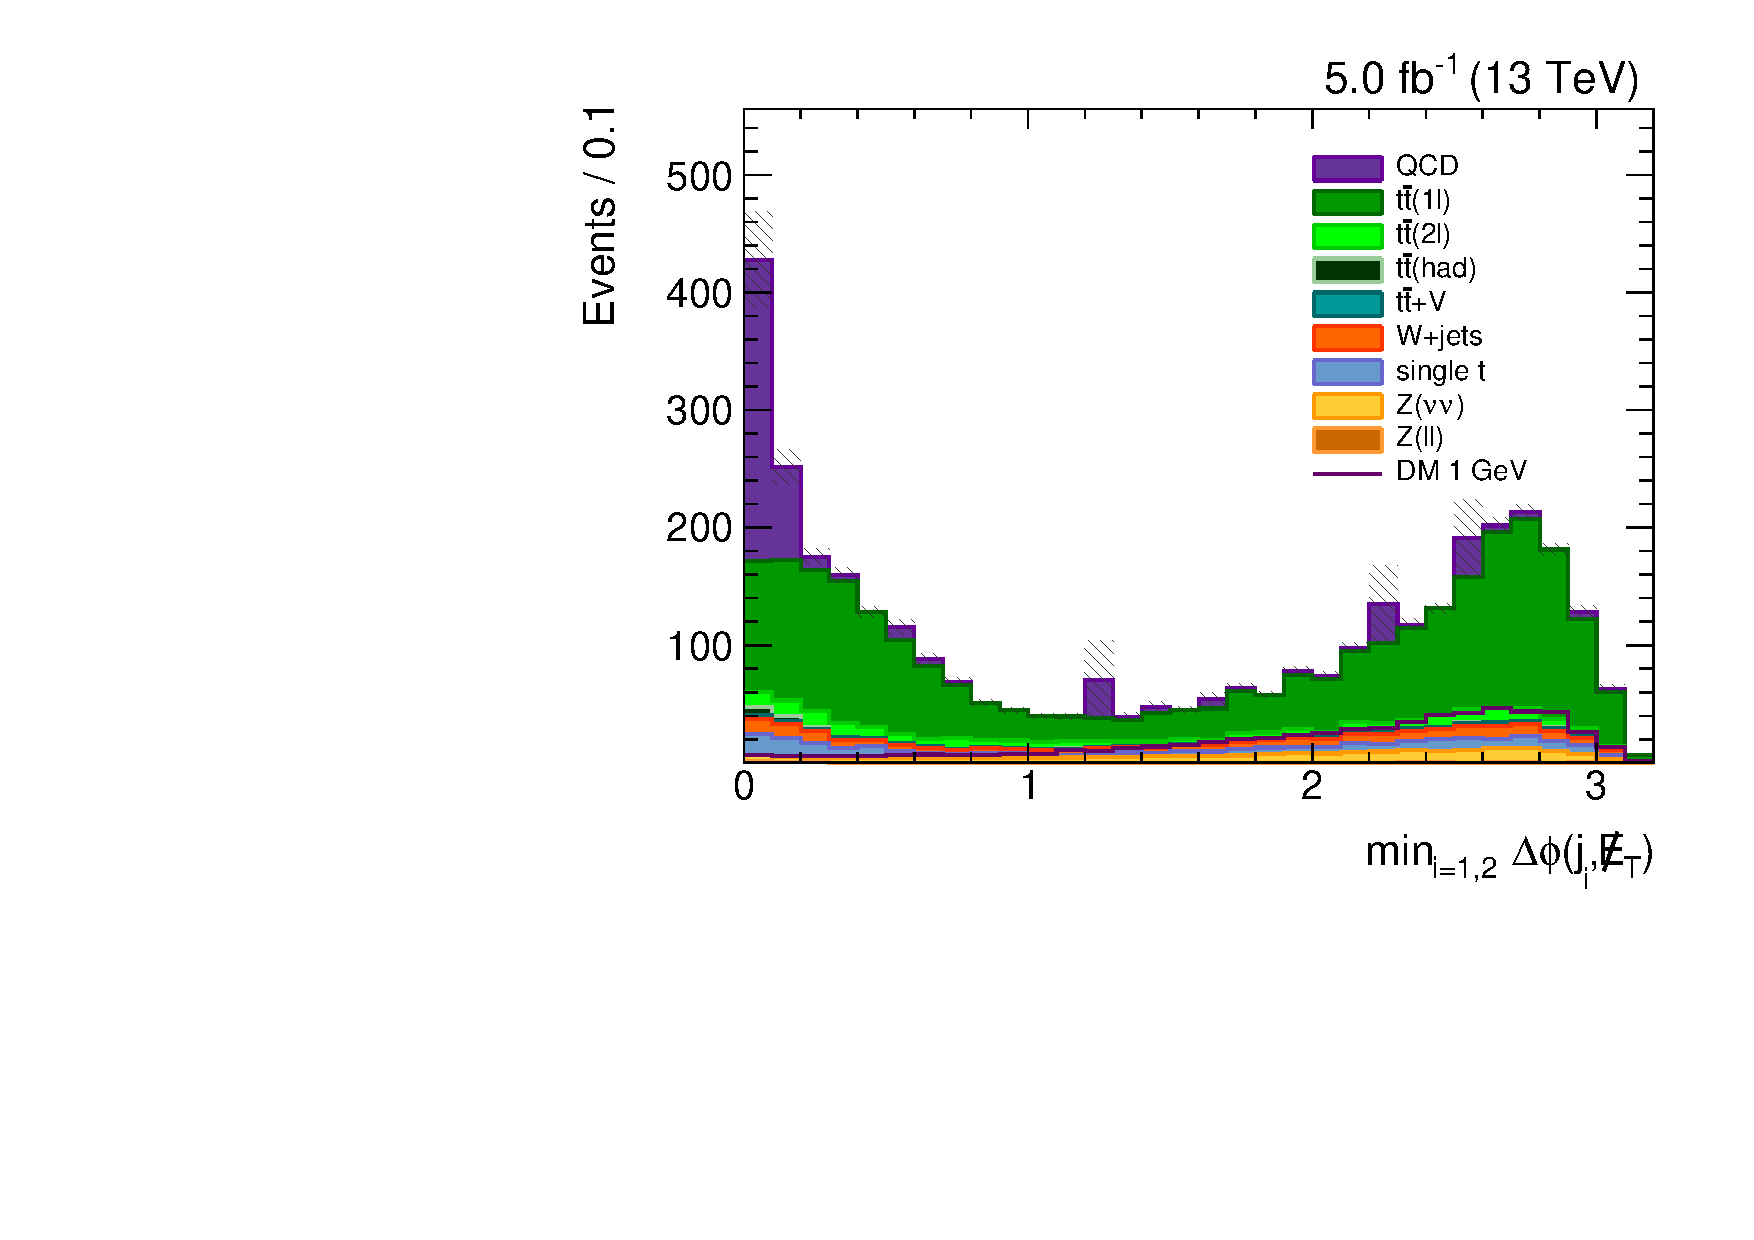
\includegraphics[width=0.32\textwidth]{figures/hadronic-incl-dphijetmet2.pdf}
  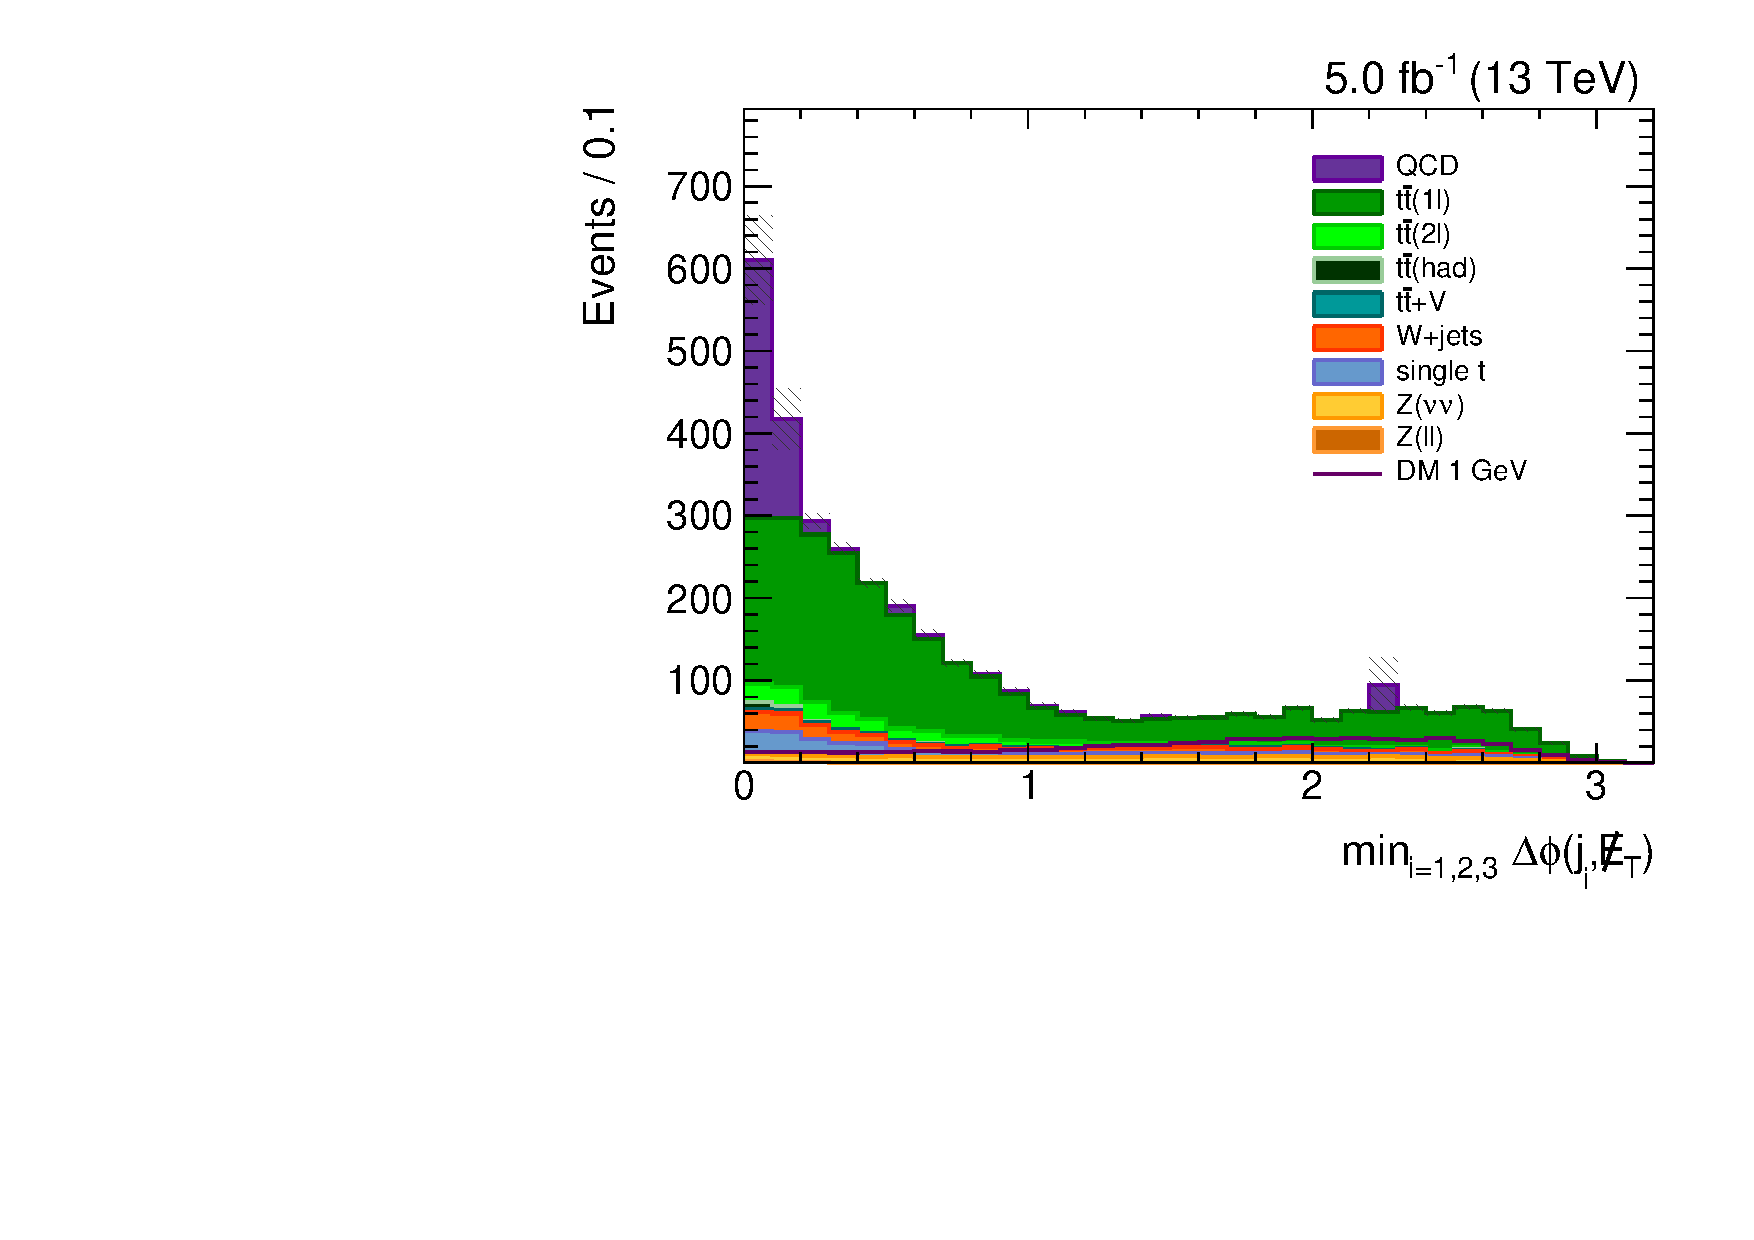
\includegraphics[width=0.32\textwidth]{figures/hadronic-incl-dphijetmet3.pdf}
  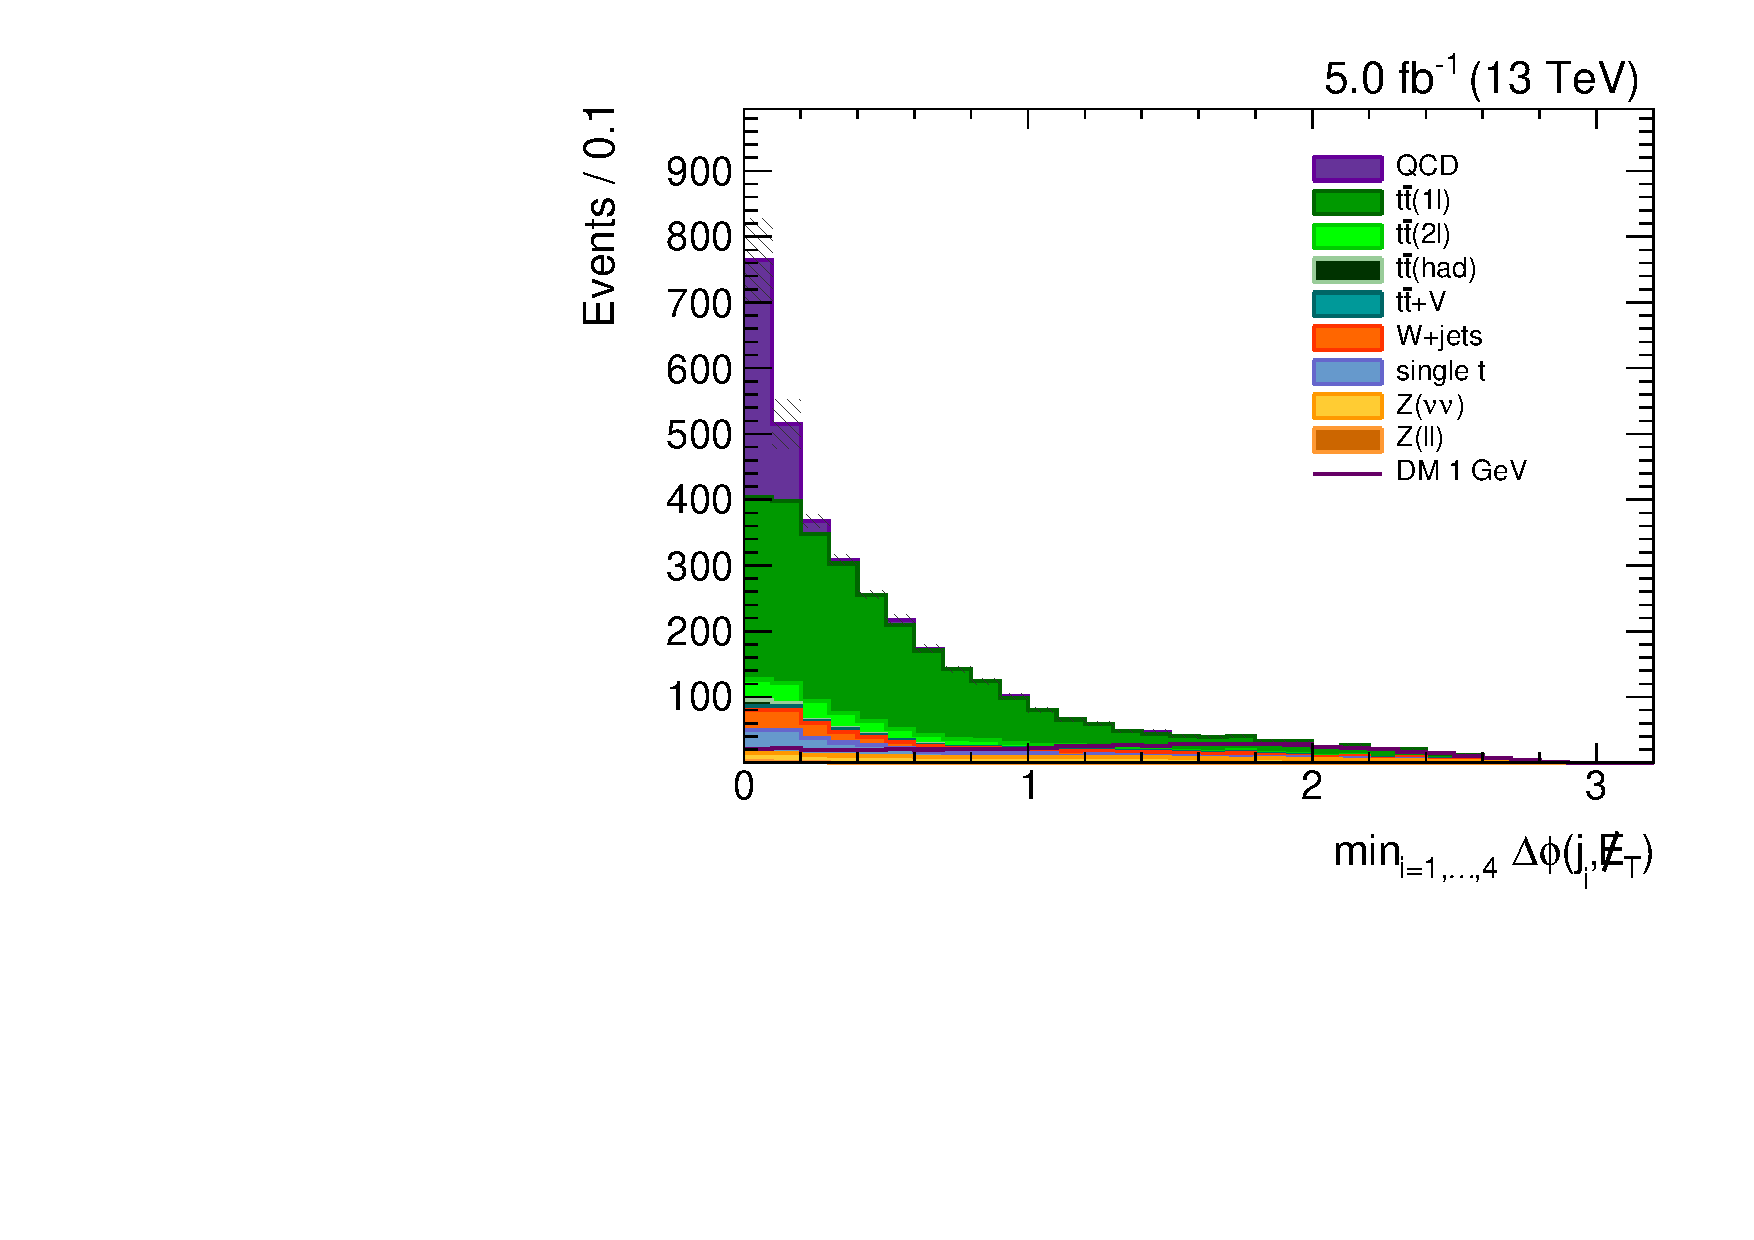
\includegraphics[width=0.32\textwidth]{figures/hadronic-incl-dphijetmet4.pdf} \\
  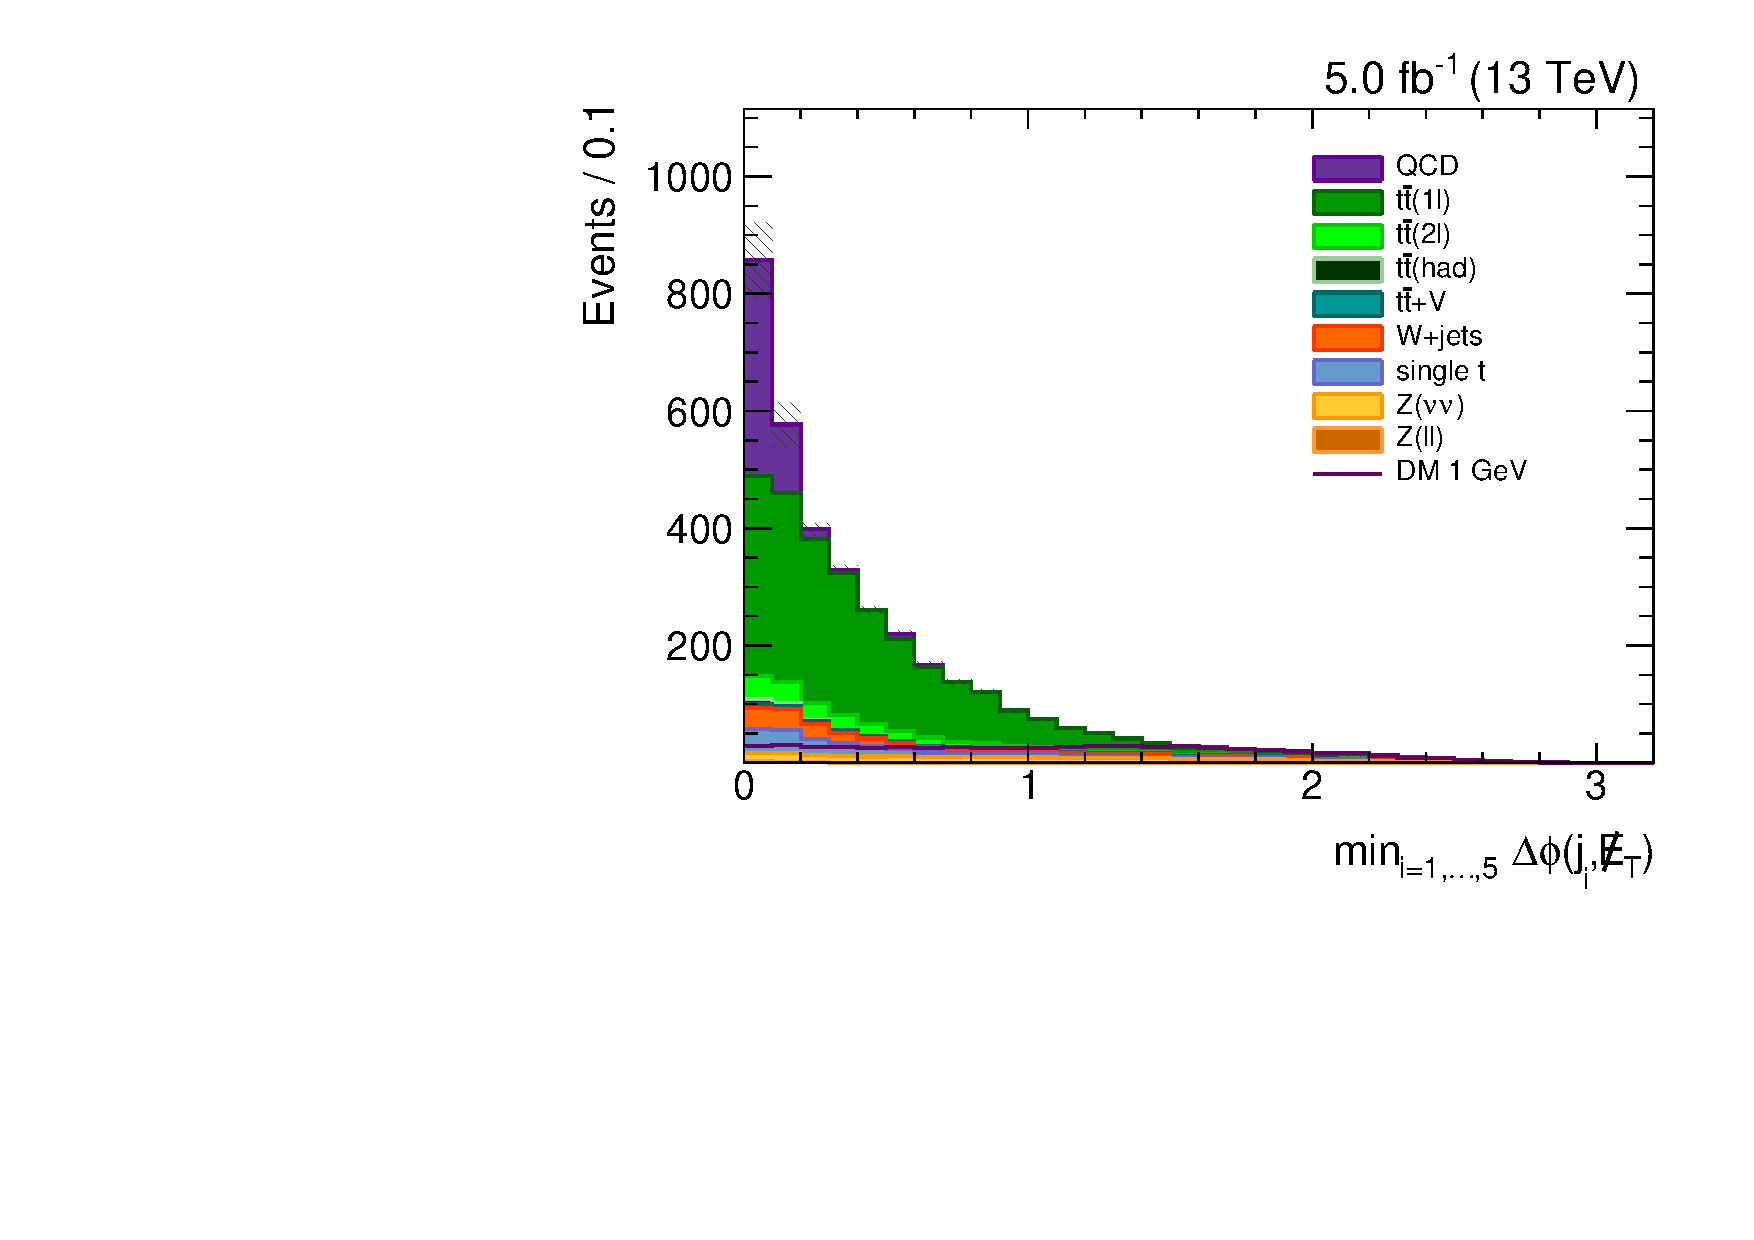
\includegraphics[width=0.32\textwidth]{figures/hadronic-incl-dphijetmet5.pdf}
  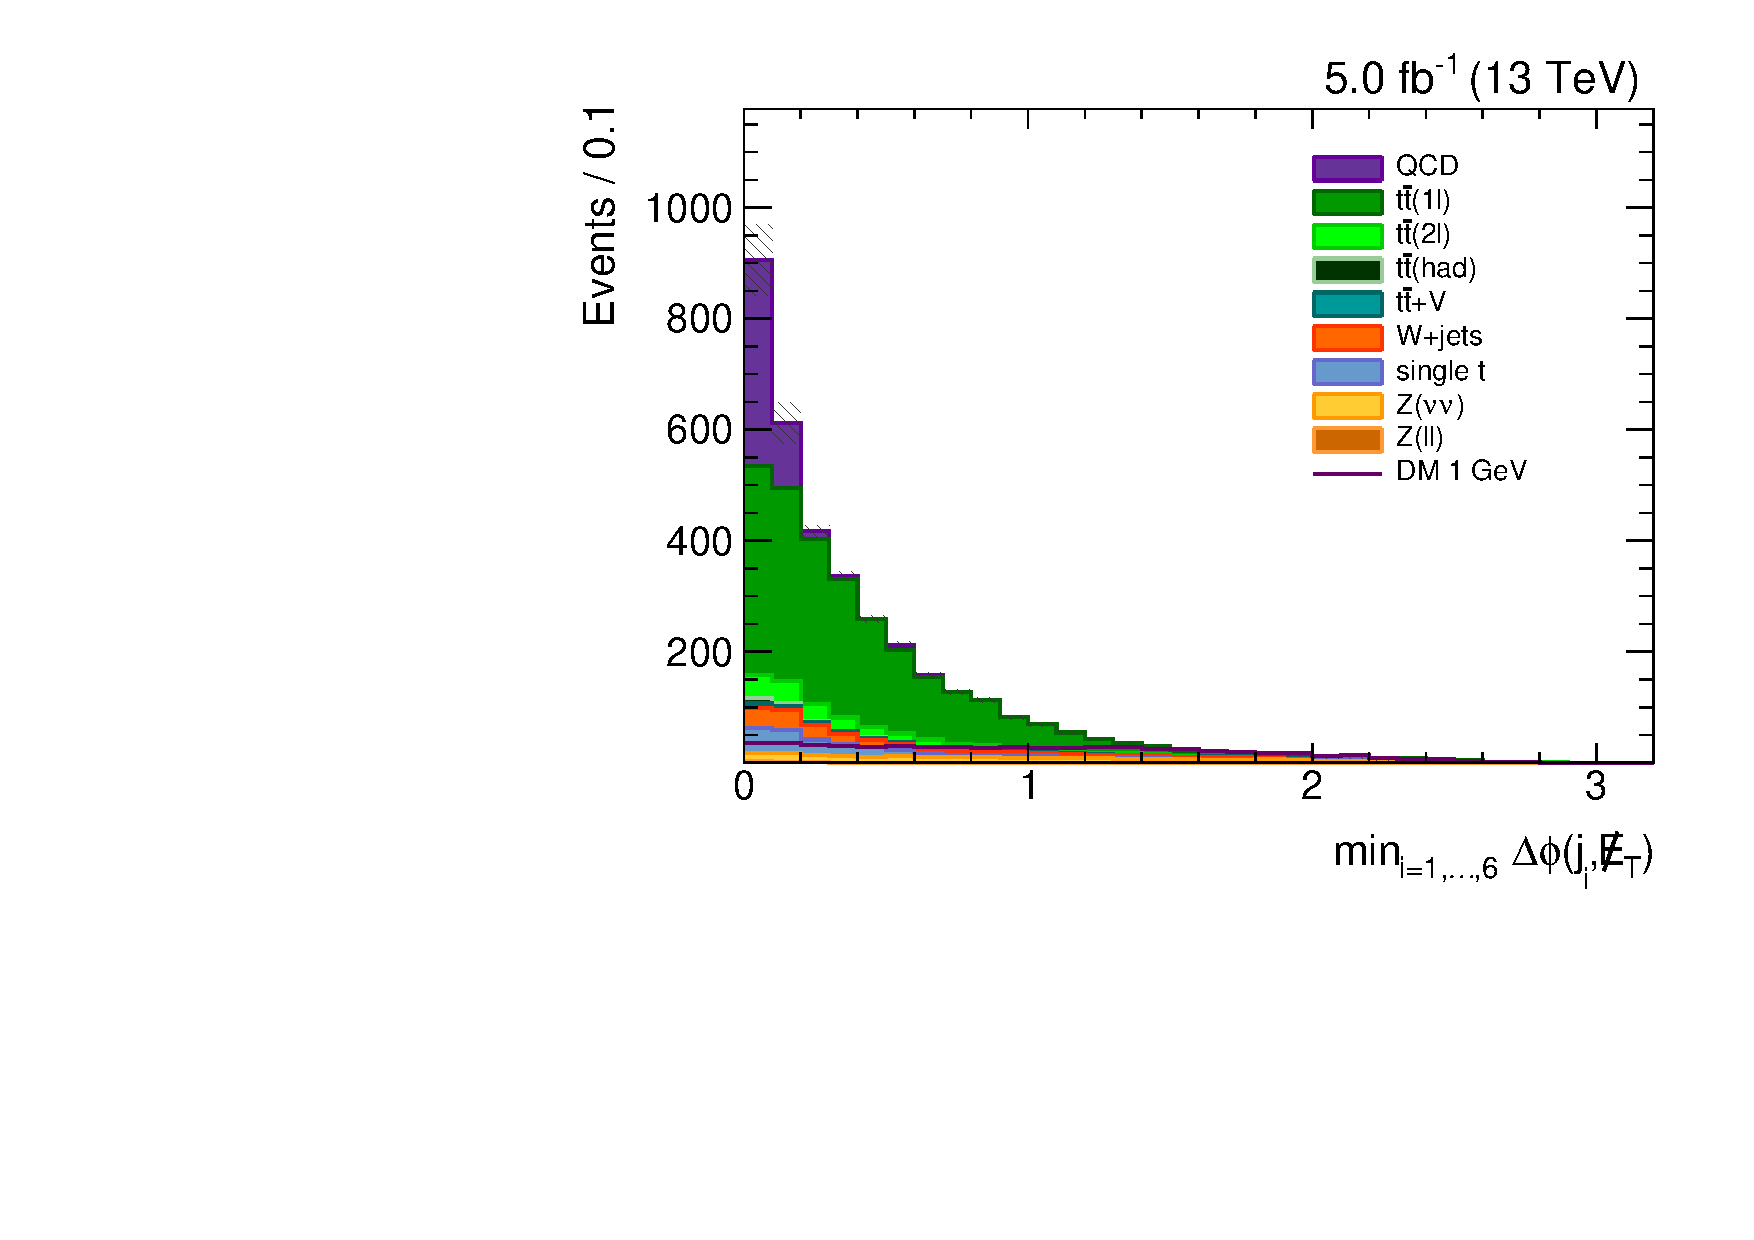
\includegraphics[width=0.32\textwidth]{figures/hadronic-incl-dphijetmet6.pdf}
  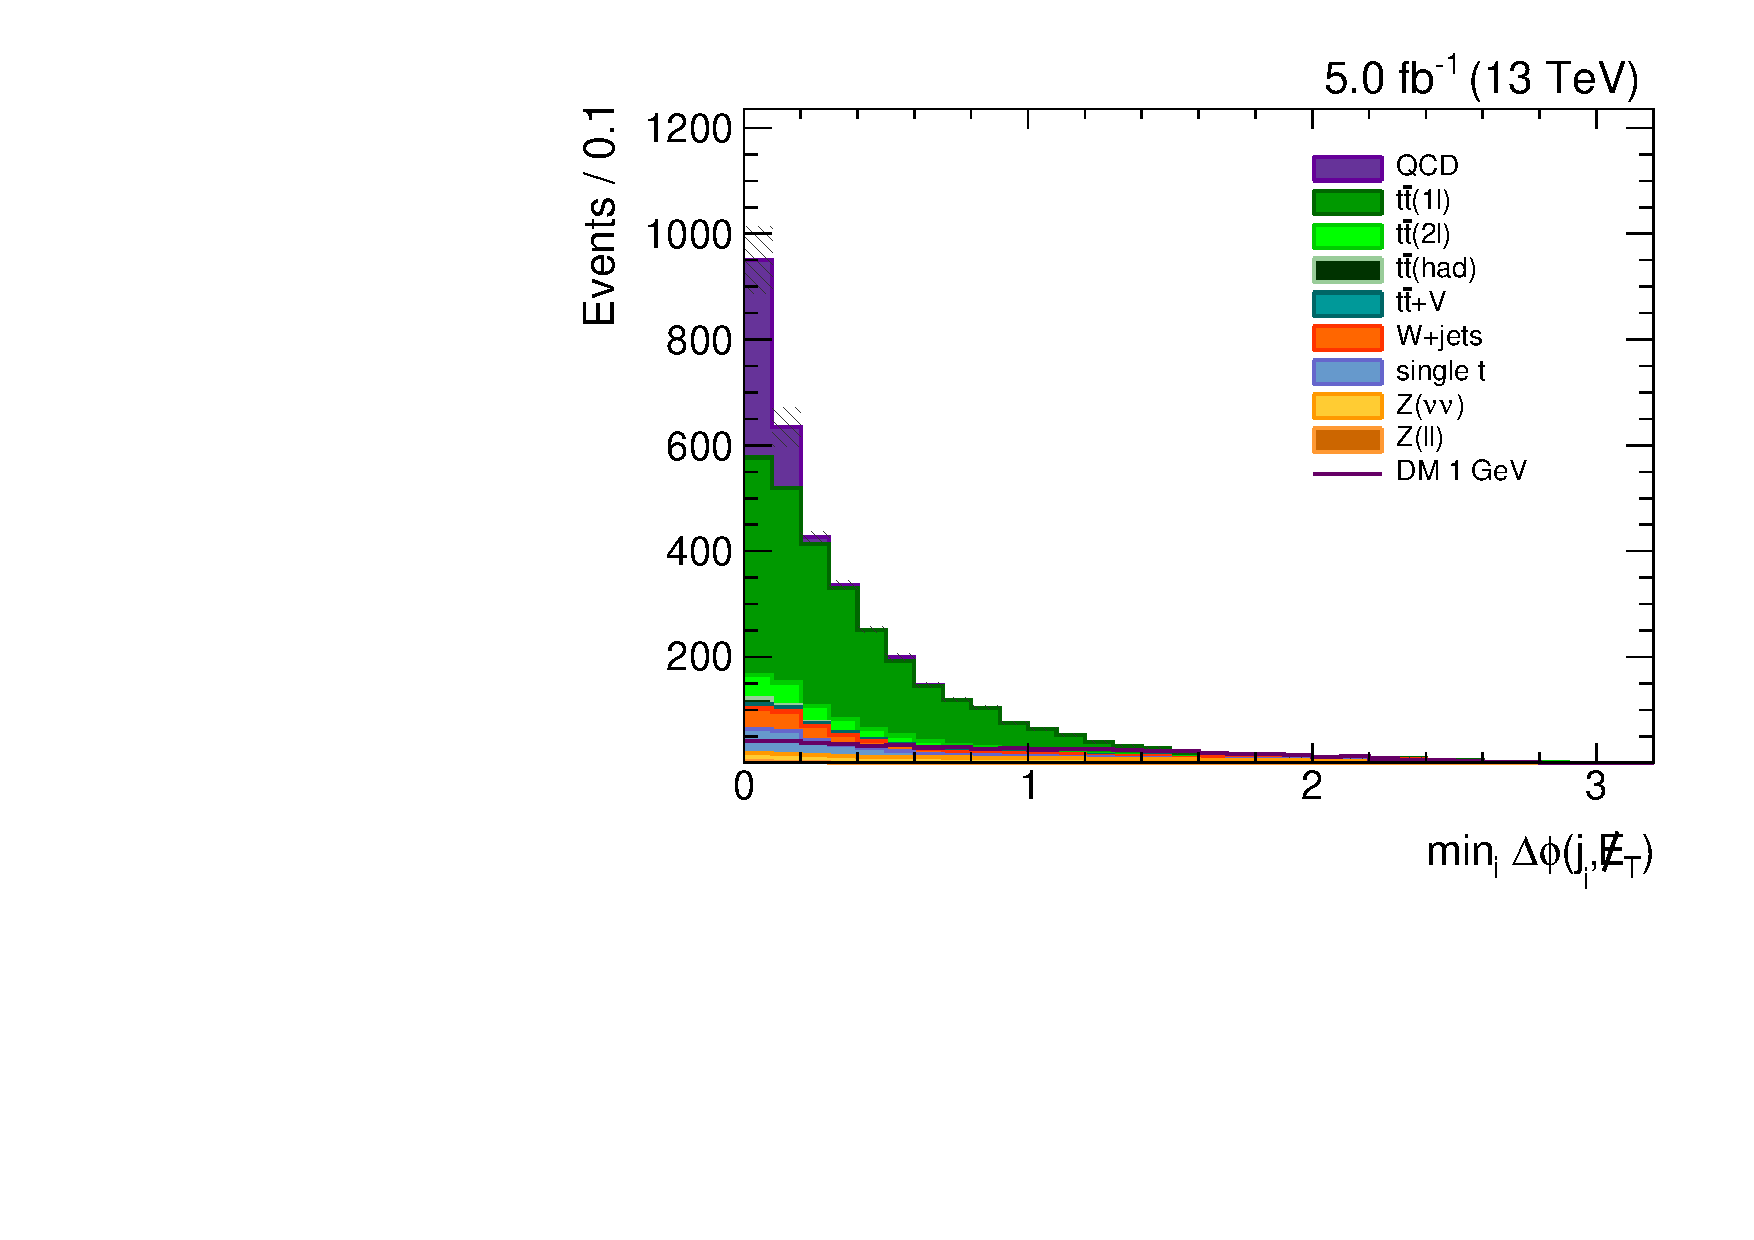
\includegraphics[width=0.32\textwidth]{figures/hadronic-incl-dphijetmet.pdf}
  \caption{$\Delta\phi$ distributions for various defintions.}
  \label{fig:hadronic_dphijetmet}
\end{figure}

\begin{figure}[htbp]
  \centering
  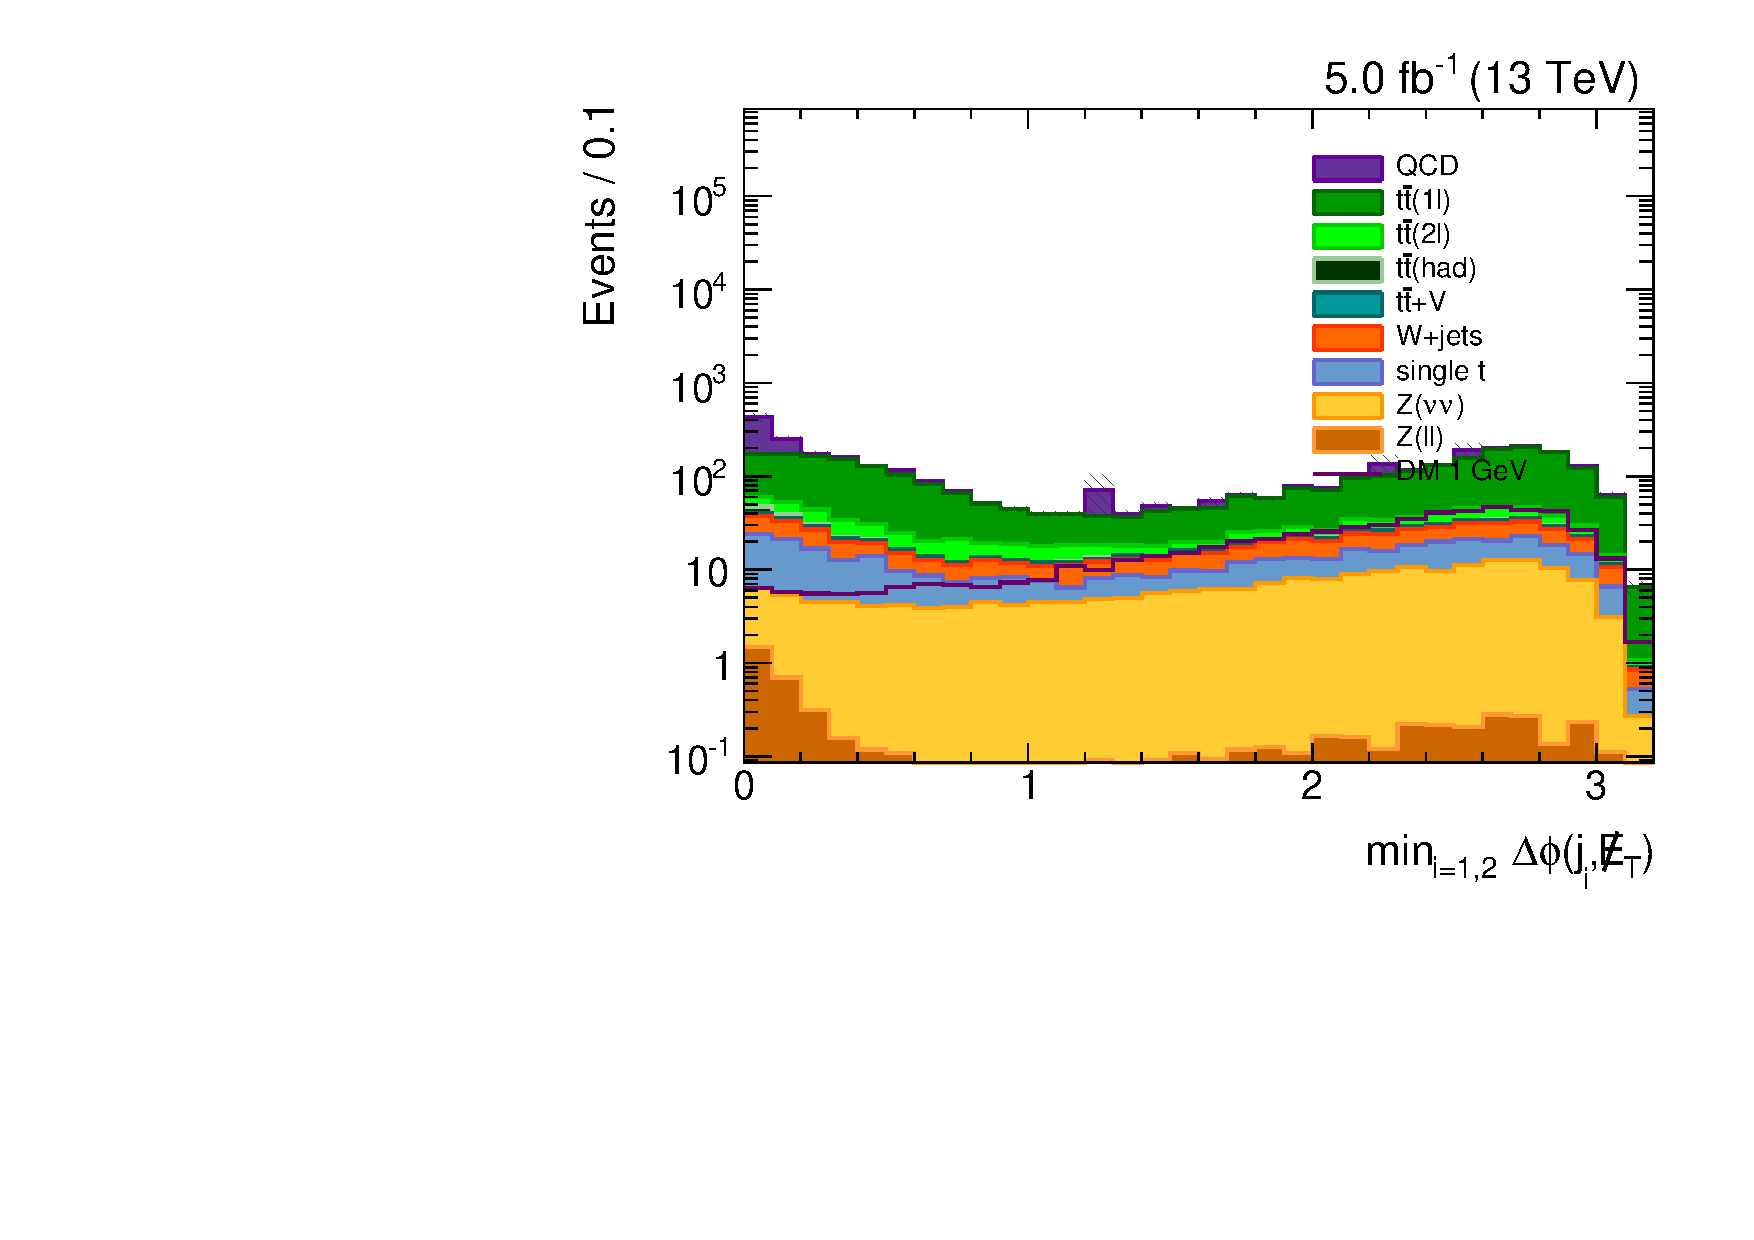
\includegraphics[width=0.32\textwidth]{figures/hadronic-incl-dphijetmet2log.pdf}
  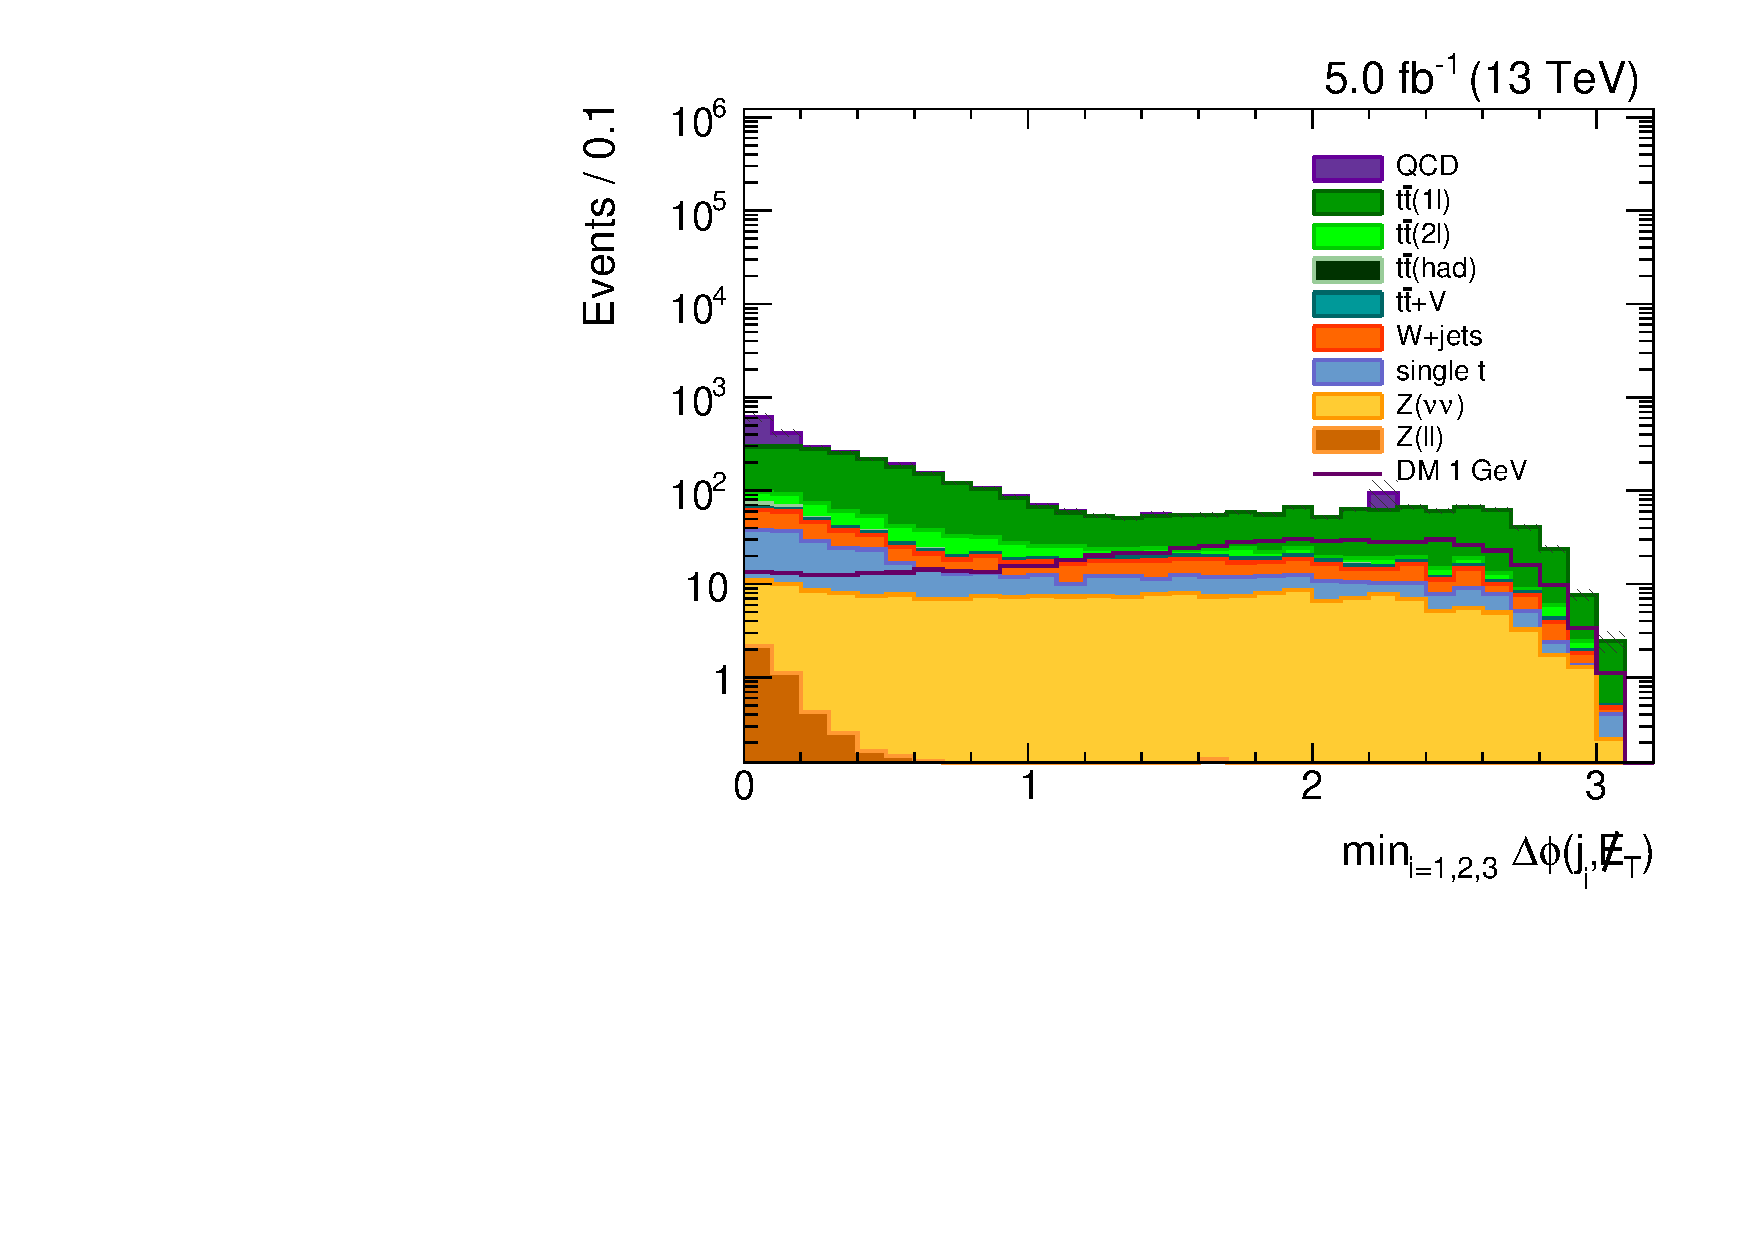
\includegraphics[width=0.32\textwidth]{figures/hadronic-incl-dphijetmet3log.pdf}
  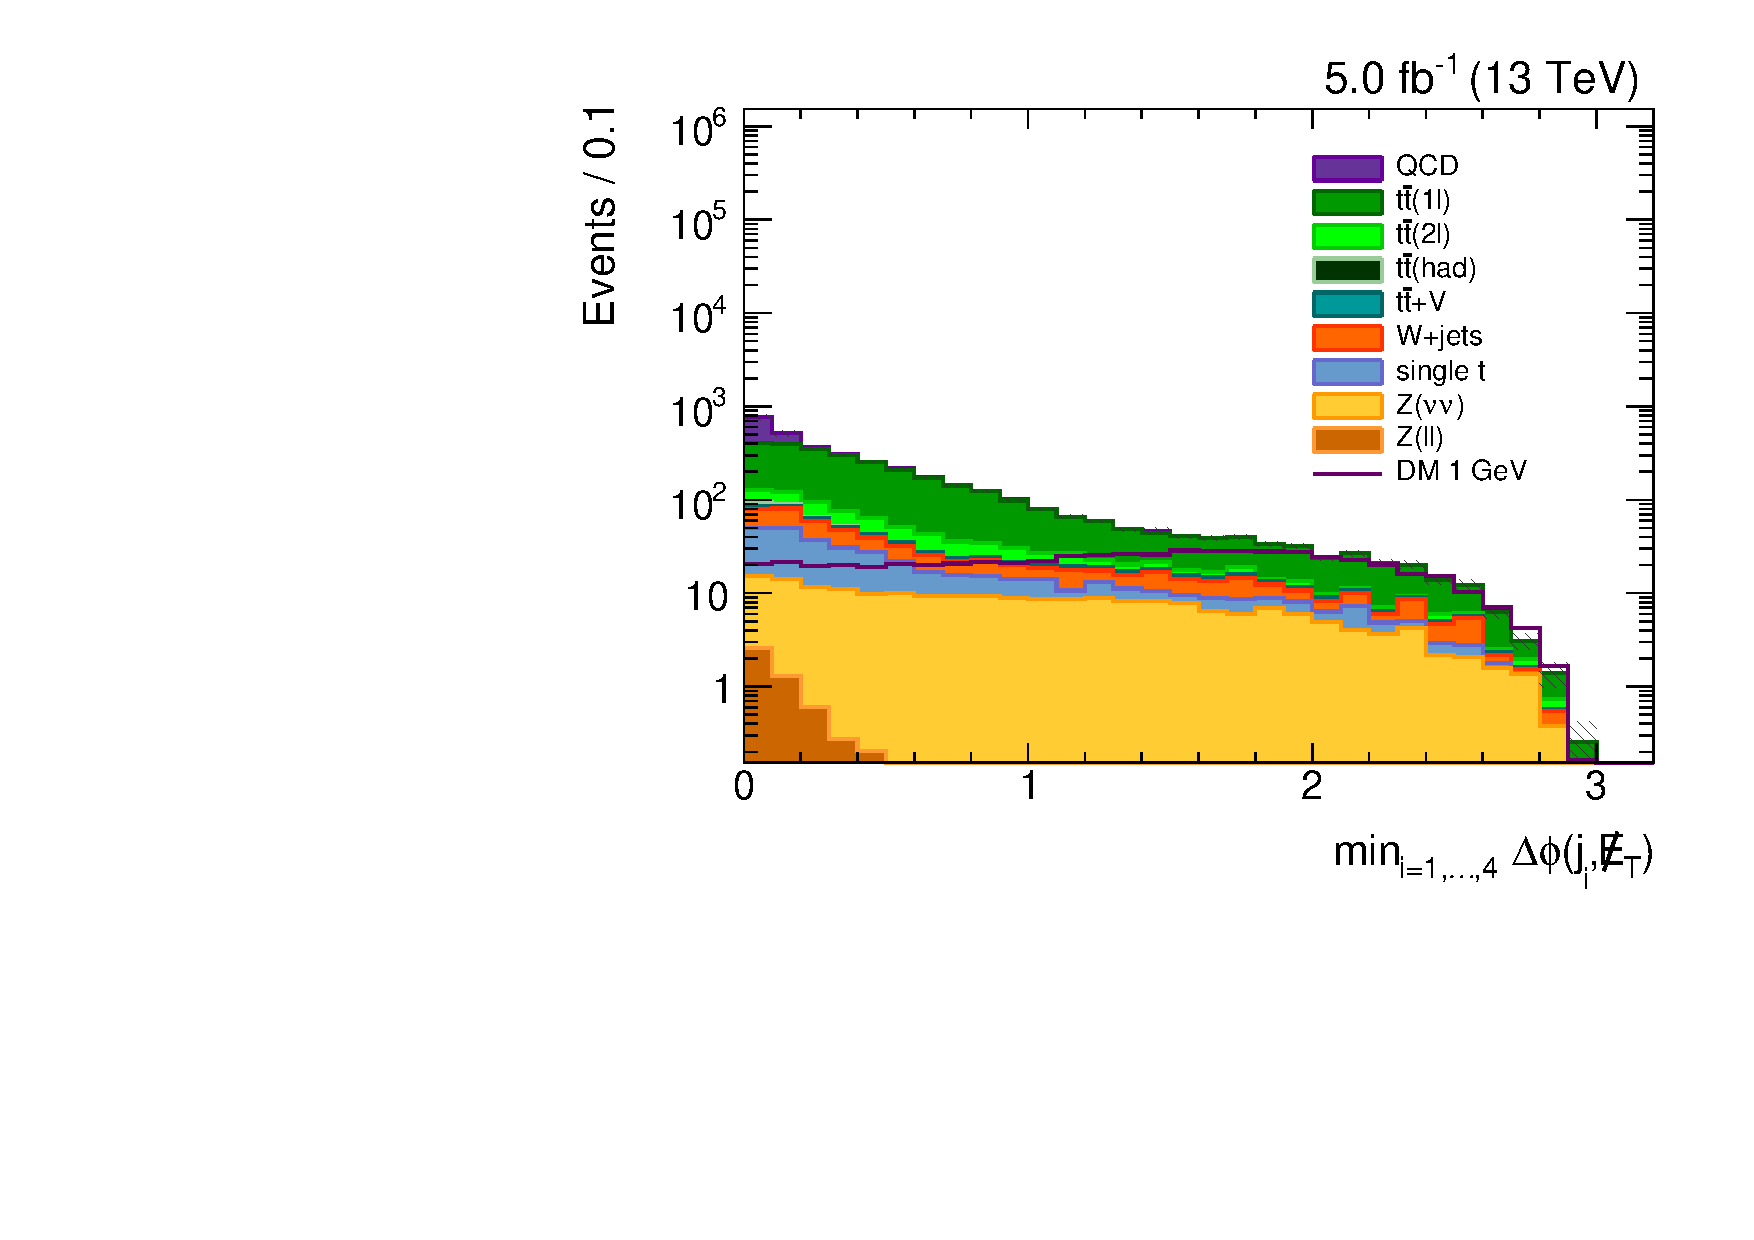
\includegraphics[width=0.32\textwidth]{figures/hadronic-incl-dphijetmet4log.pdf} \\
  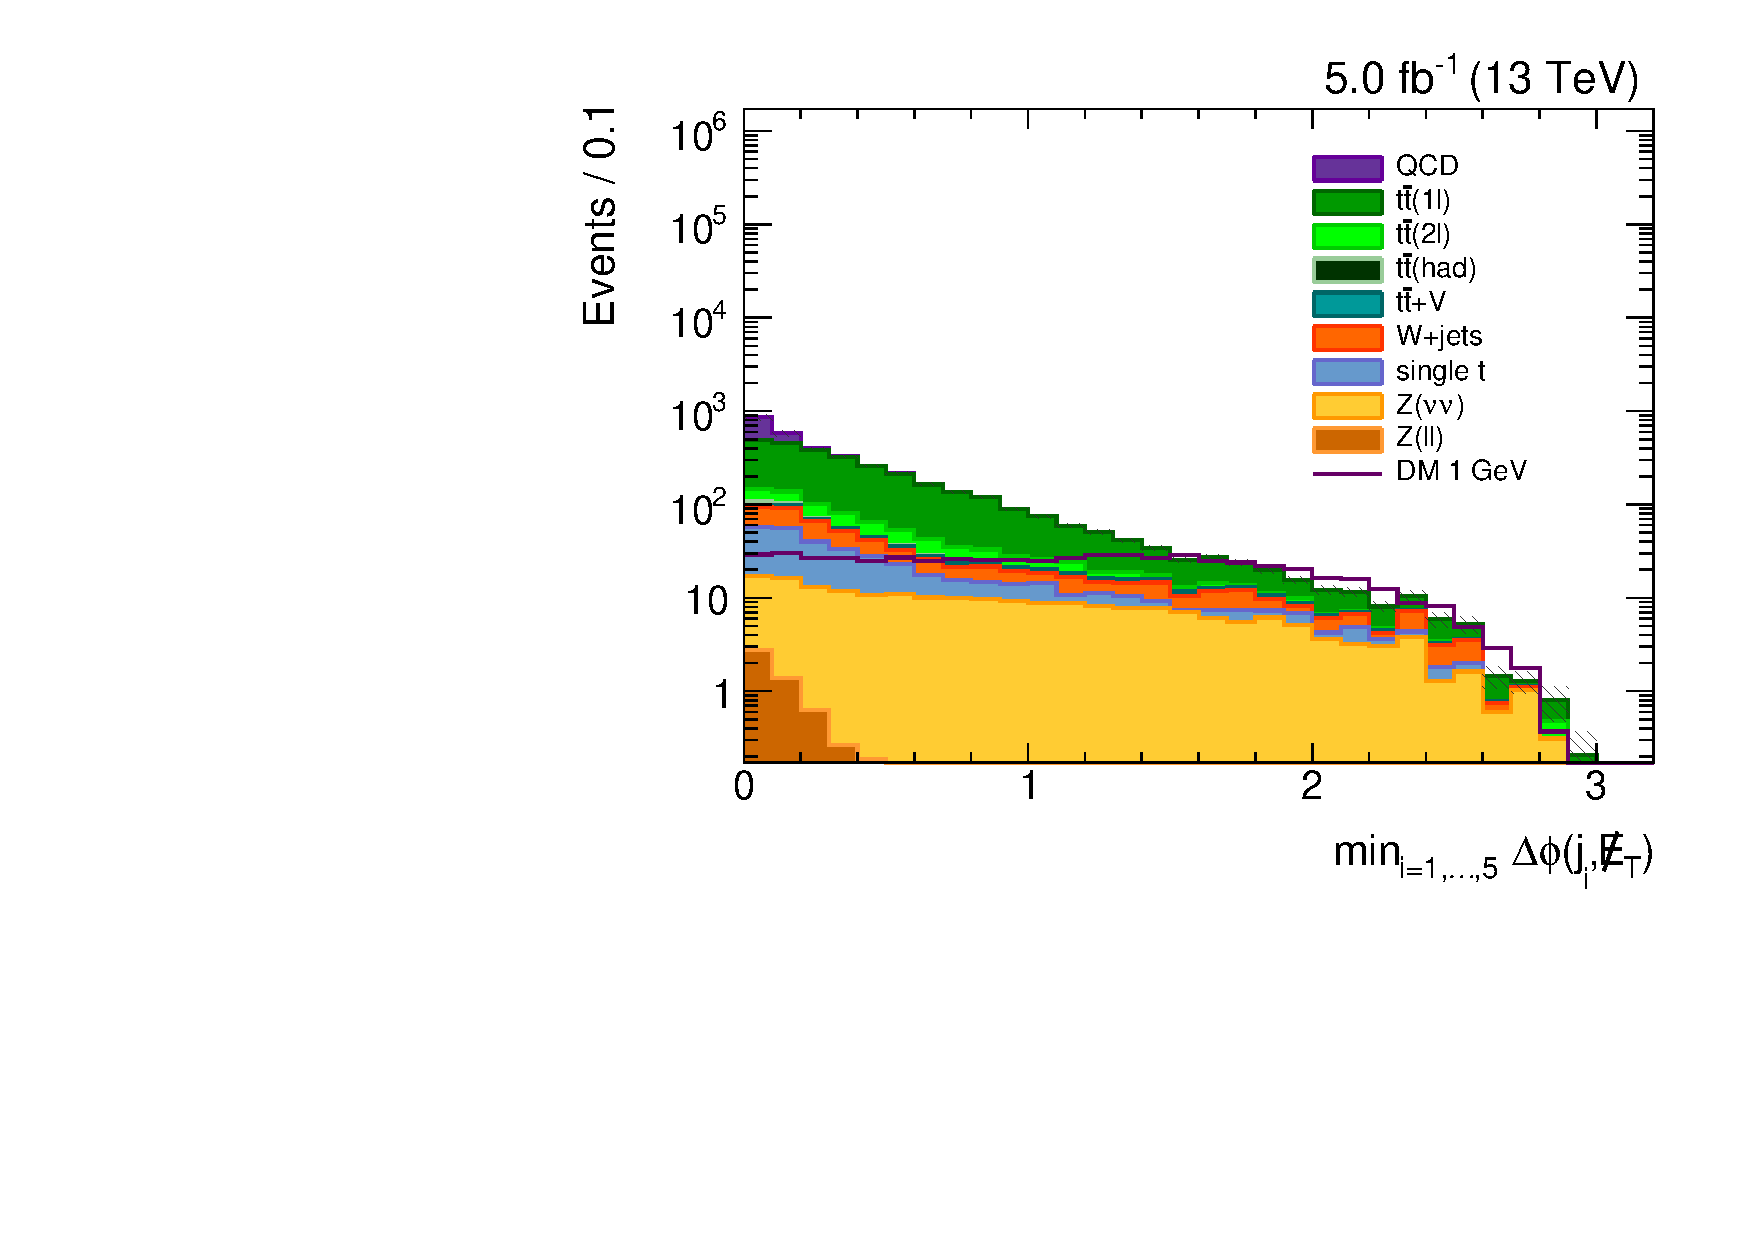
\includegraphics[width=0.32\textwidth]{figures/hadronic-incl-dphijetmet5log.pdf}
  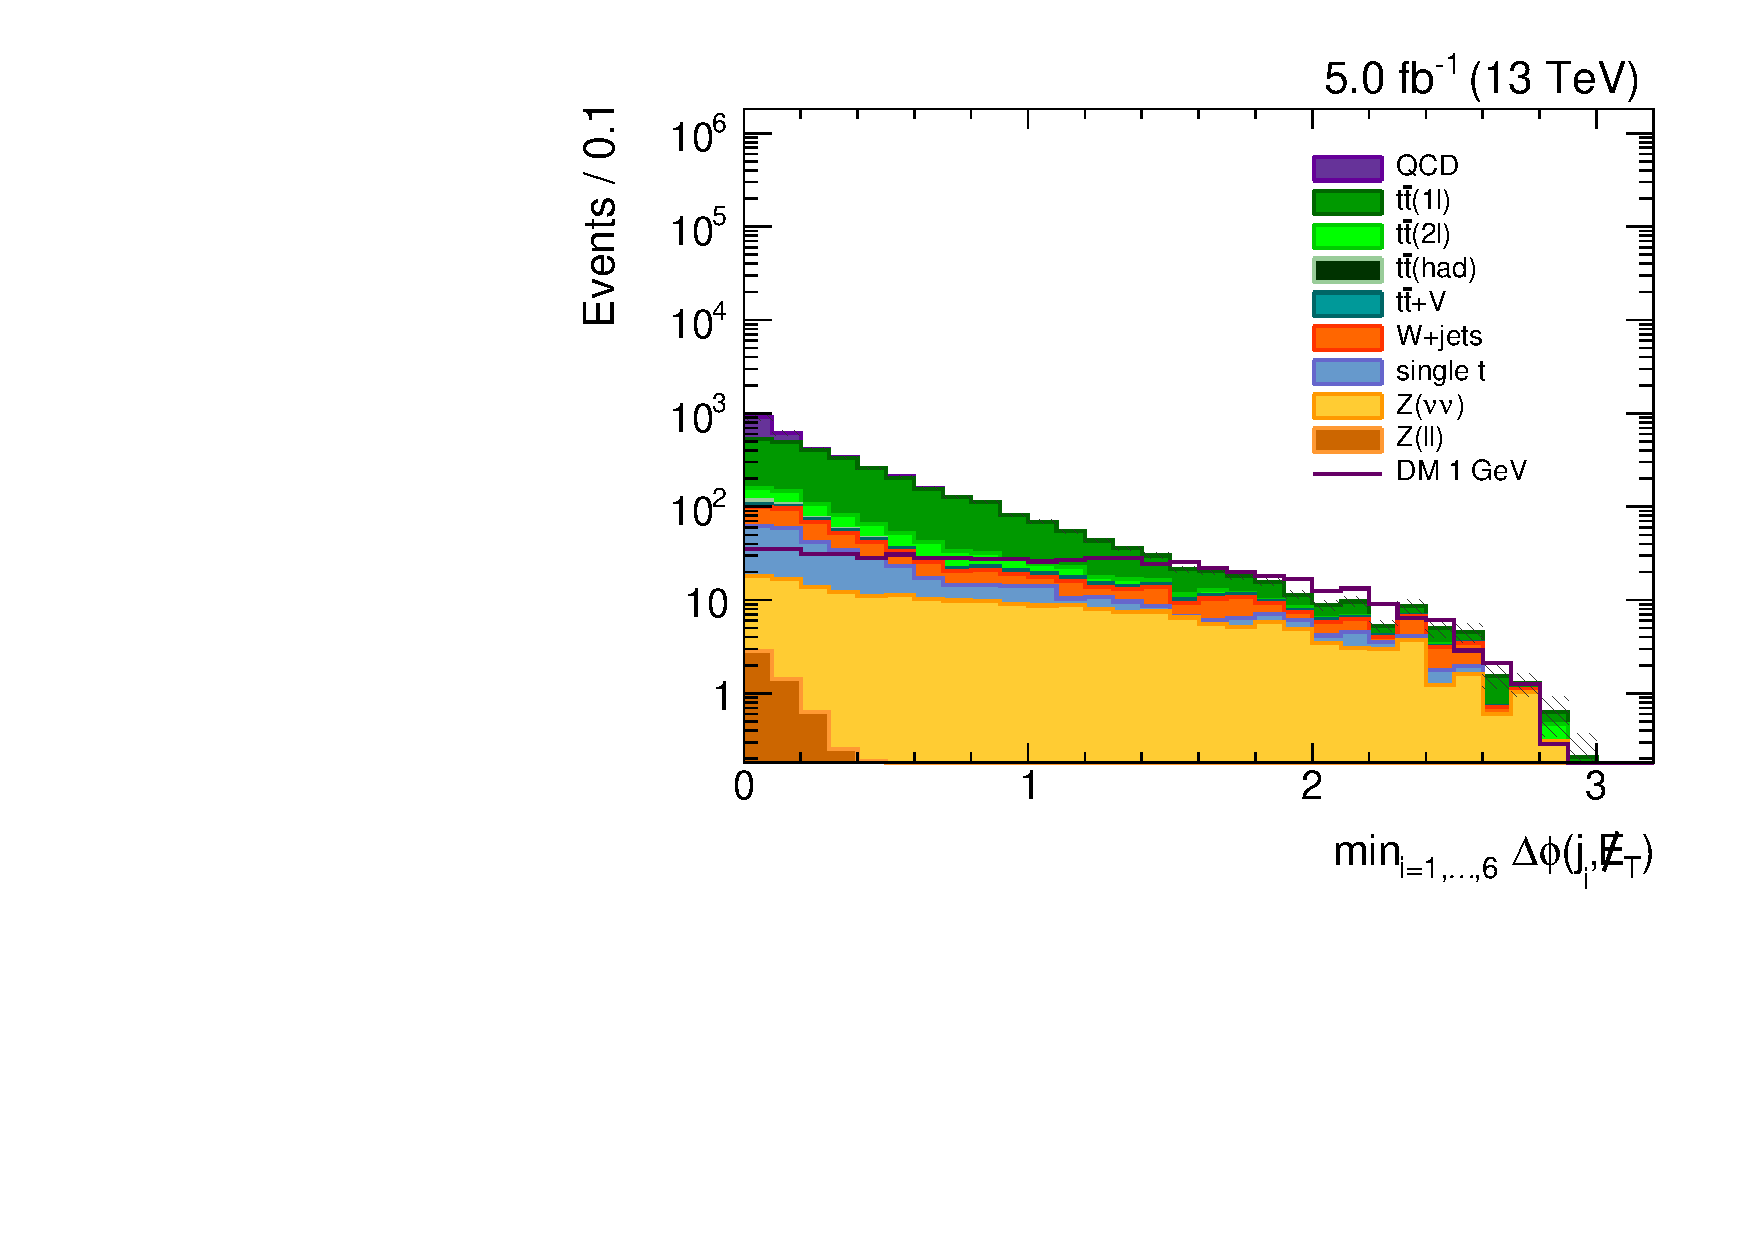
\includegraphics[width=0.32\textwidth]{figures/hadronic-incl-dphijetmet6log.pdf}
  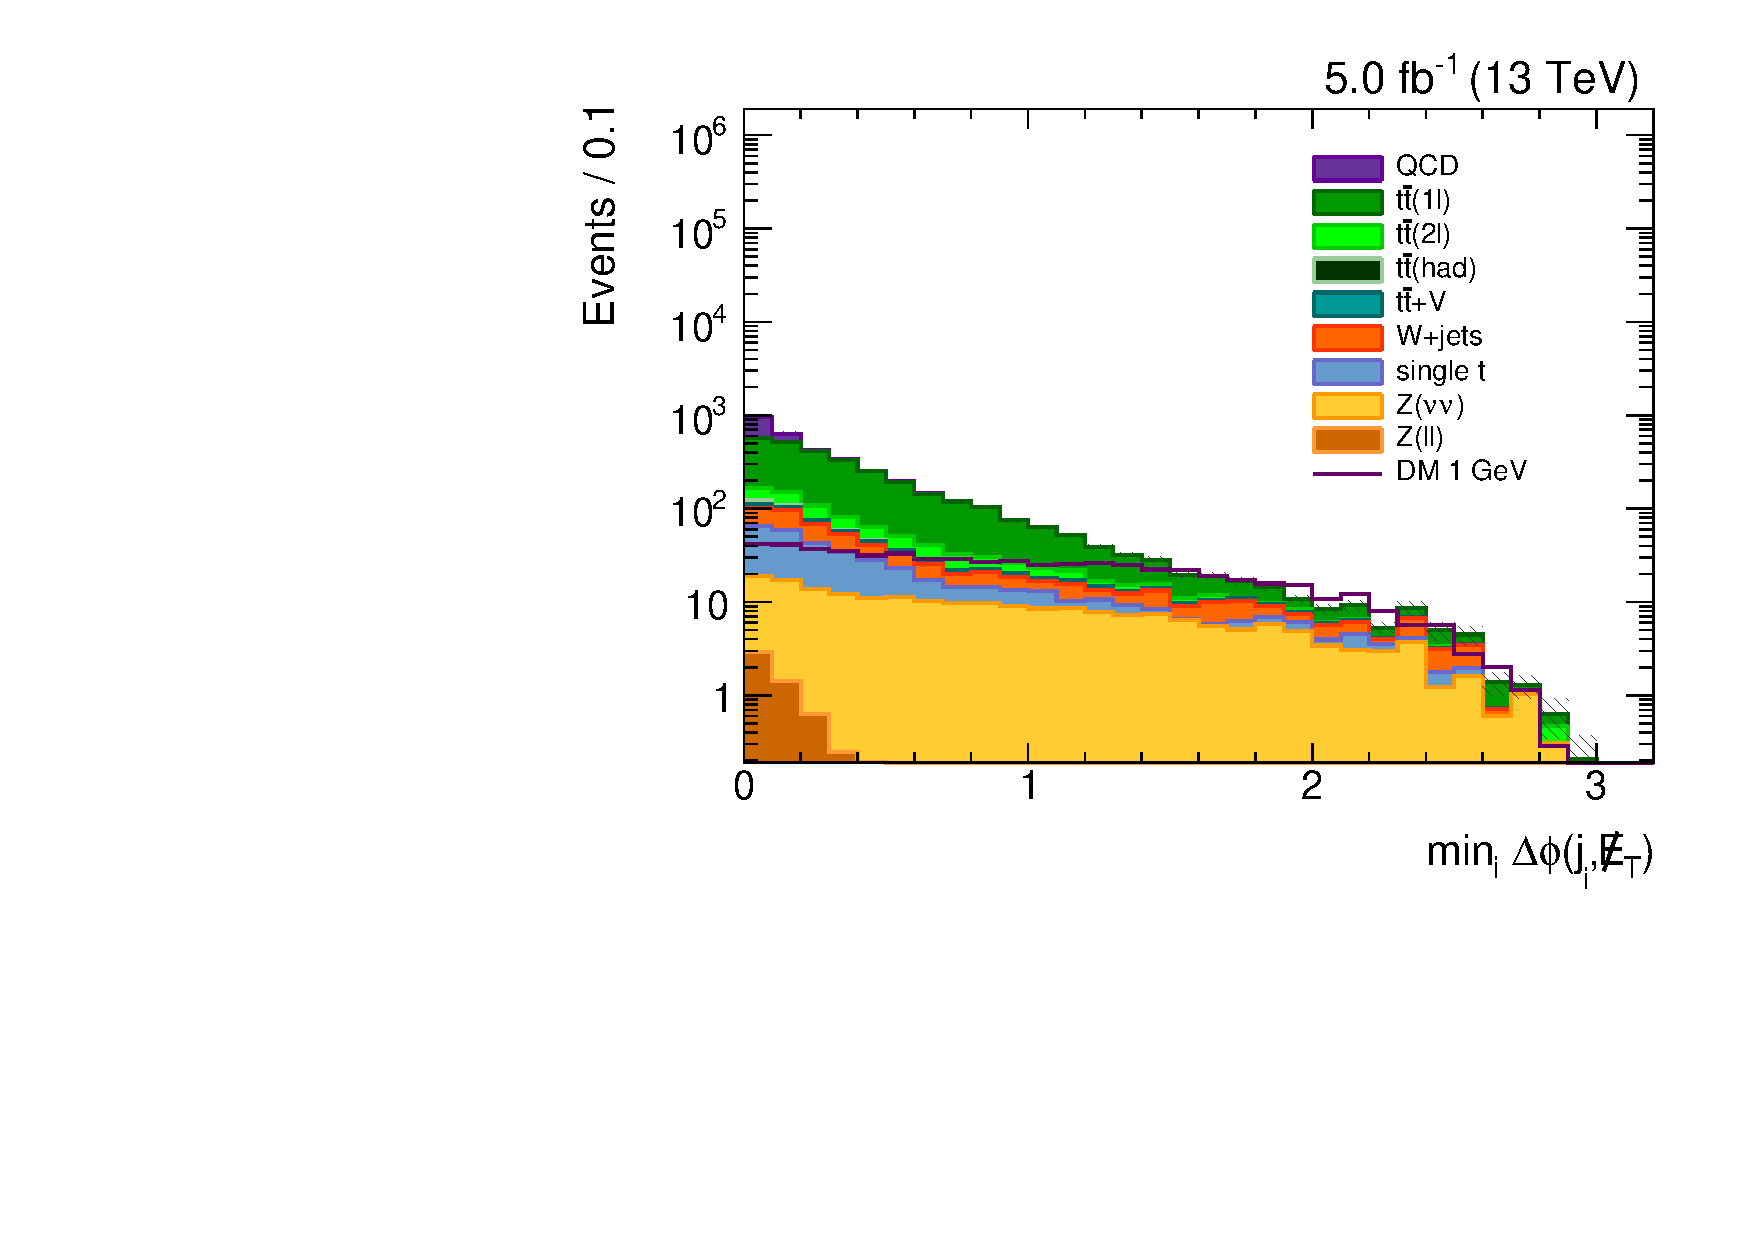
\includegraphics[width=0.32\textwidth]{figures/hadronic-incl-dphijetmetlog.pdf}
  \caption{$\Delta\phi$ distributions for various definitions in log scale.}
  \label{fig:hadronic_dphijetmetlog}
\end{figure}

\begin{figure}[htbp]
  \centering
  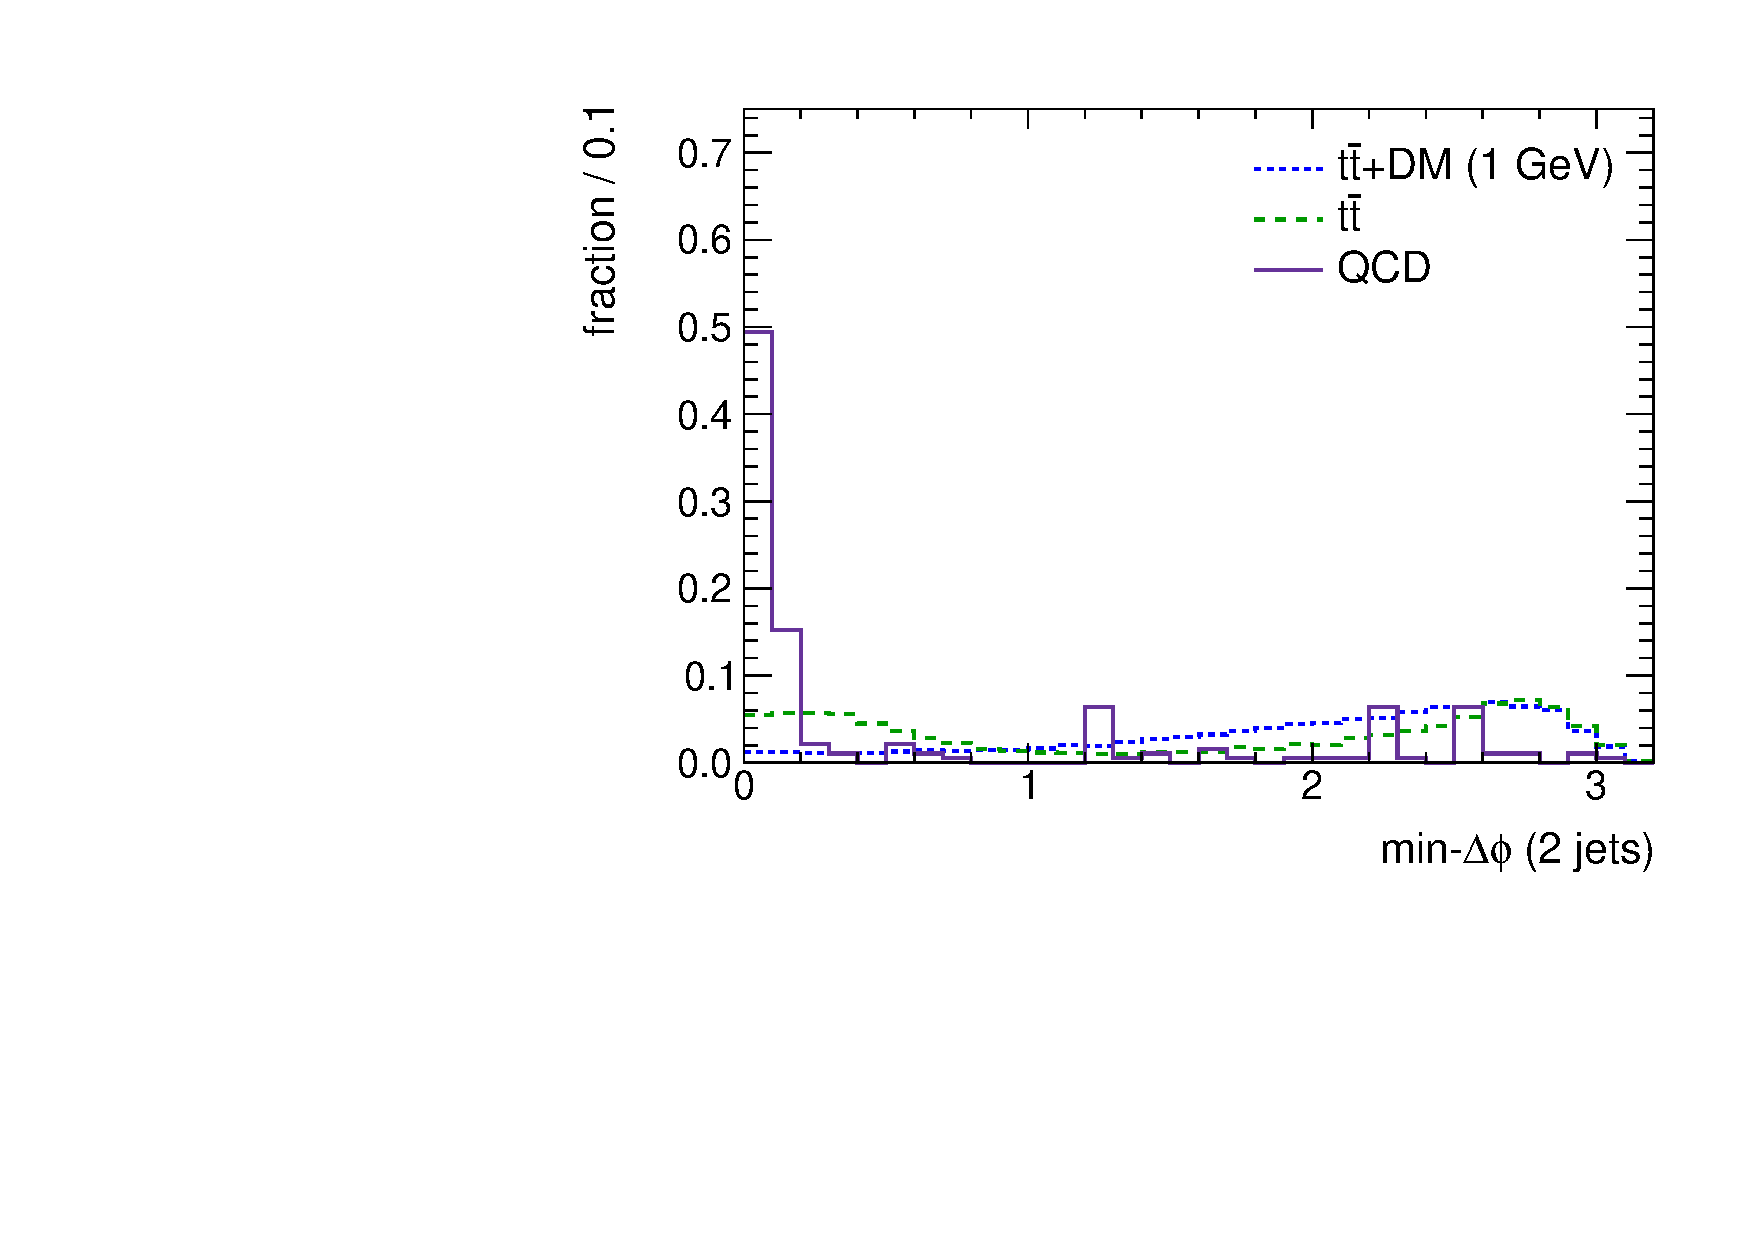
\includegraphics[width=0.32\textwidth]{figures/hadronic-overlay-dphijetmet2.pdf}
  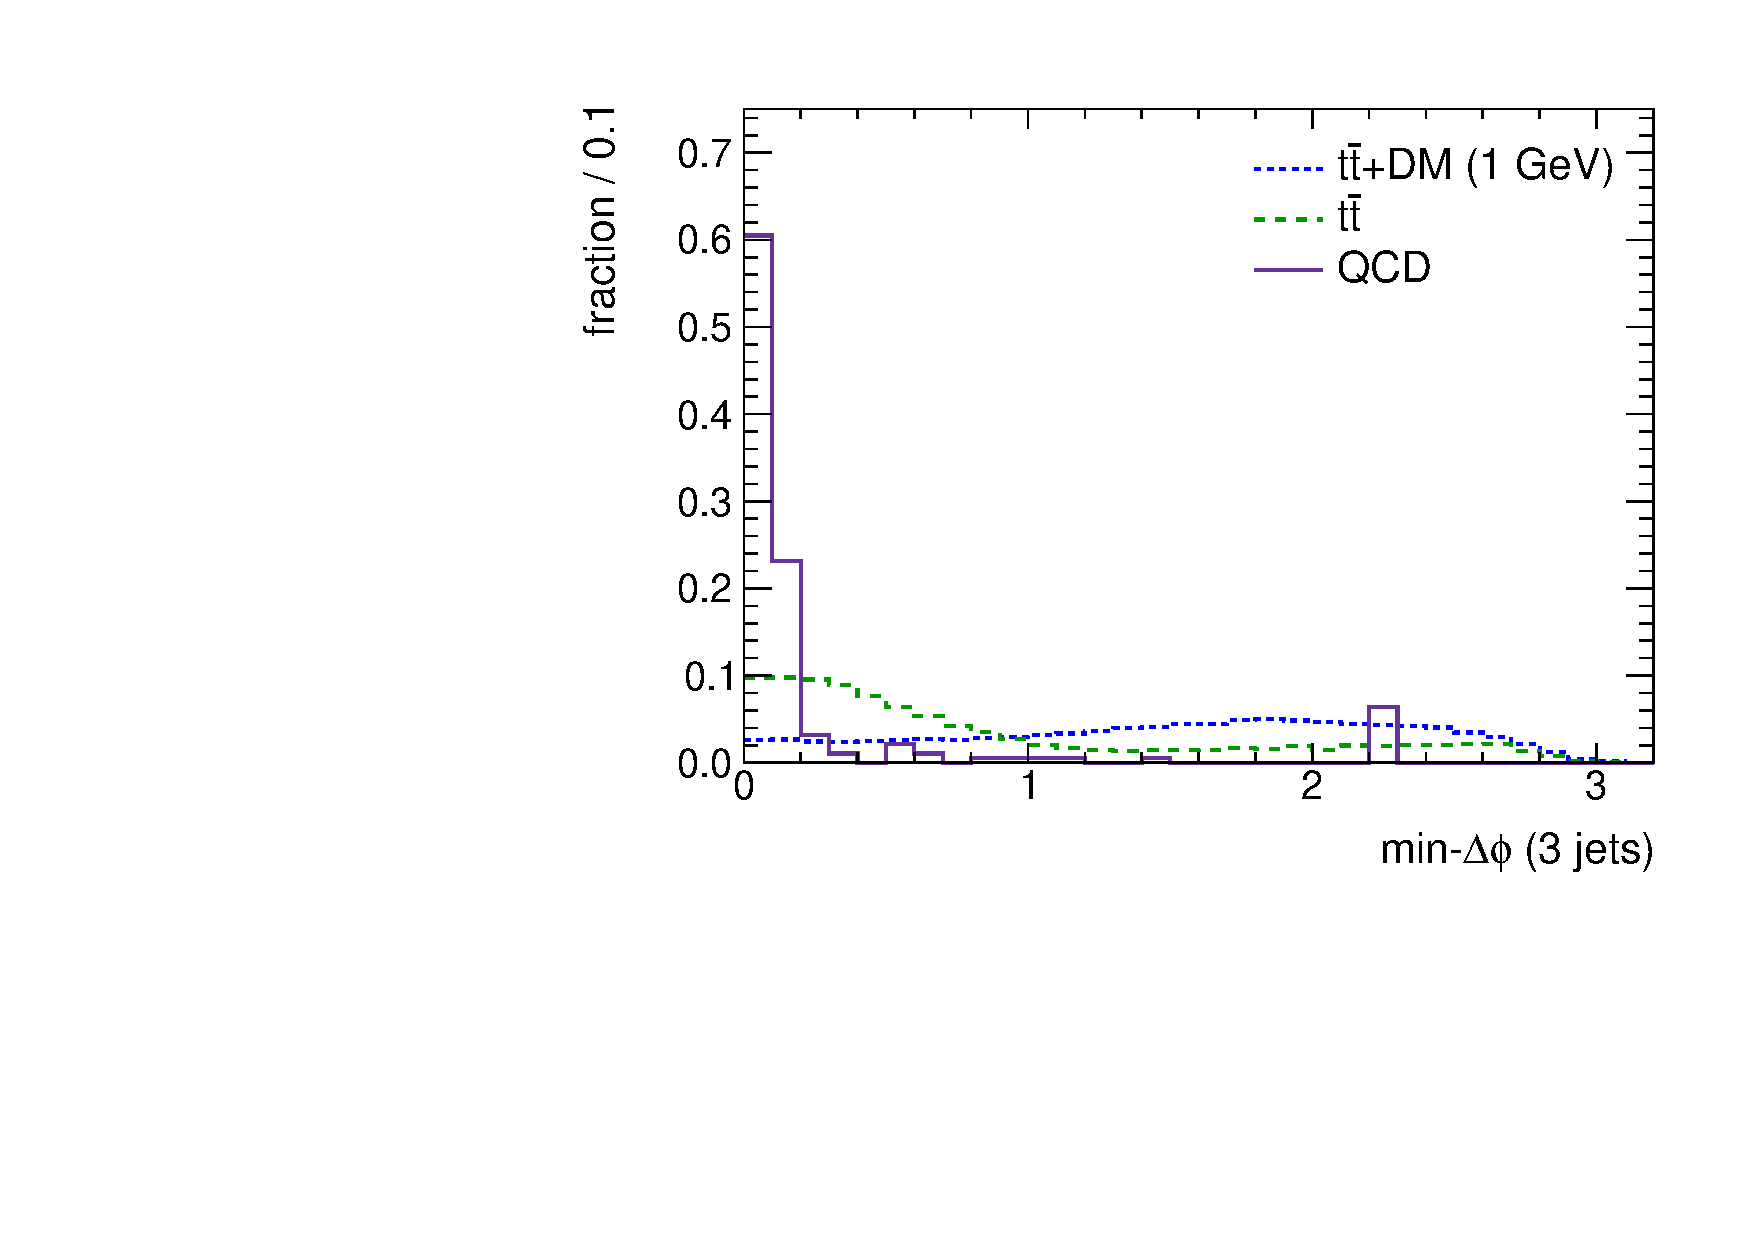
\includegraphics[width=0.32\textwidth]{figures/hadronic-overlay-dphijetmet3.pdf}
  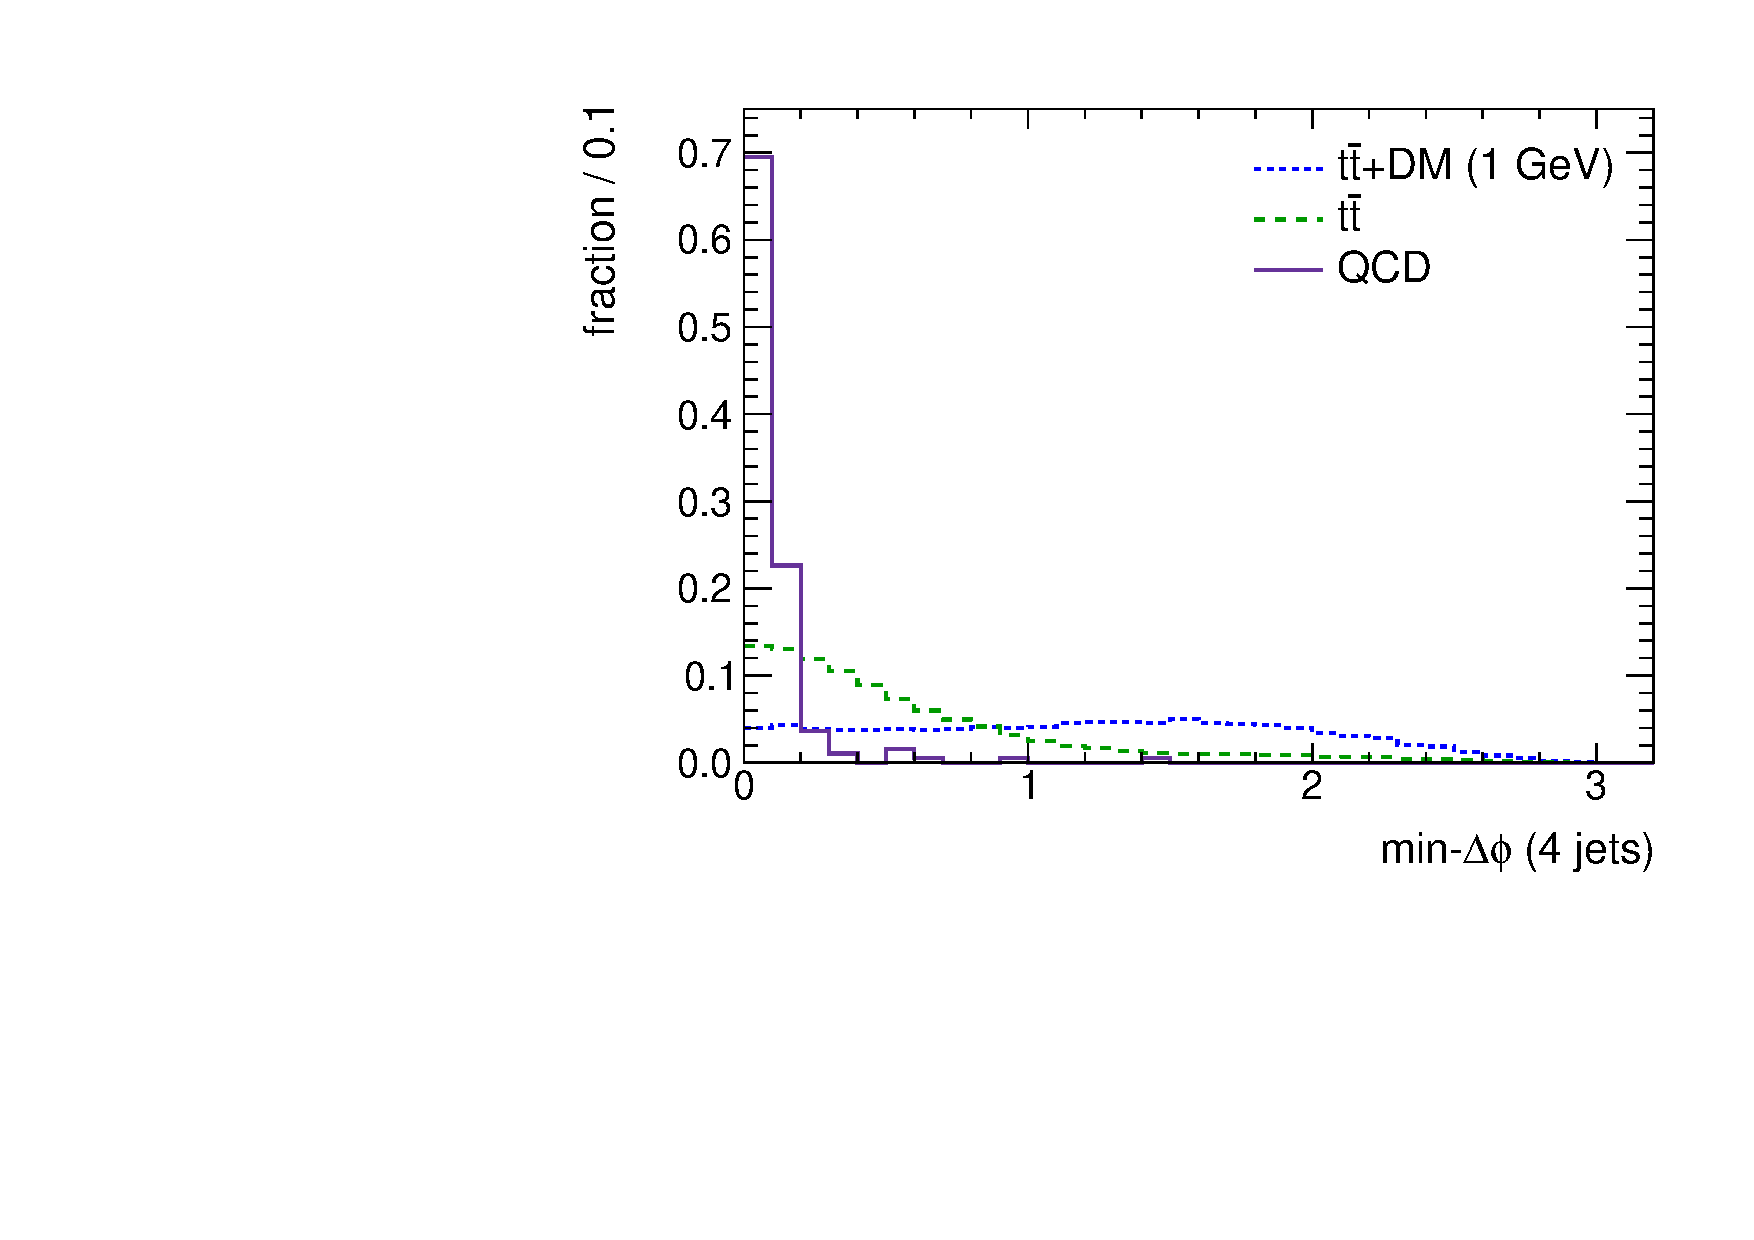
\includegraphics[width=0.32\textwidth]{figures/hadronic-overlay-dphijetmet4.pdf} \\
  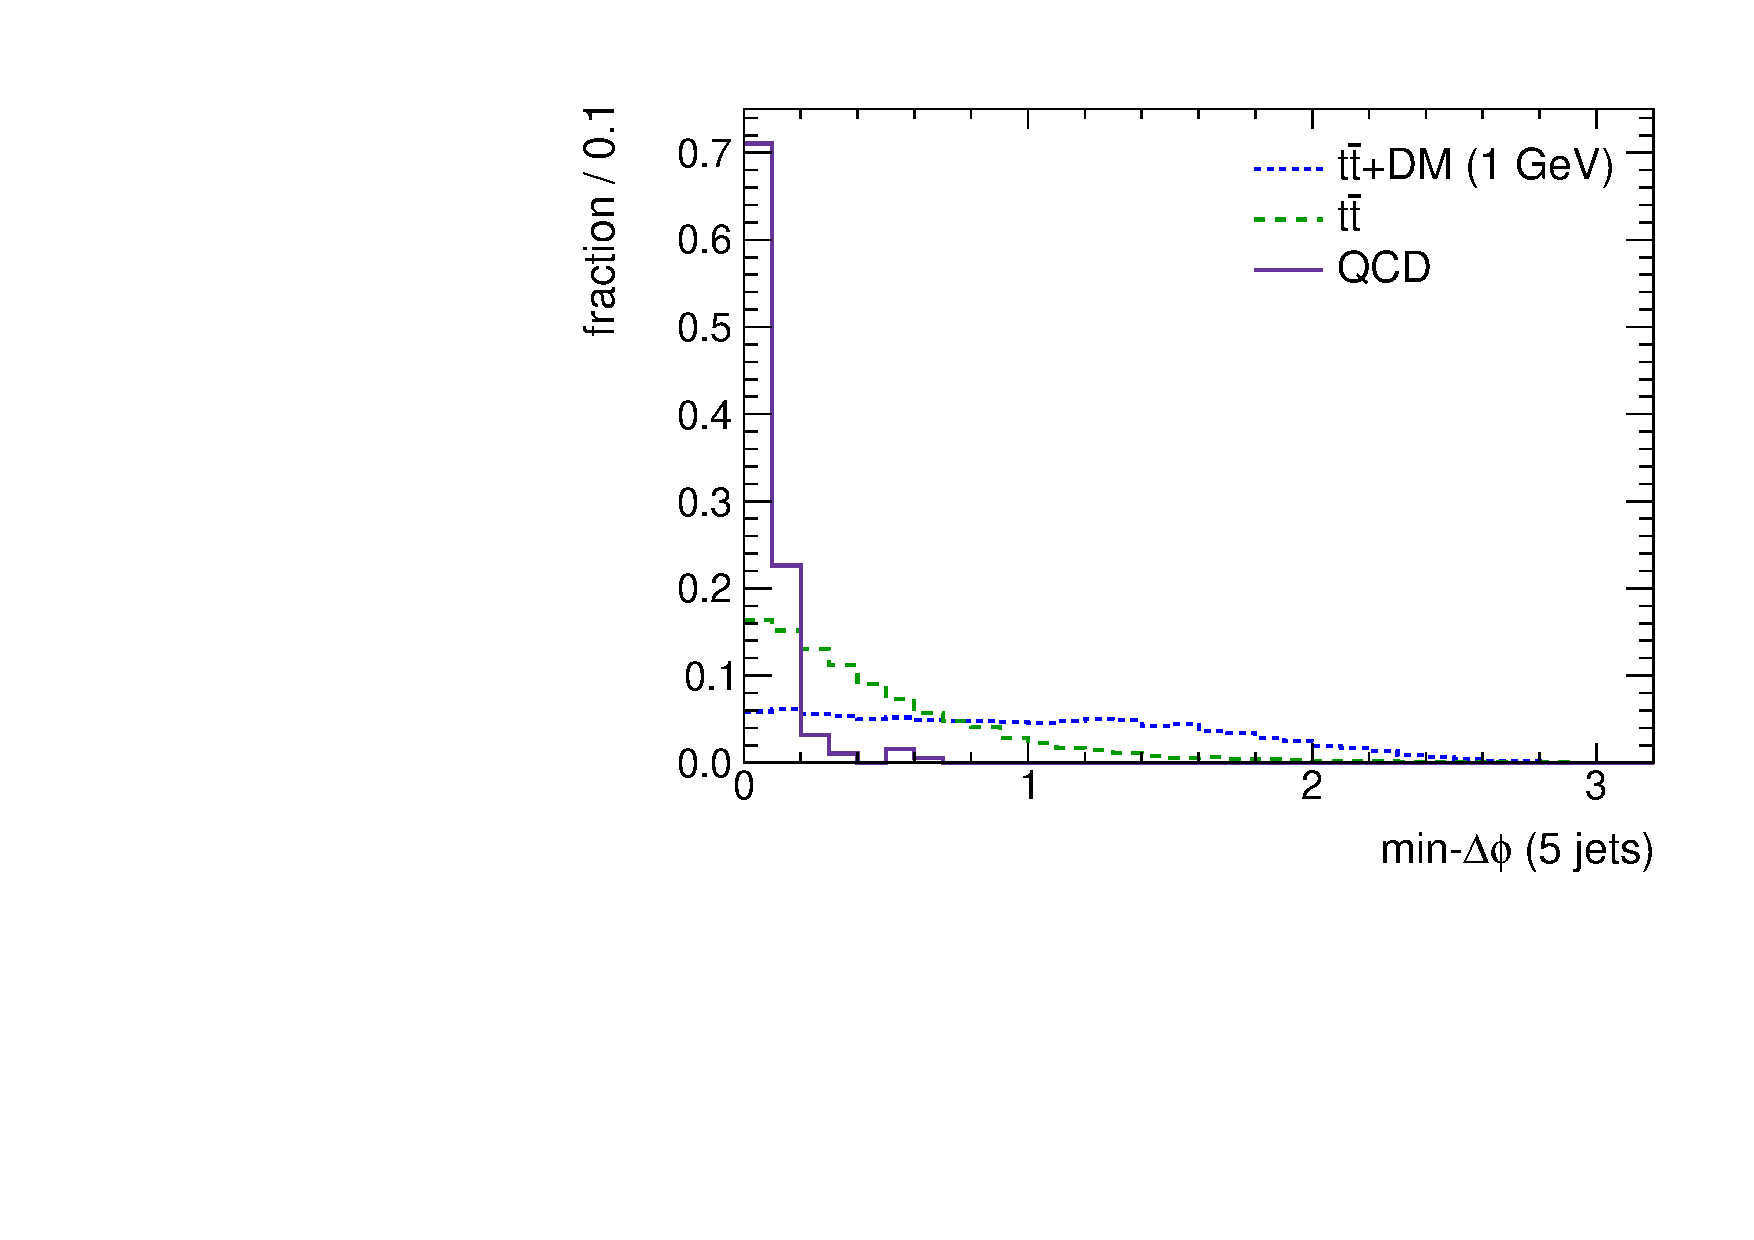
\includegraphics[width=0.32\textwidth]{figures/hadronic-overlay-dphijetmet5.pdf}
  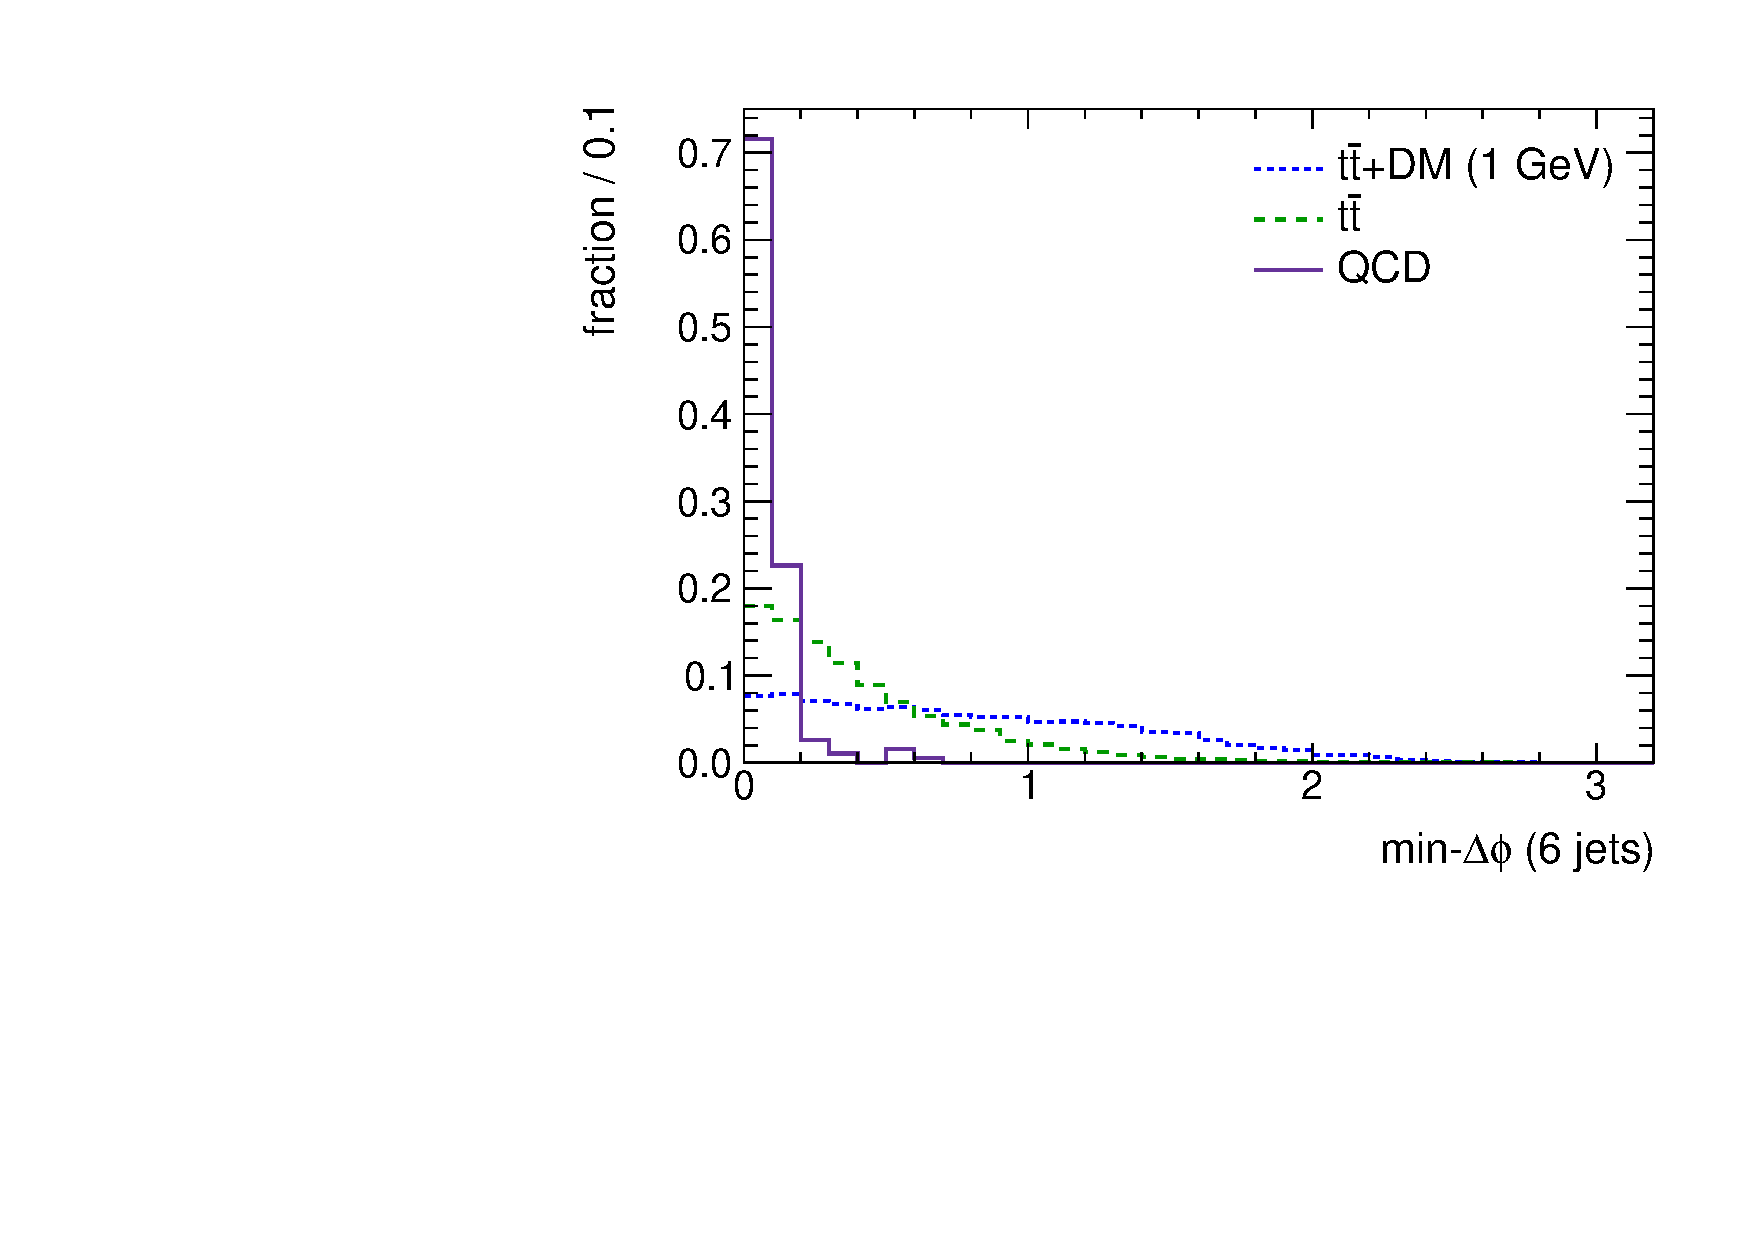
\includegraphics[width=0.32\textwidth]{figures/hadronic-overlay-dphijetmet6.pdf}
  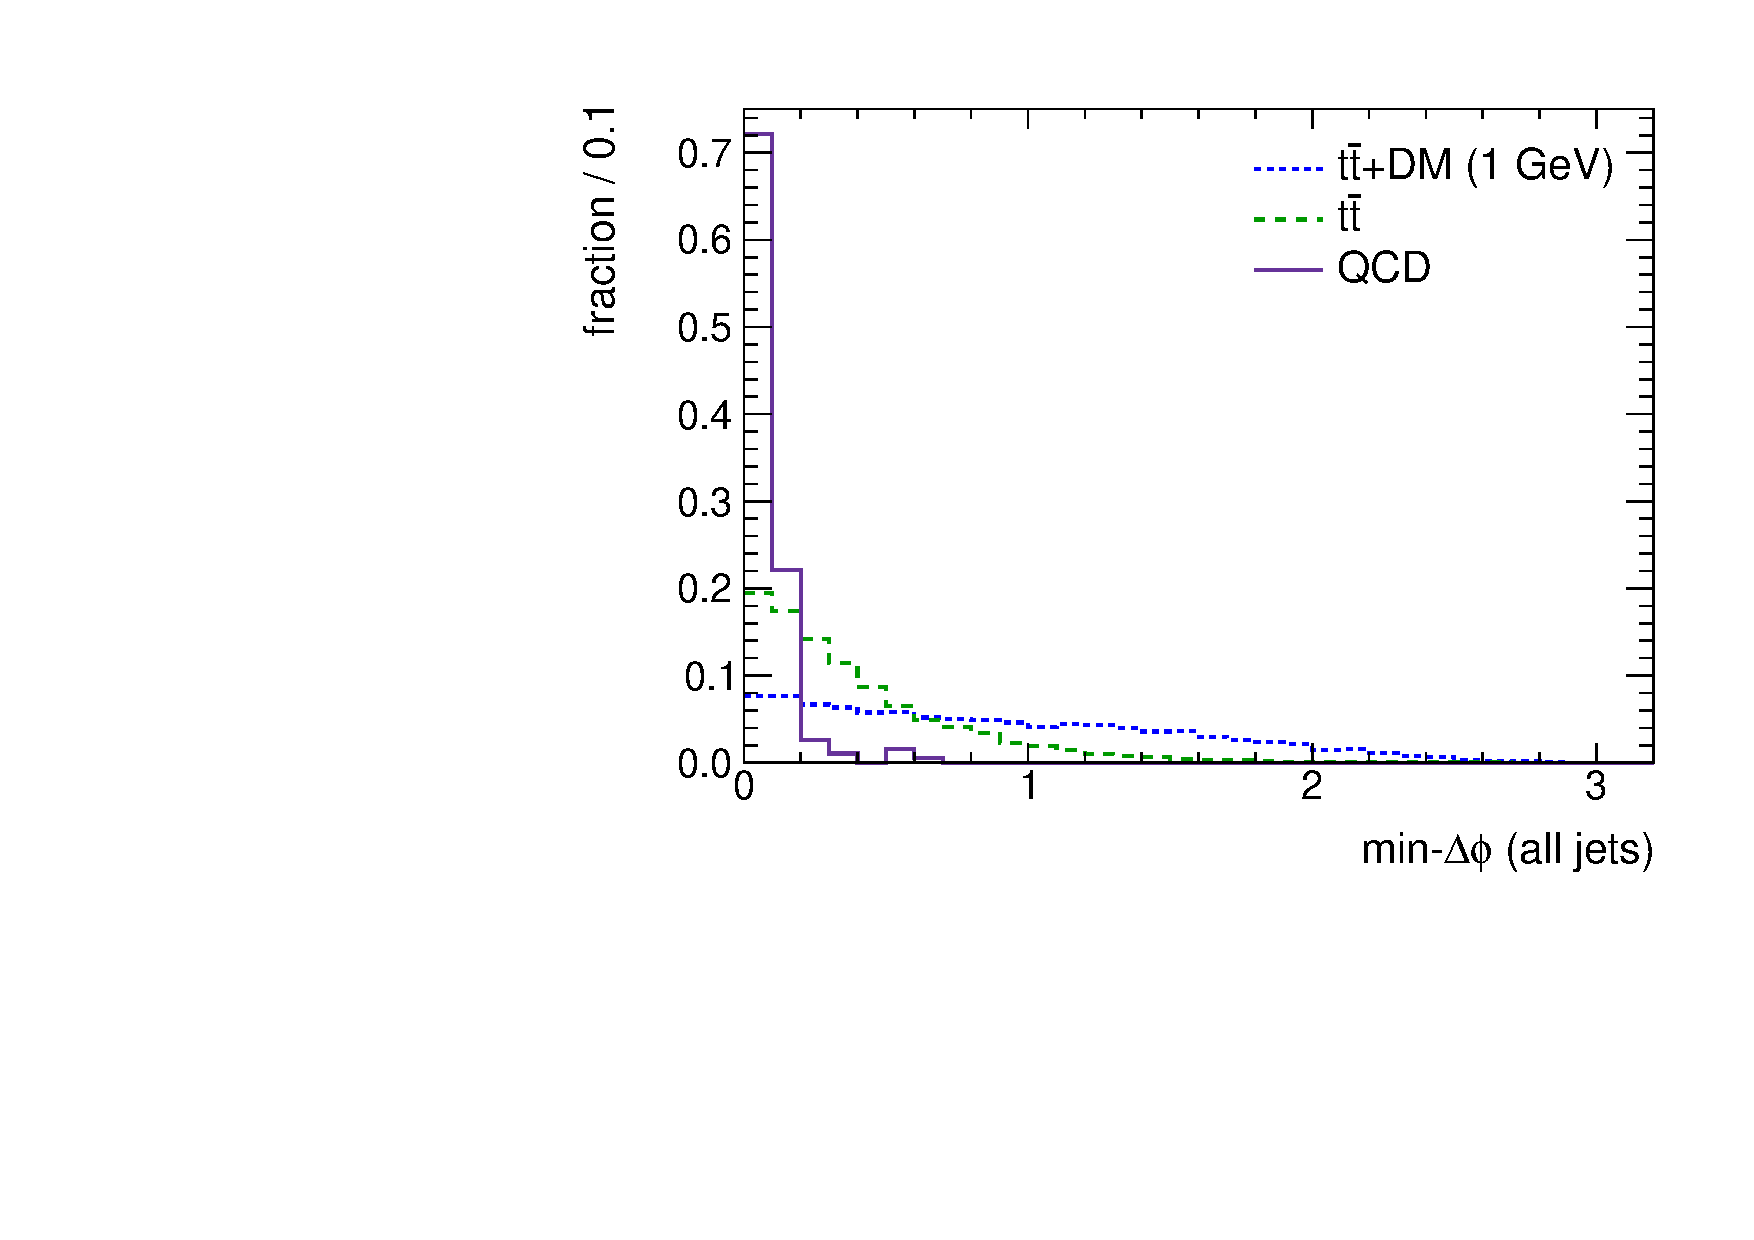
\includegraphics[width=0.32\textwidth]{figures/hadronic-overlay-dphijetmet.pdf}
  \caption{$\Delta\phi$ distributions for QCD, $\ttbar$, and $\ttbar+$DM signal ($M_\chi = 1\:\GeV$). Histograms are normalized to unit area.}
  \label{fig:hadronic_overlay_dphijetmet}
\end{figure}

Including more jets in computing $\Delta\phi$ allows to easily reduce QCD to negligible levels. This is desirable given that it is difficult to define a reliable control region for QCD and MC samples tend to be statistically limited. The performance of the different $\Delta\phi$ definitions are summarized in background versus signal efficiency curves for QCD and $\ttbar$ shown in Fig.~\ref{fig:hadronic_dphijetmet_roc}. Computing the minimum $\Delta\phi$ using up to the sixth leading jet shows the best performance. Note that the definition using all jets performs slightly worse. It will be important to revisit these defintions again with data and more realistic MC samples.

\begin{figure}[htbp]
  \centering
  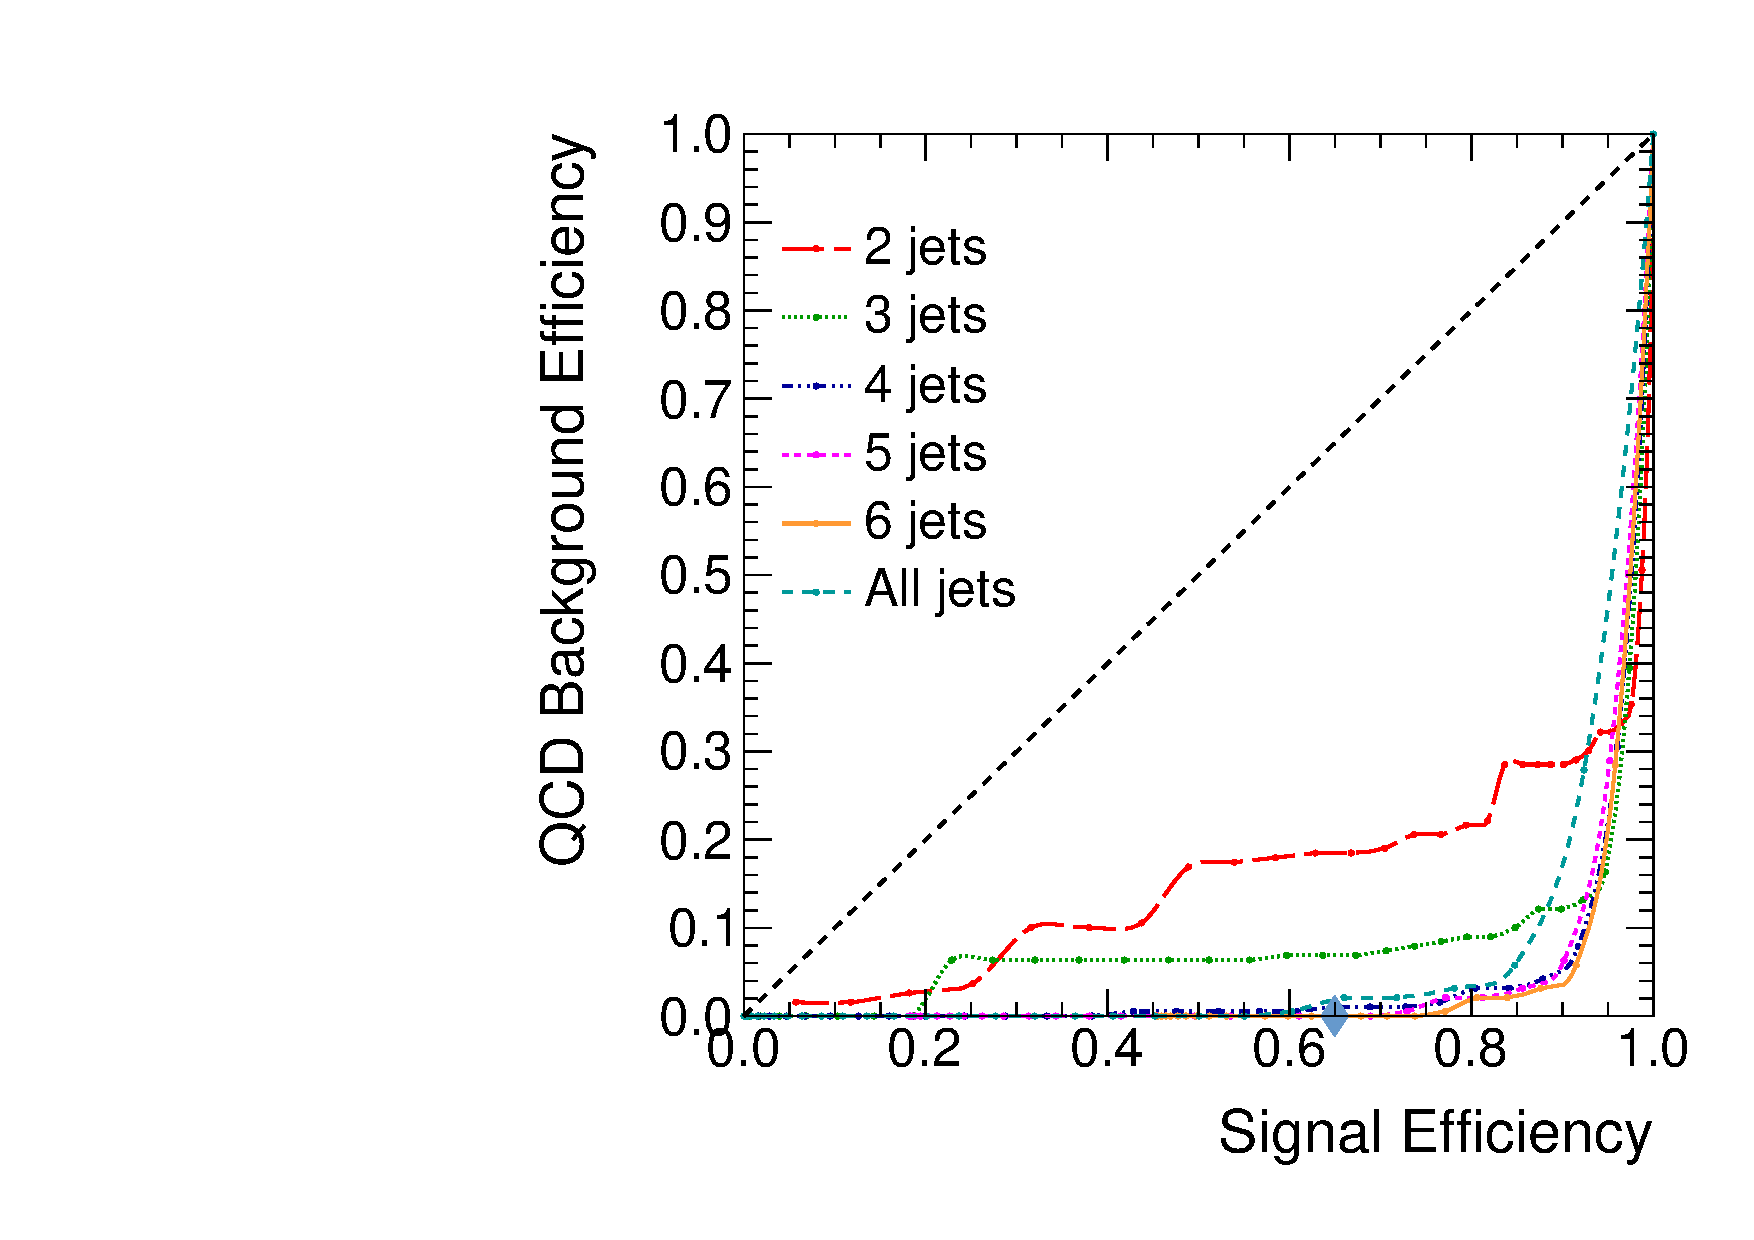
\includegraphics[width=0.32\textwidth]{figures/ttdm1_vs_qcd-hadronic-roc.pdf}
  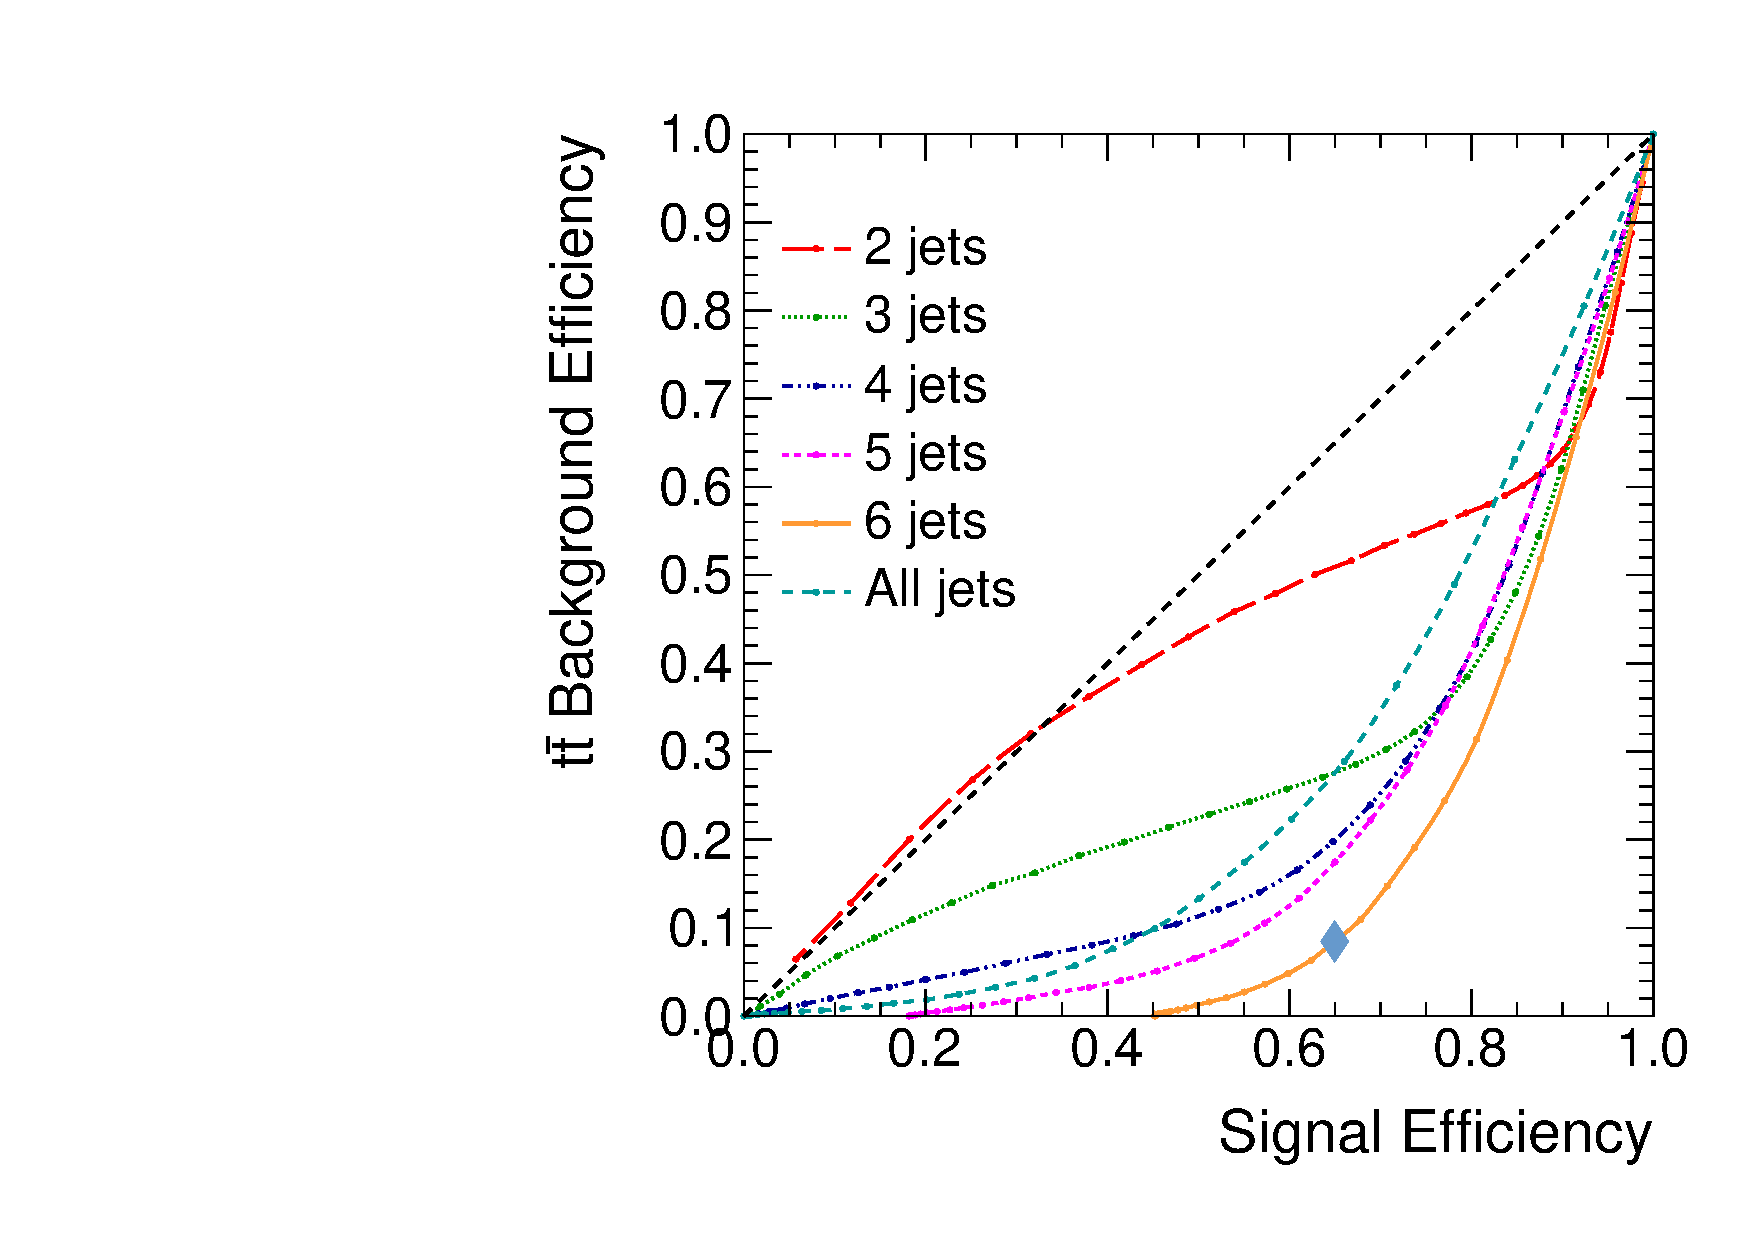
\includegraphics[width=0.32\textwidth]{figures/ttdm1_vs_ttbar-hadronic-roc.pdf}
  \caption{Background versus signal efficiency curves for various $\Delta\phi$ definitions. The diamond marker indicates the operating point corresponding to the $\min_{i=1,\ldots,6}\Delta\phi\left(j_i,\met\right)$ cut used in the inclusive hadronic selection.}
  \label{fig:hadronic_dphijetmet_roc}
\end{figure}

\subsection{Semileptonic channel}
In the semileptonic channel, the $\Delta\phi$ variable provides a handle to further reduce the dileptonic $\ttbar$ background. Definitions of $\Delta\phi$ using up to the second, third, fourth leading jets, and all jets, were investigated. All other cuts from the inclusive semileptonic selection are applied. The distributions for these definitions are shown for all processes in Fig.~\ref{fig:semilept_dphijetmet} and Fig.~\ref{fig:semilept_dphijetmetlog}, and the shapes between QCD, $\ttbar$, and signal are compared in Fig.~\ref{fig:semilept_overlay_dphijetmet}.

\begin{figure}[htbp]
  \centering
  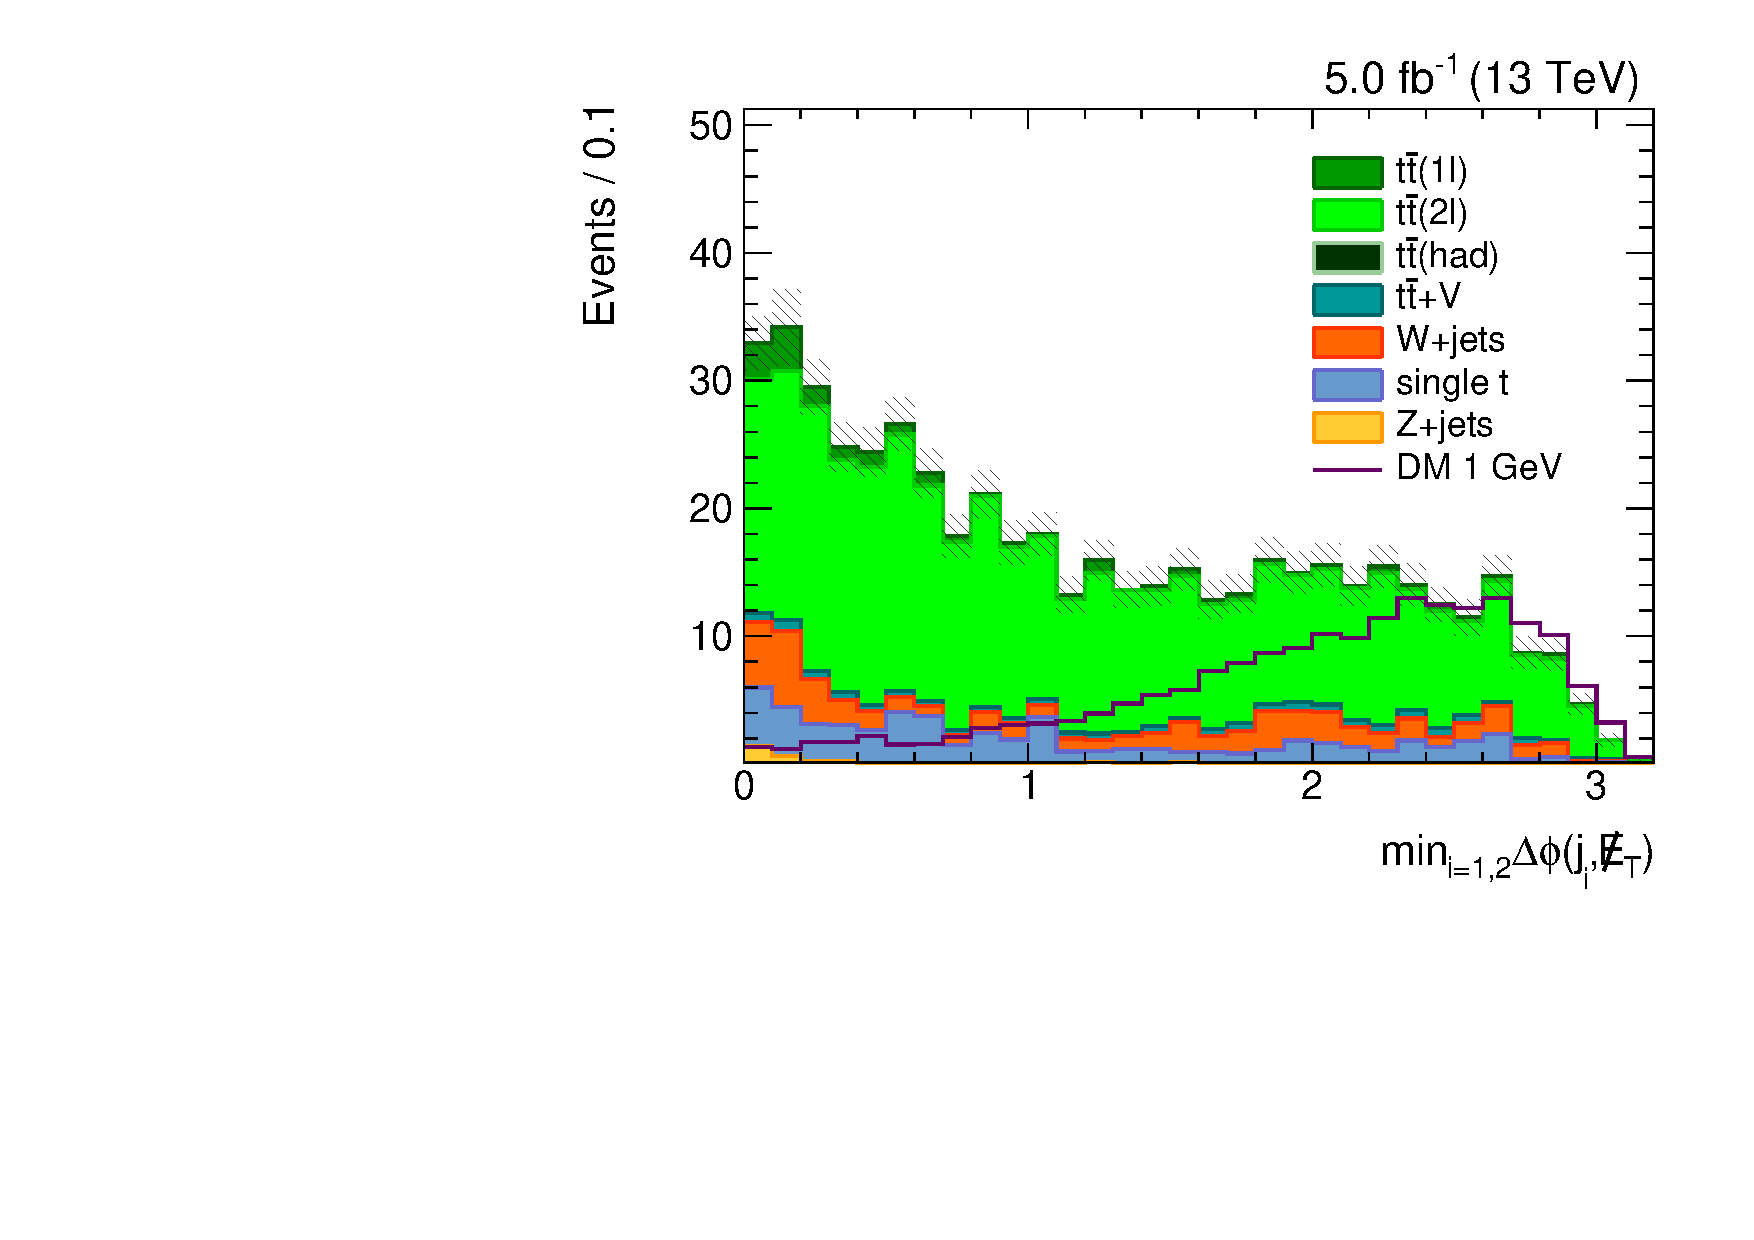
\includegraphics[width=0.48\textwidth]{figures/semilept-incl-dphijetmet2_l.pdf}
  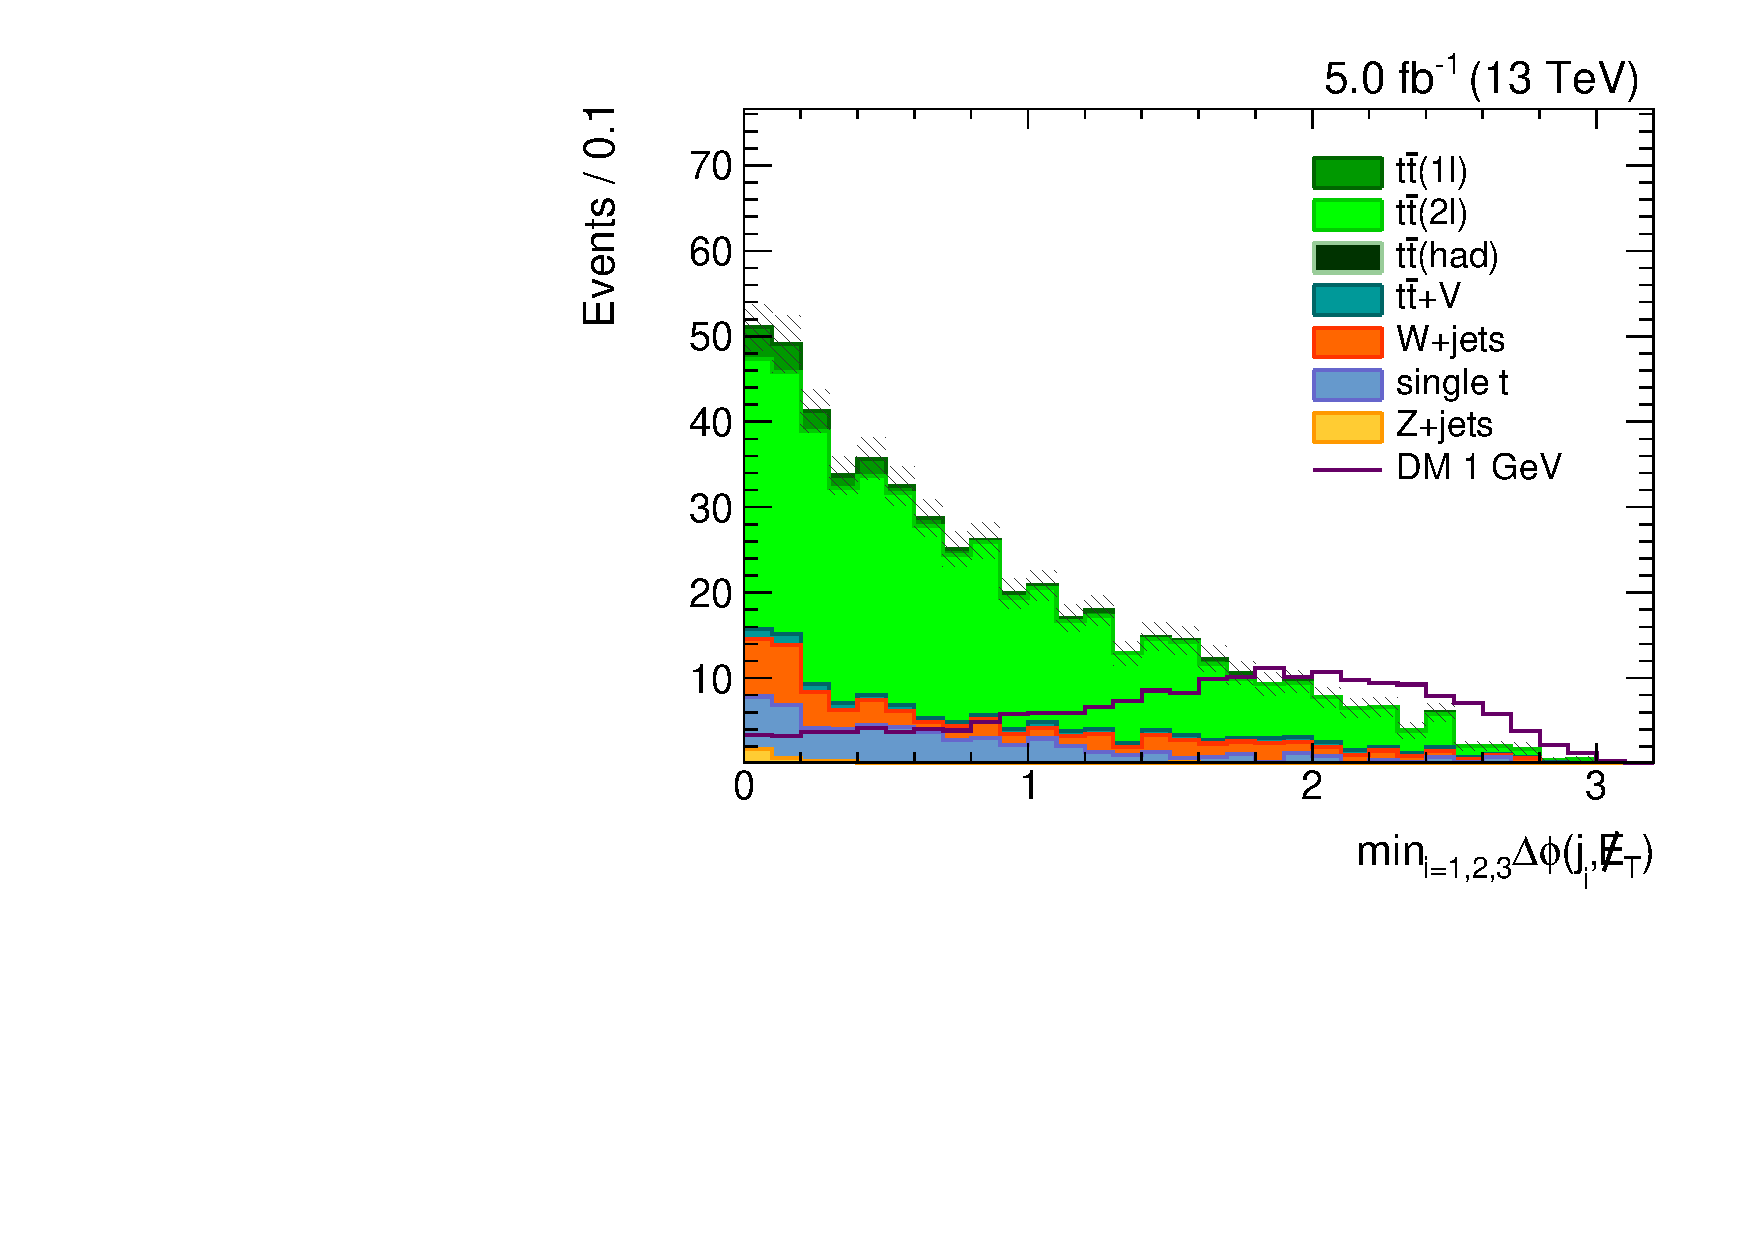
\includegraphics[width=0.48\textwidth]{figures/semilept-incl-dphijetmet3_l.pdf} \\
  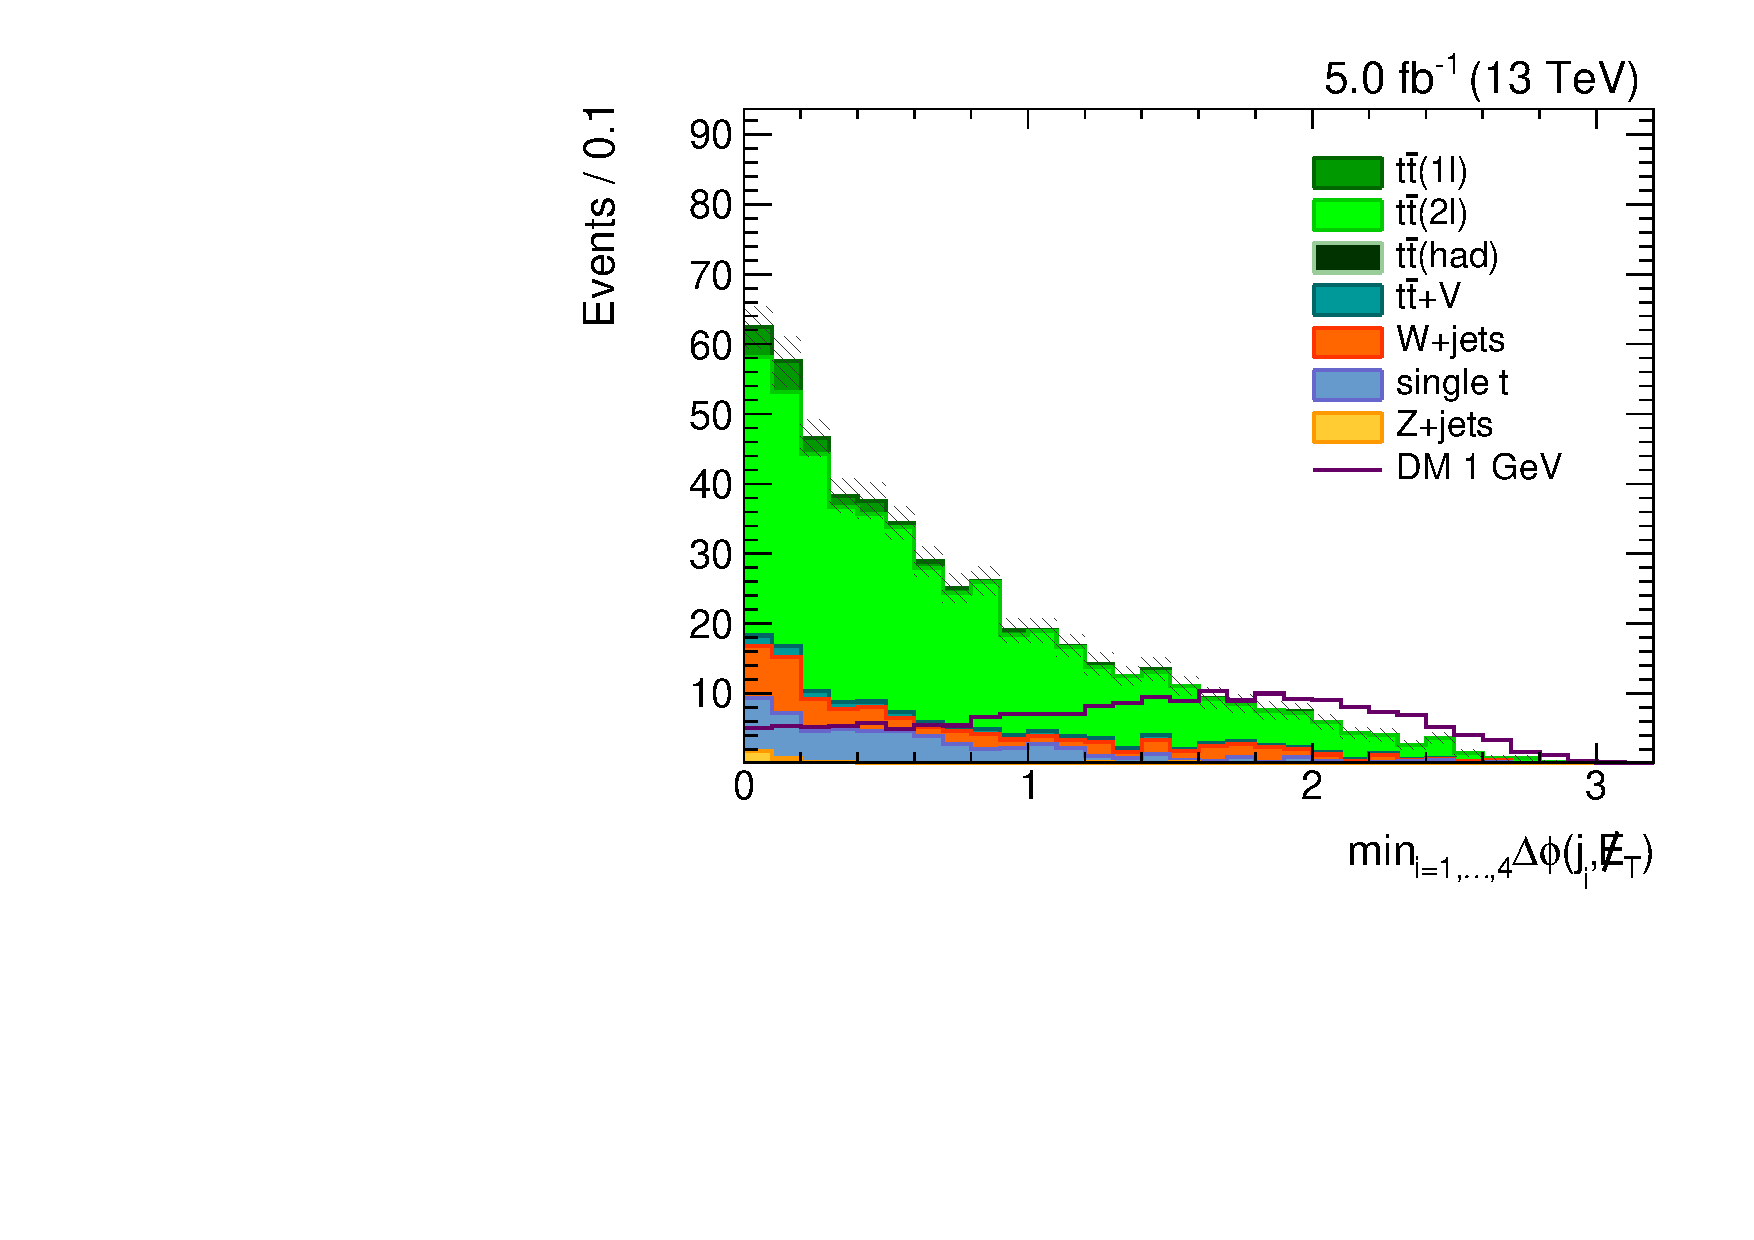
\includegraphics[width=0.48\textwidth]{figures/semilept-incl-dphijetmet4_l.pdf}
  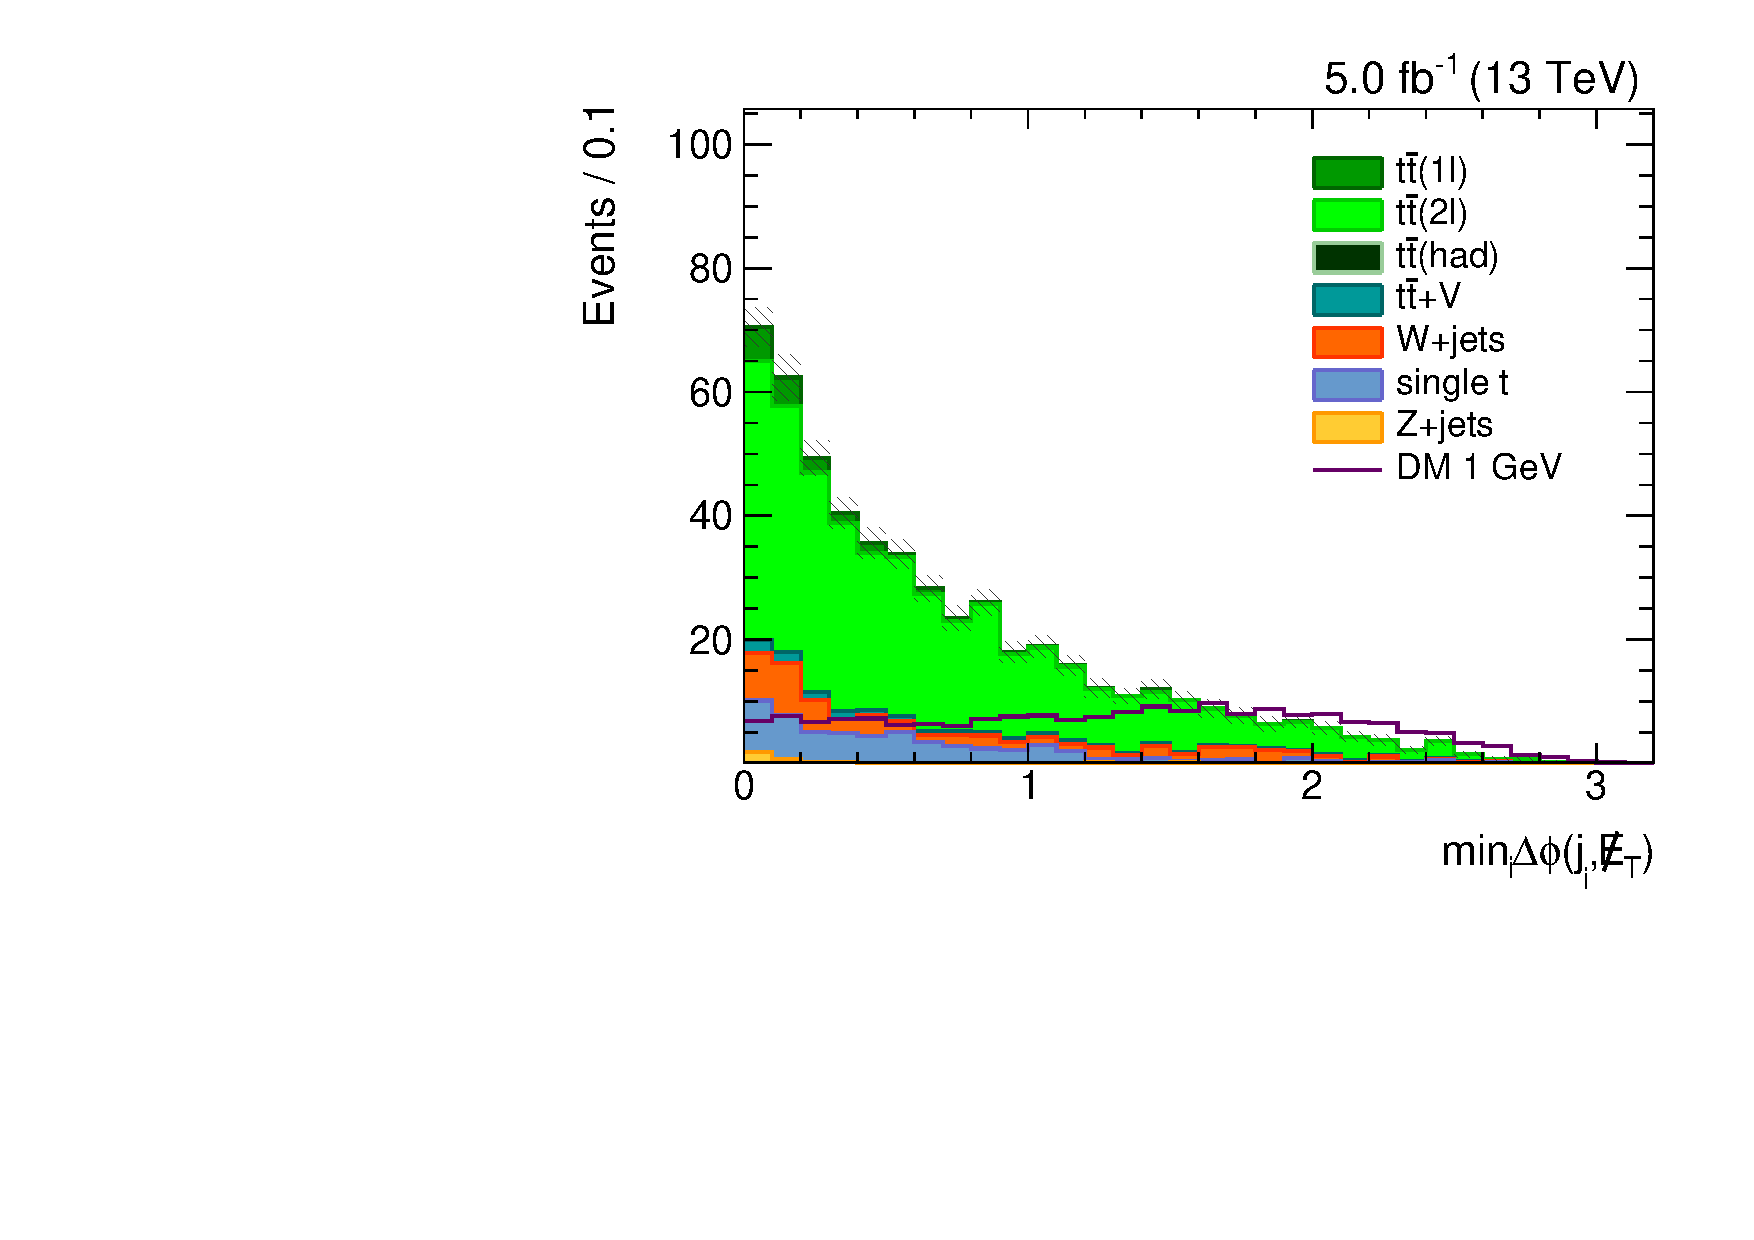
\includegraphics[width=0.48\textwidth]{figures/semilept-incl-dphijetmet_l.pdf}
  \caption{$\Delta\phi$ distributions for various definitions.}
  \label{fig:semilept_dphijetmet}
\end{figure}

\begin{figure}[htbp]
  \centering
  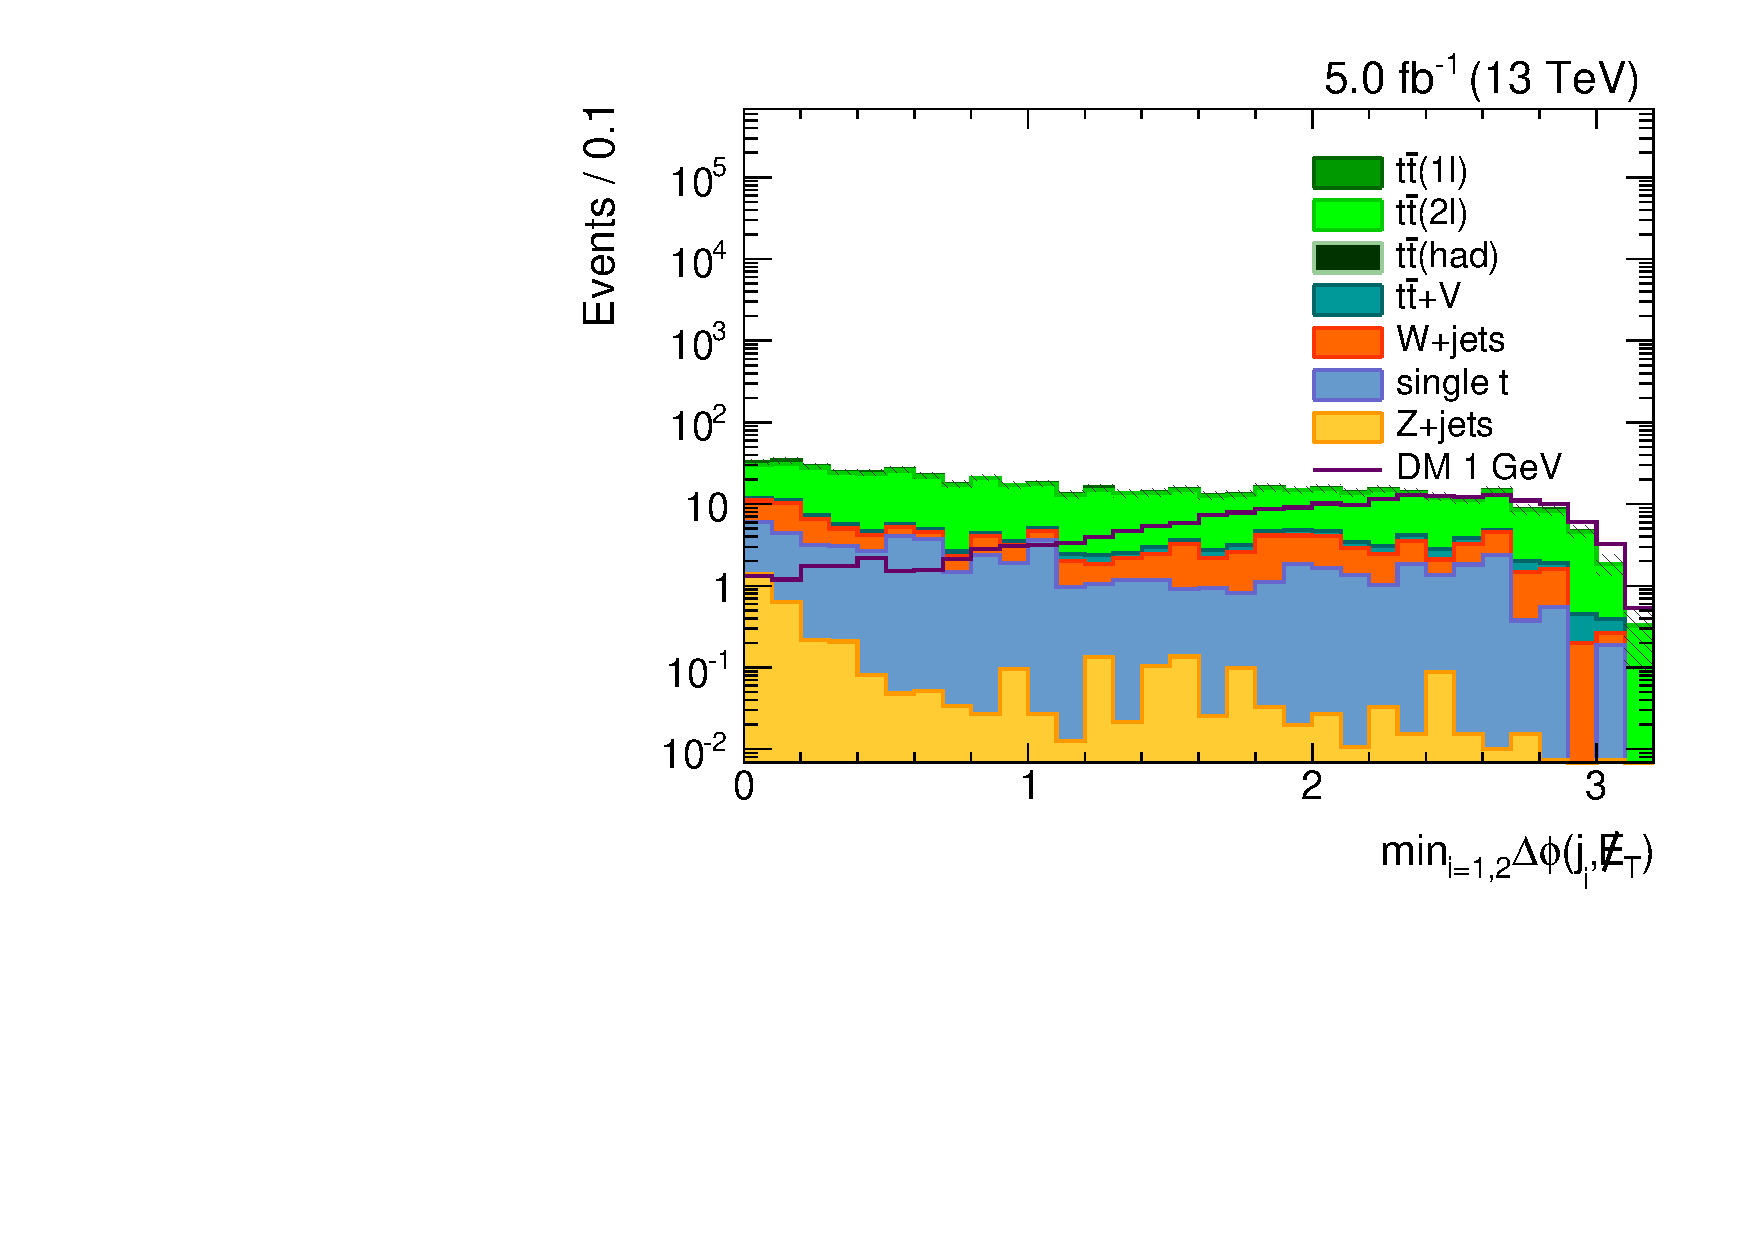
\includegraphics[width=0.48\textwidth]{figures/semilept-incl-dphijetmet2log_l.pdf}
  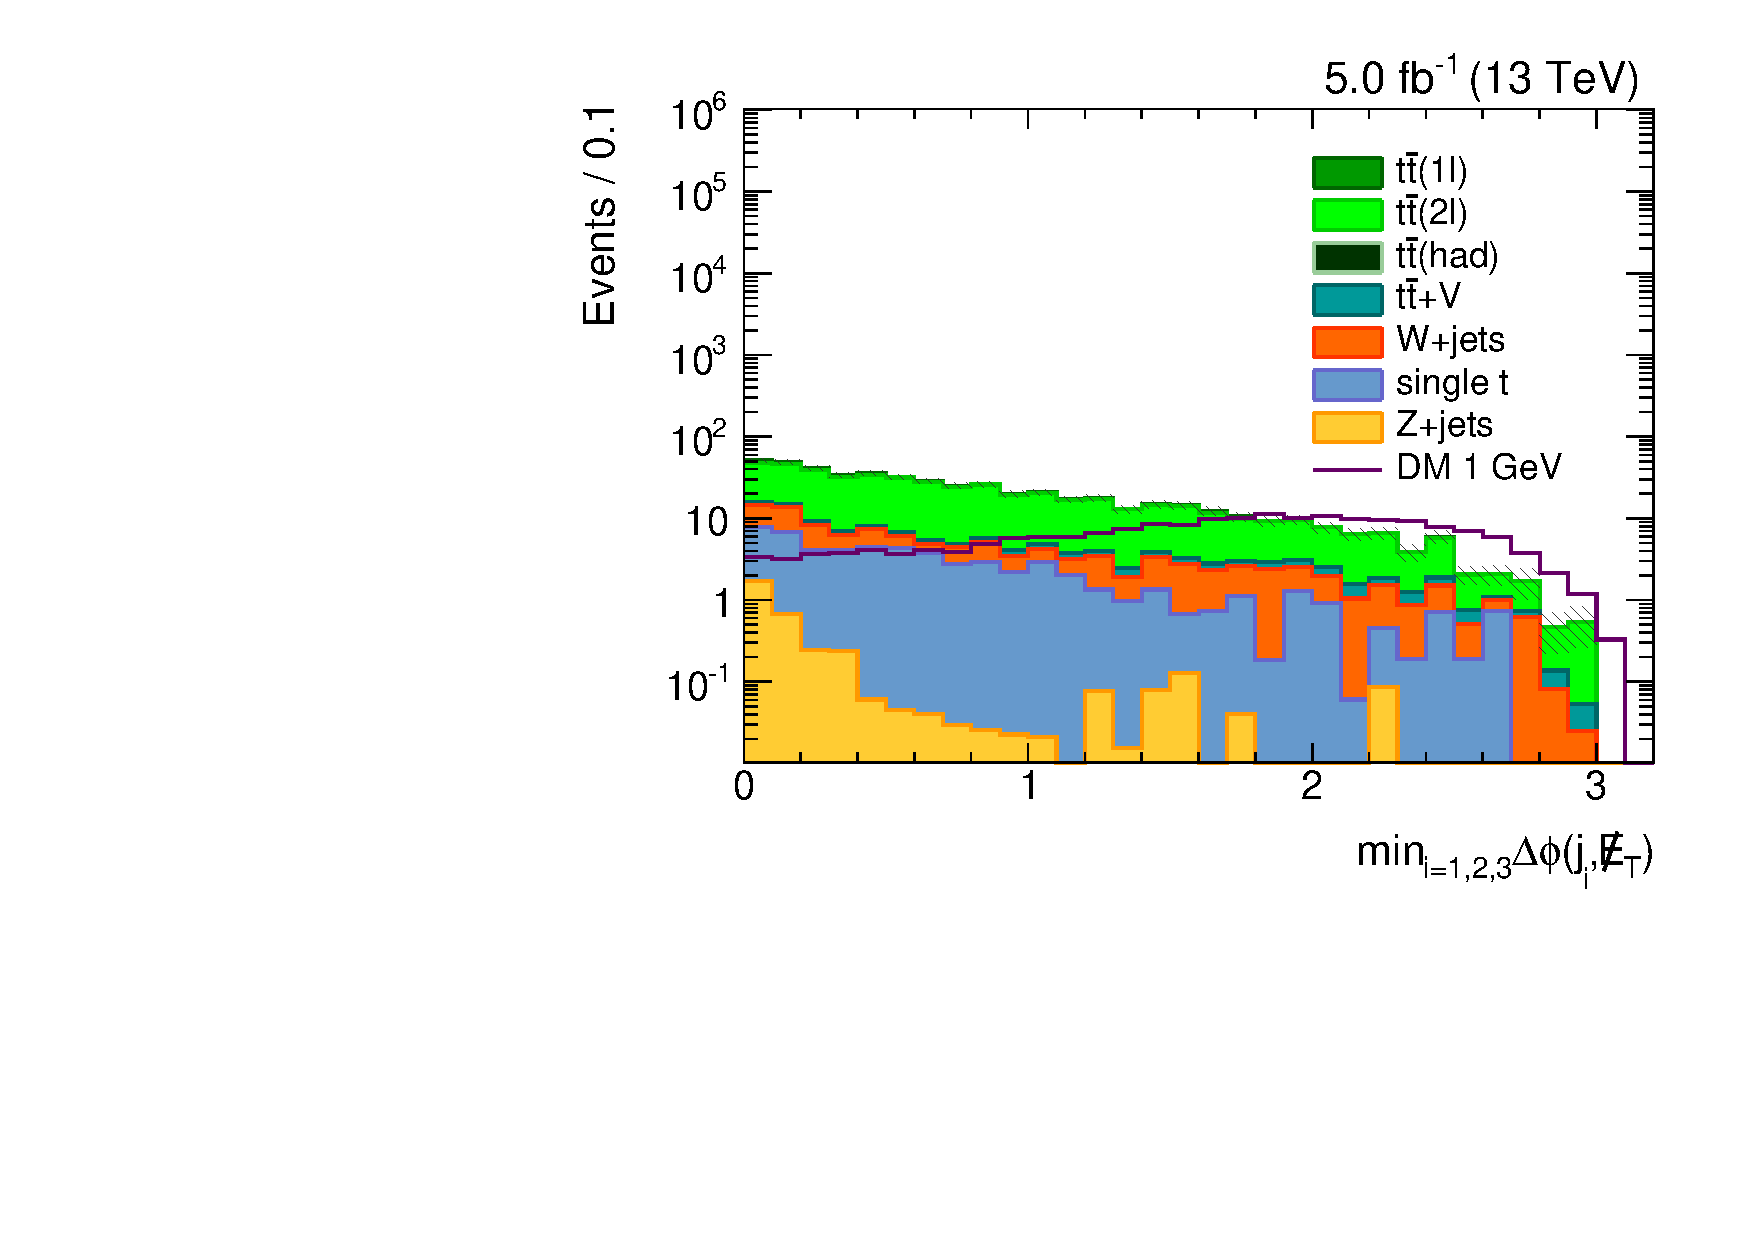
\includegraphics[width=0.48\textwidth]{figures/semilept-incl-dphijetmet3log_l.pdf} \\
  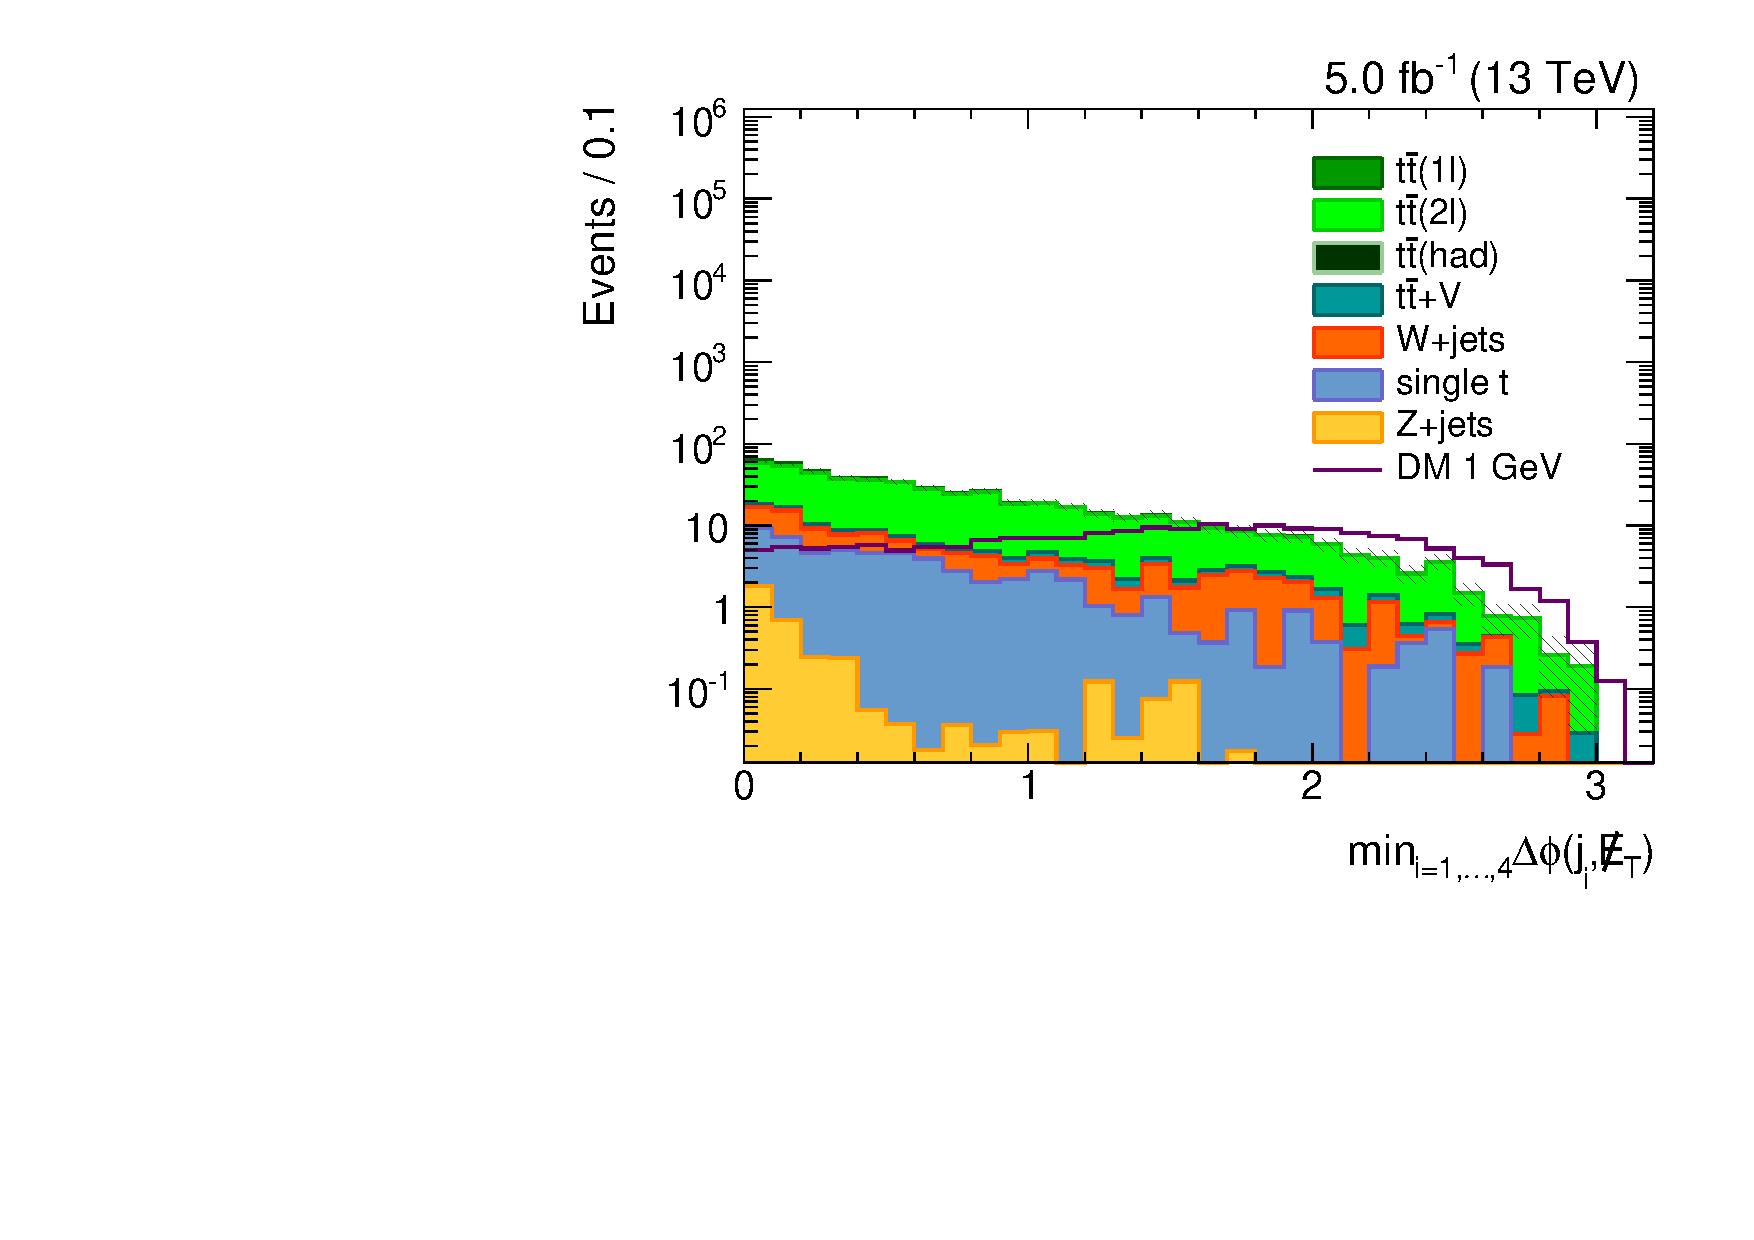
\includegraphics[width=0.48\textwidth]{figures/semilept-incl-dphijetmet4log_l.pdf}
  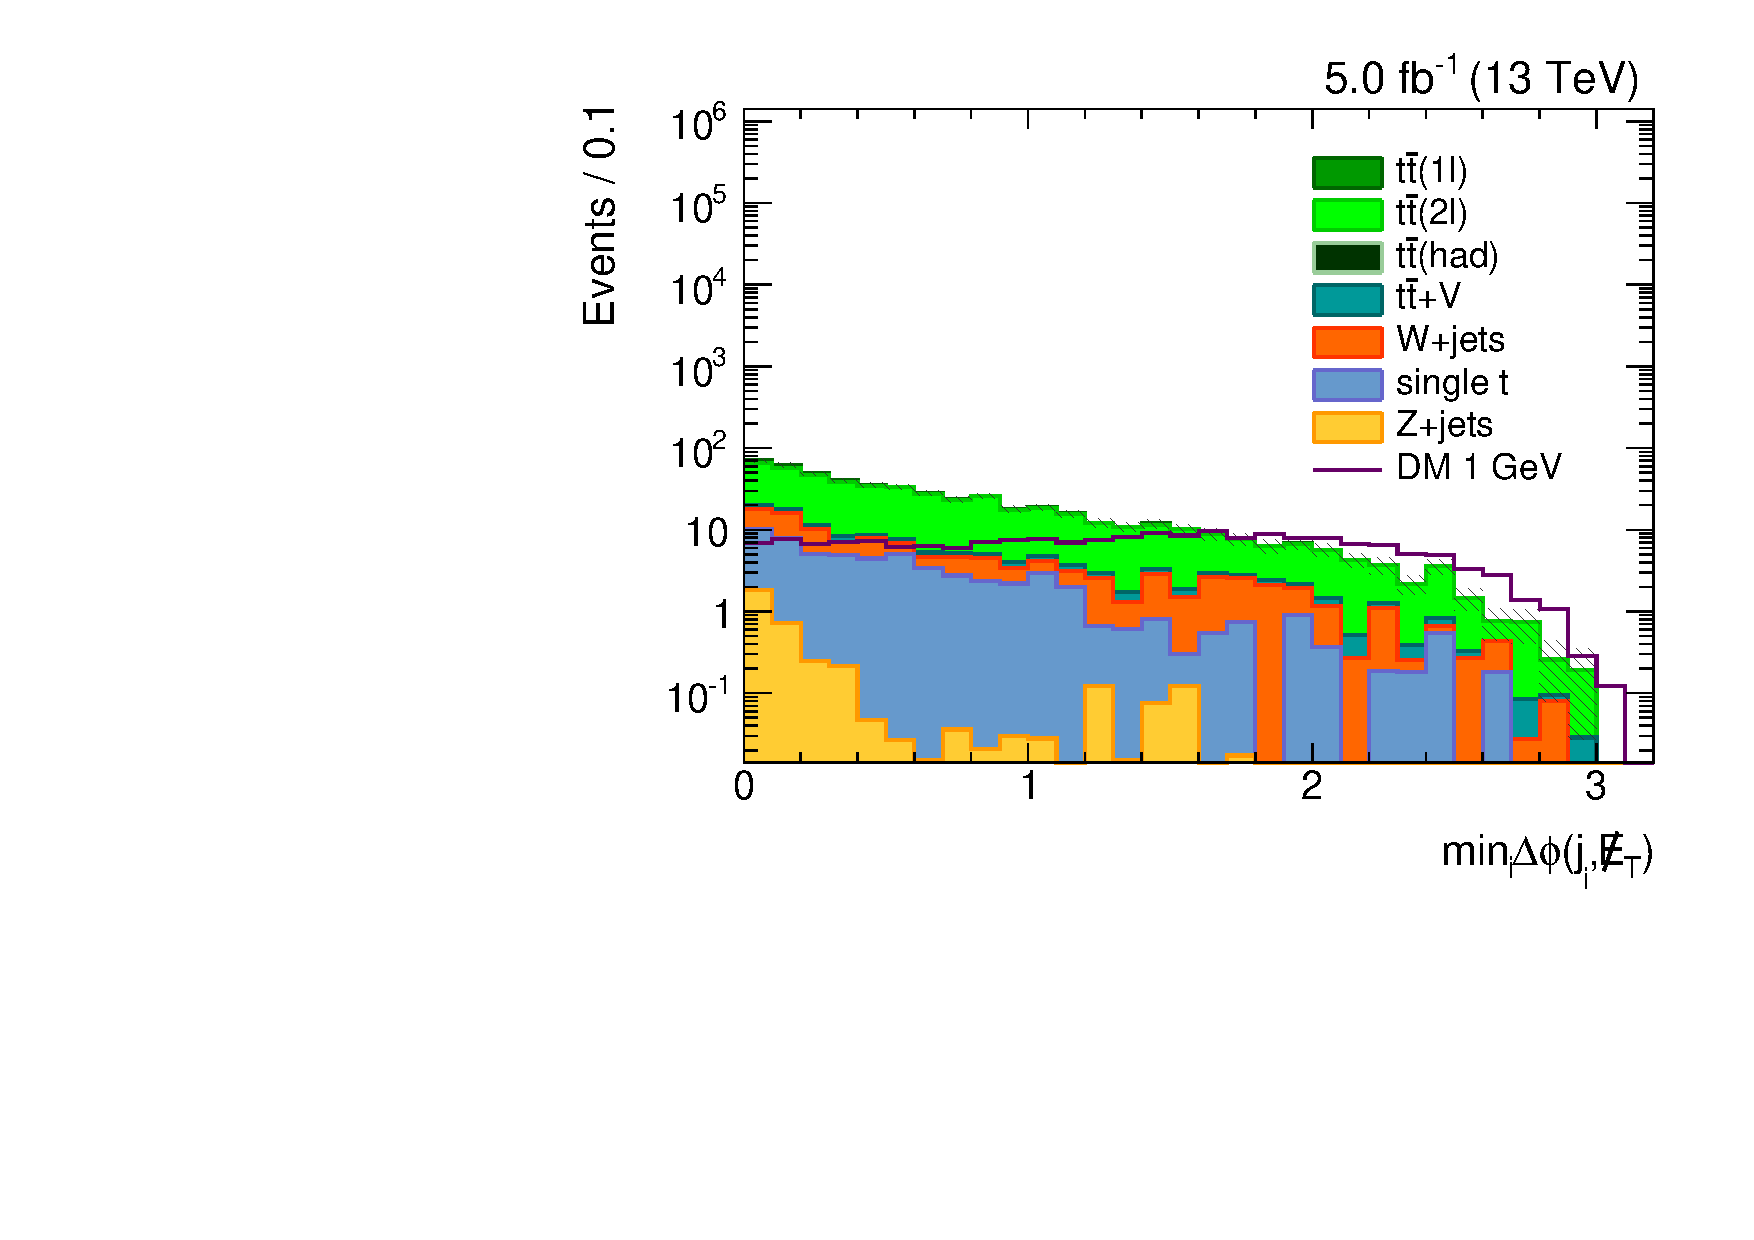
\includegraphics[width=0.48\textwidth]{figures/semilept-incl-dphijetmetlog_l.pdf}
  \caption{$\Delta\phi$ distributions for various definitions in log scale.}
  \label{fig:semilept_dphijetmetlog}
\end{figure}

\begin{figure}[htbp]
  \centering
  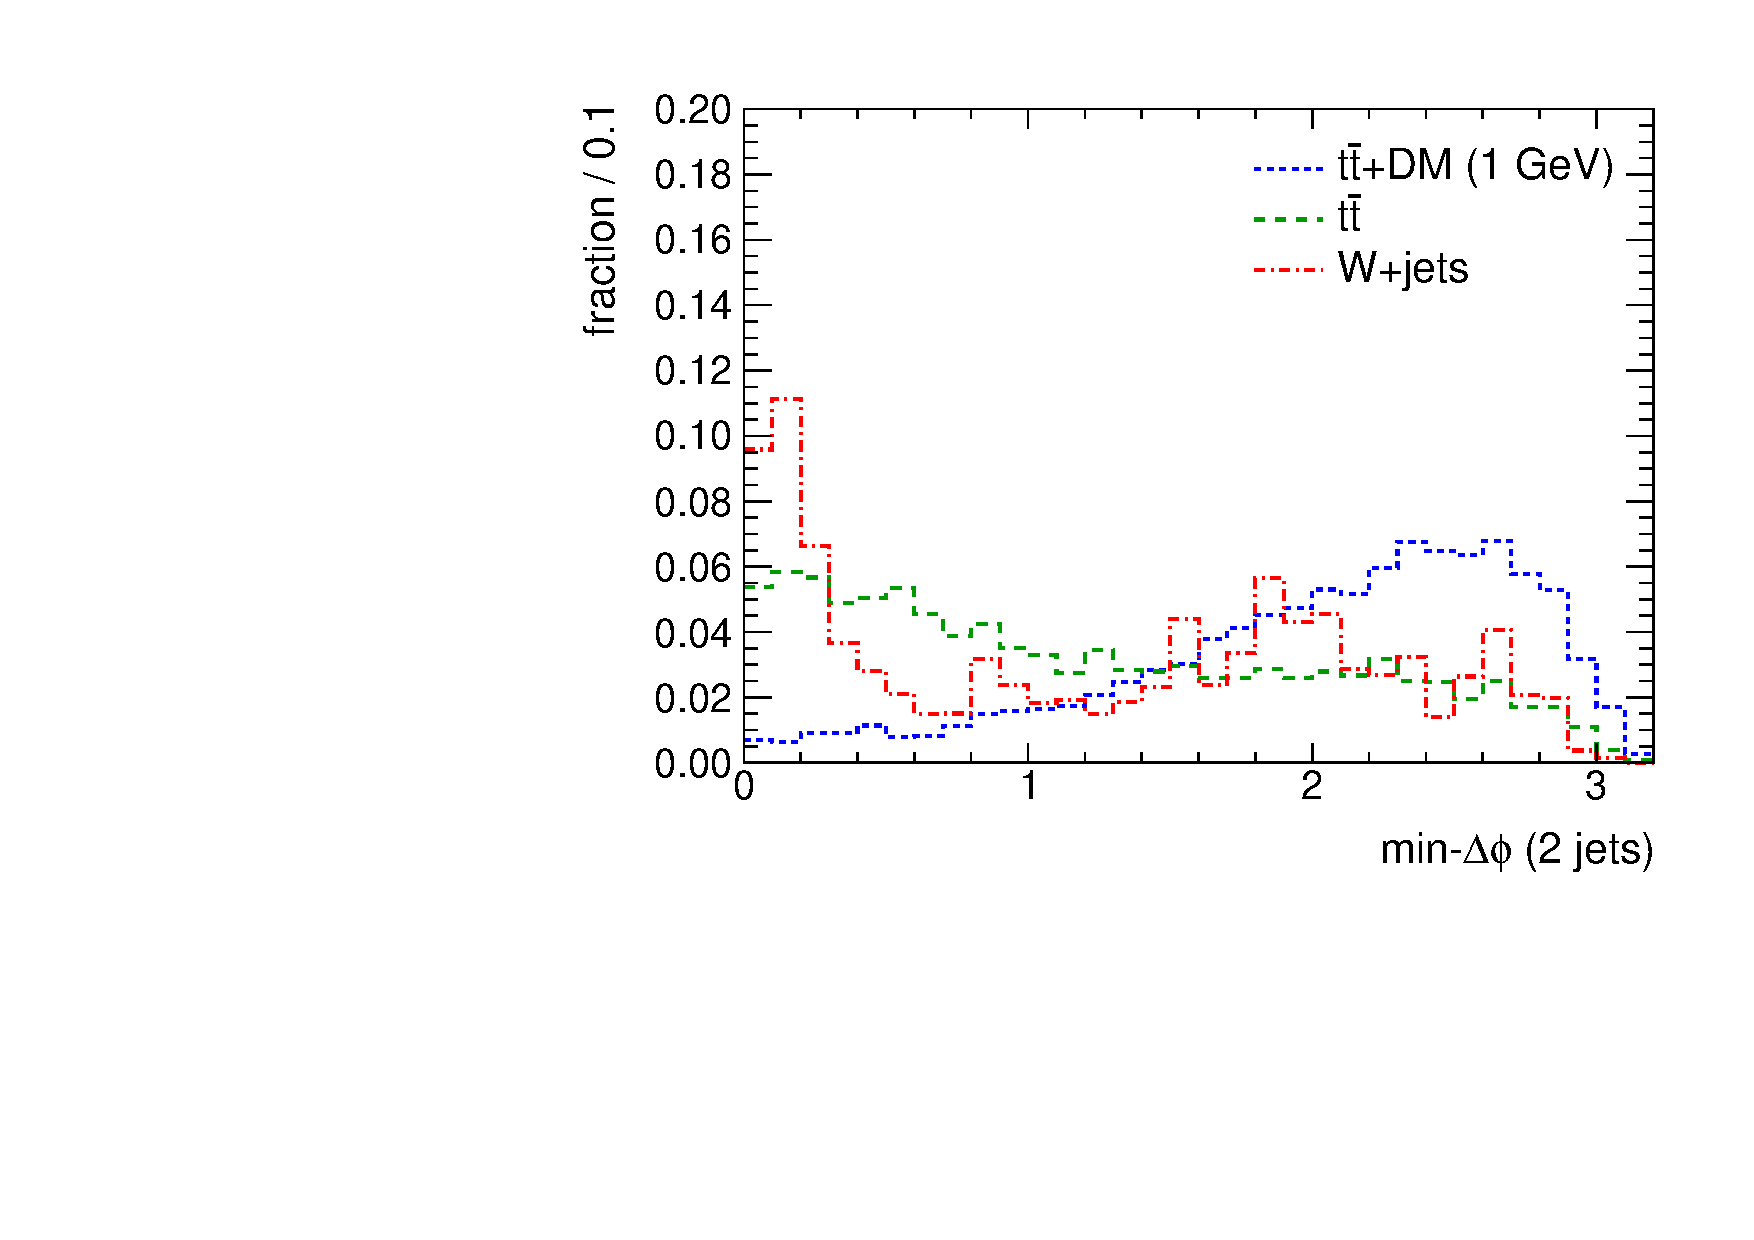
\includegraphics[width=0.32\textwidth]{figures/semilept-overlay-dphijetmet2.pdf}
  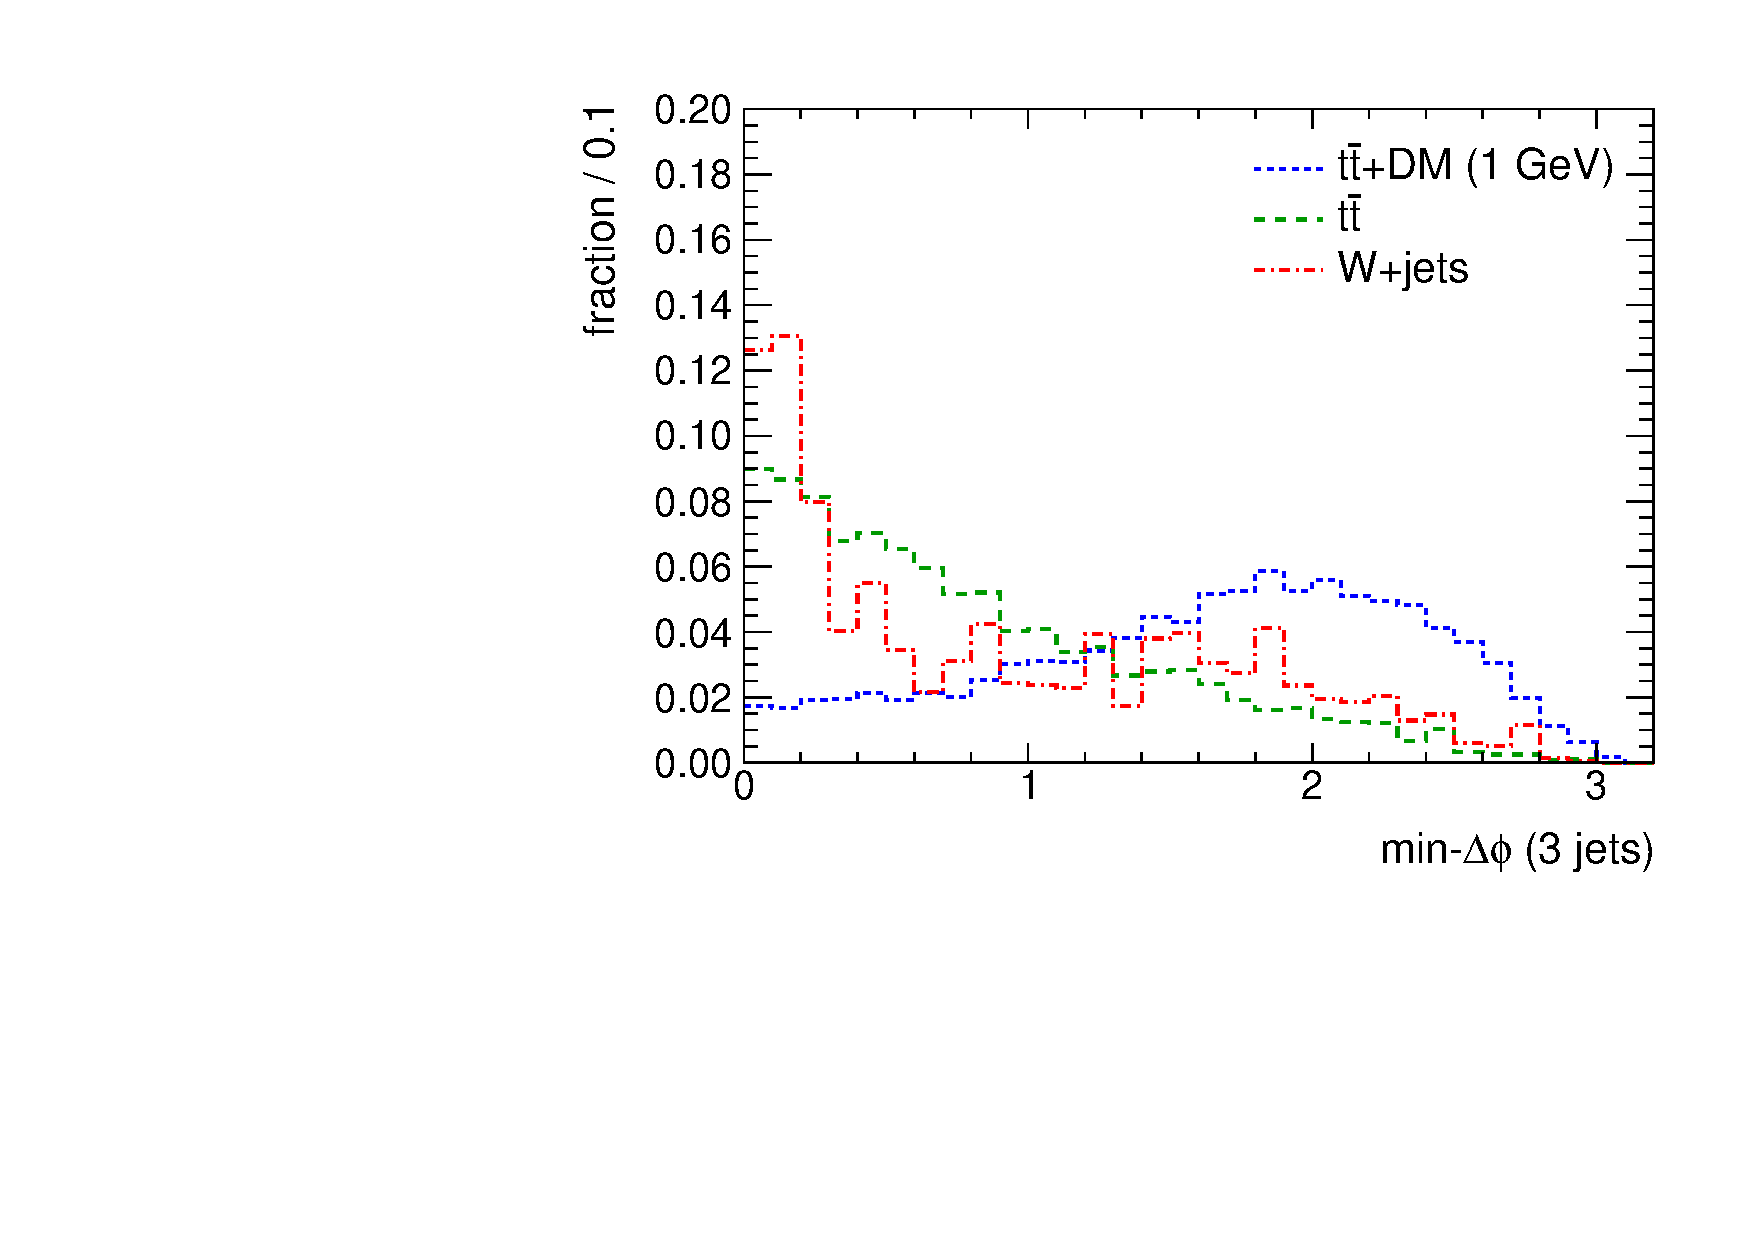
\includegraphics[width=0.32\textwidth]{figures/semilept-overlay-dphijetmet3.pdf} \\
  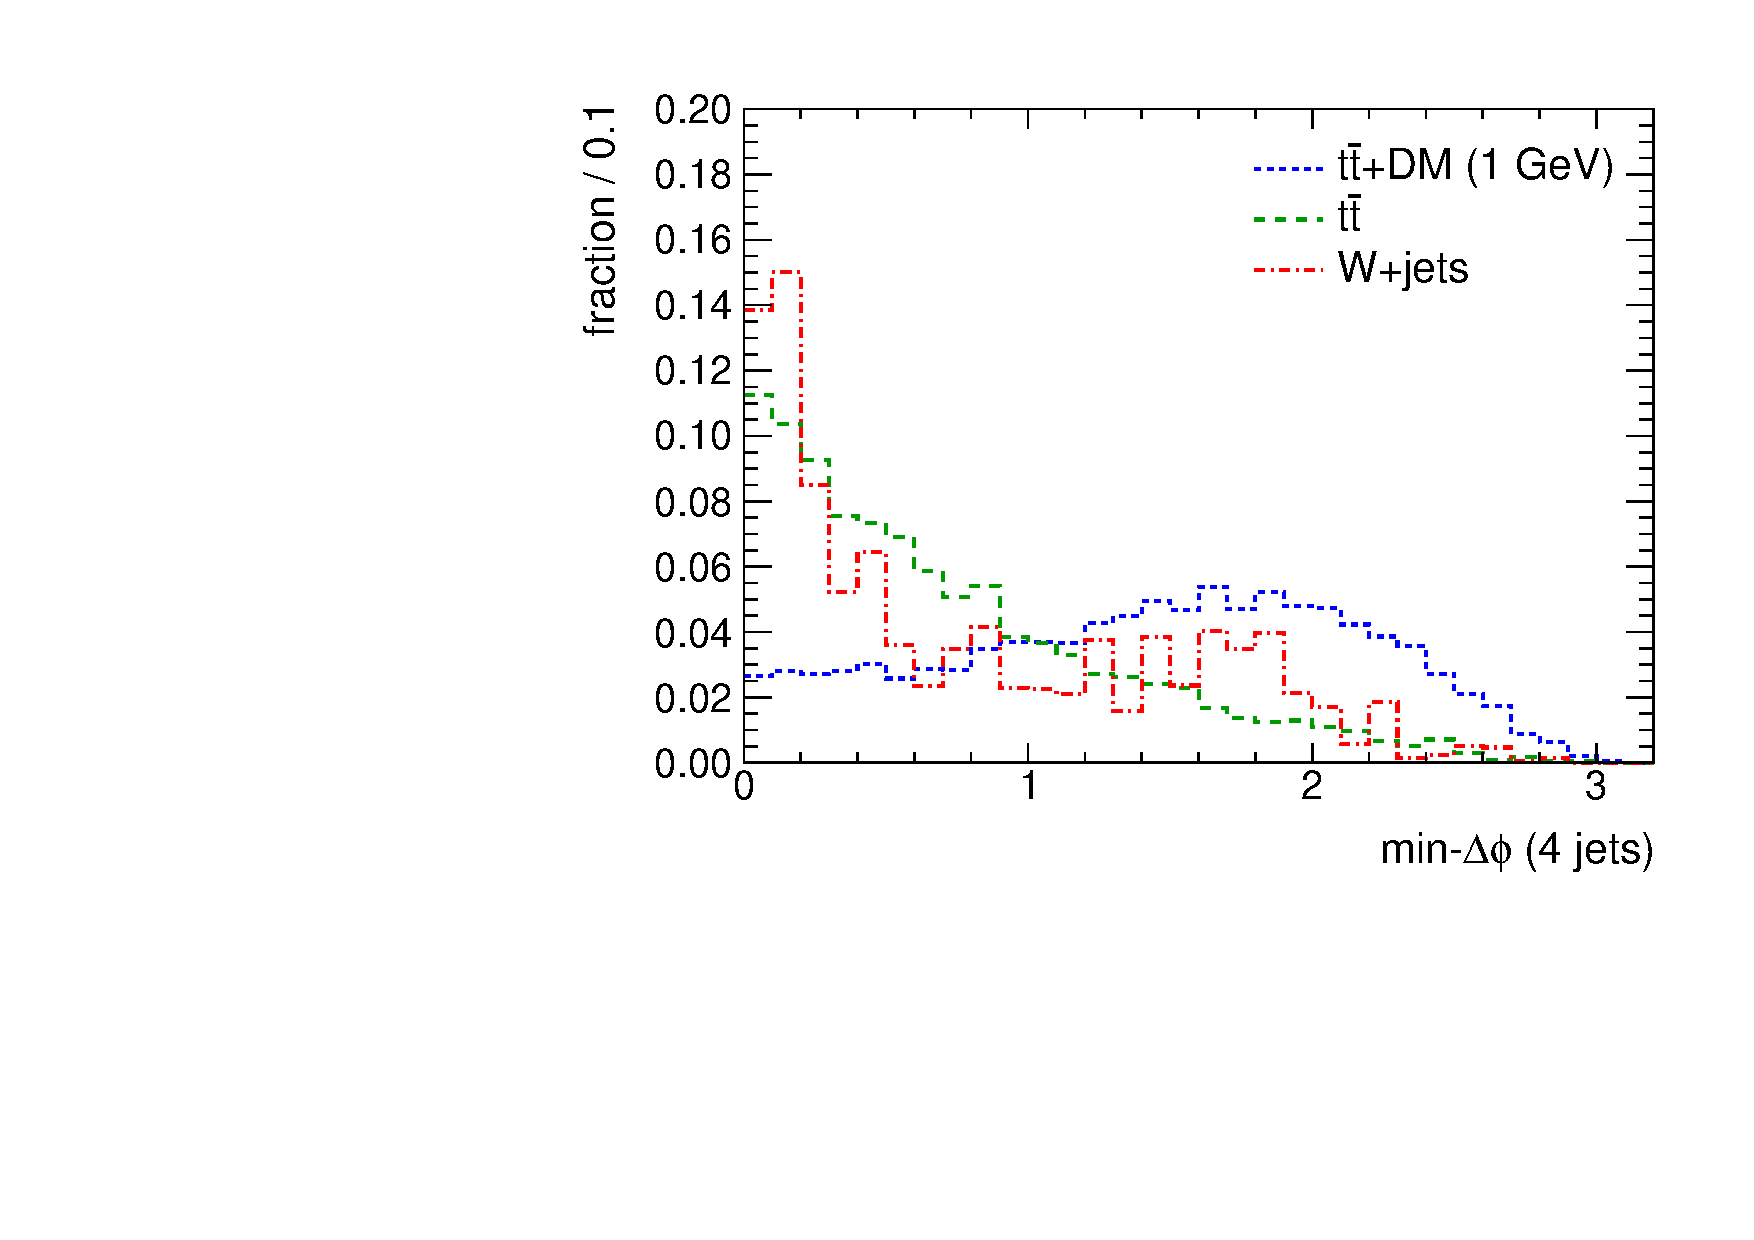
\includegraphics[width=0.32\textwidth]{figures/semilept-overlay-dphijetmet4.pdf}
  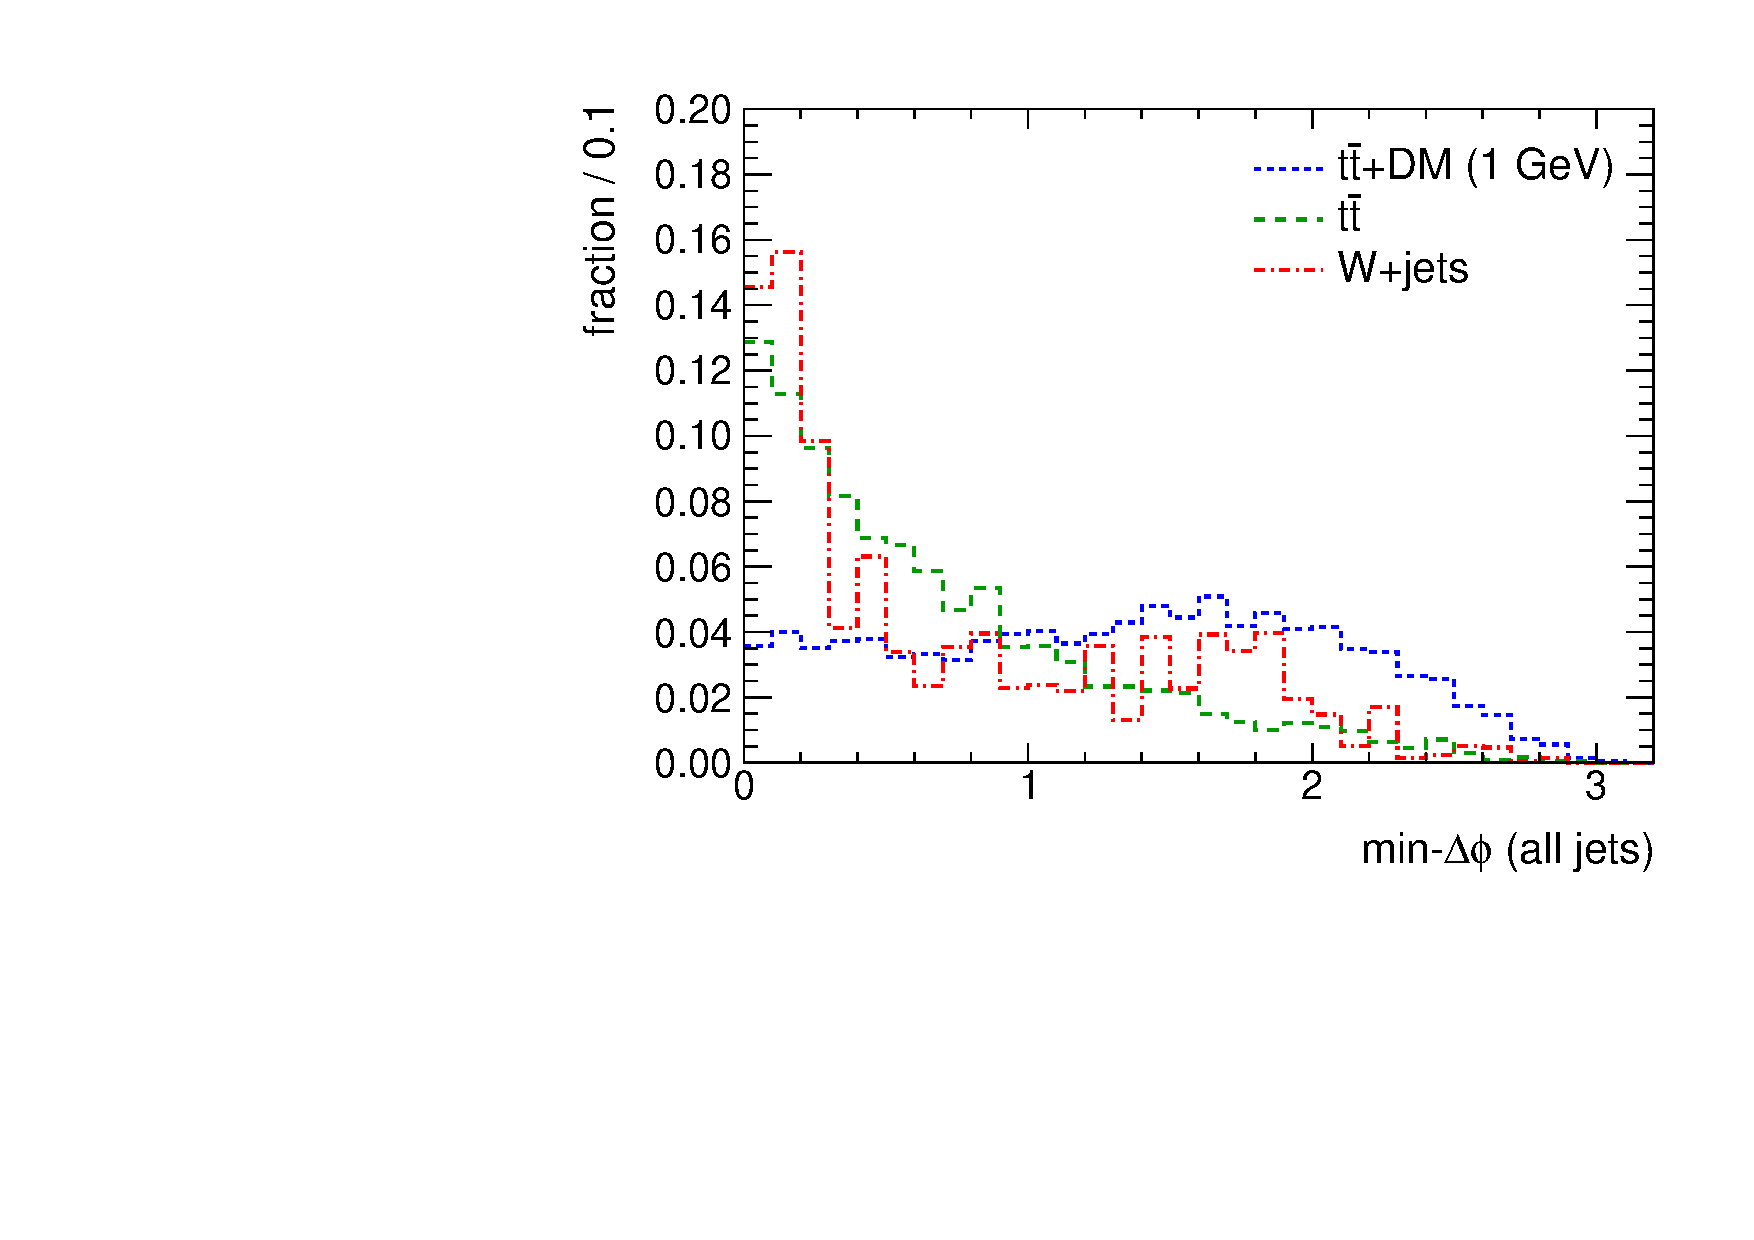
\includegraphics[width=0.32\textwidth]{figures/semilept-overlay-dphijetmet.pdf}
  \caption{$\Delta\phi$ distributions for $\Wjets$, $\ttbar$, and $\ttbar+$DM signal ($M_\chi = 1\:\GeV$). Histograms are normalized to unit area.}
  \label{fig:semilept_overlay_dphijetmet}
\end{figure}

The performance of the different $\Delta\phi$ definitions are summarized in background versus signal efficiency curves for $\Wjets$ and $\ttbar$ shown in Fig.~\ref{fig:semilept_dphijetmet_roc}. The definitions with two and with three jets perform best, depending on the desired signal efficiency or background efficiency. Input from data and more realistic MC, as well as a better understanding of systematic uncertainties, will determine the best definition and working point.

\begin{figure}[htbp]
  \centering
  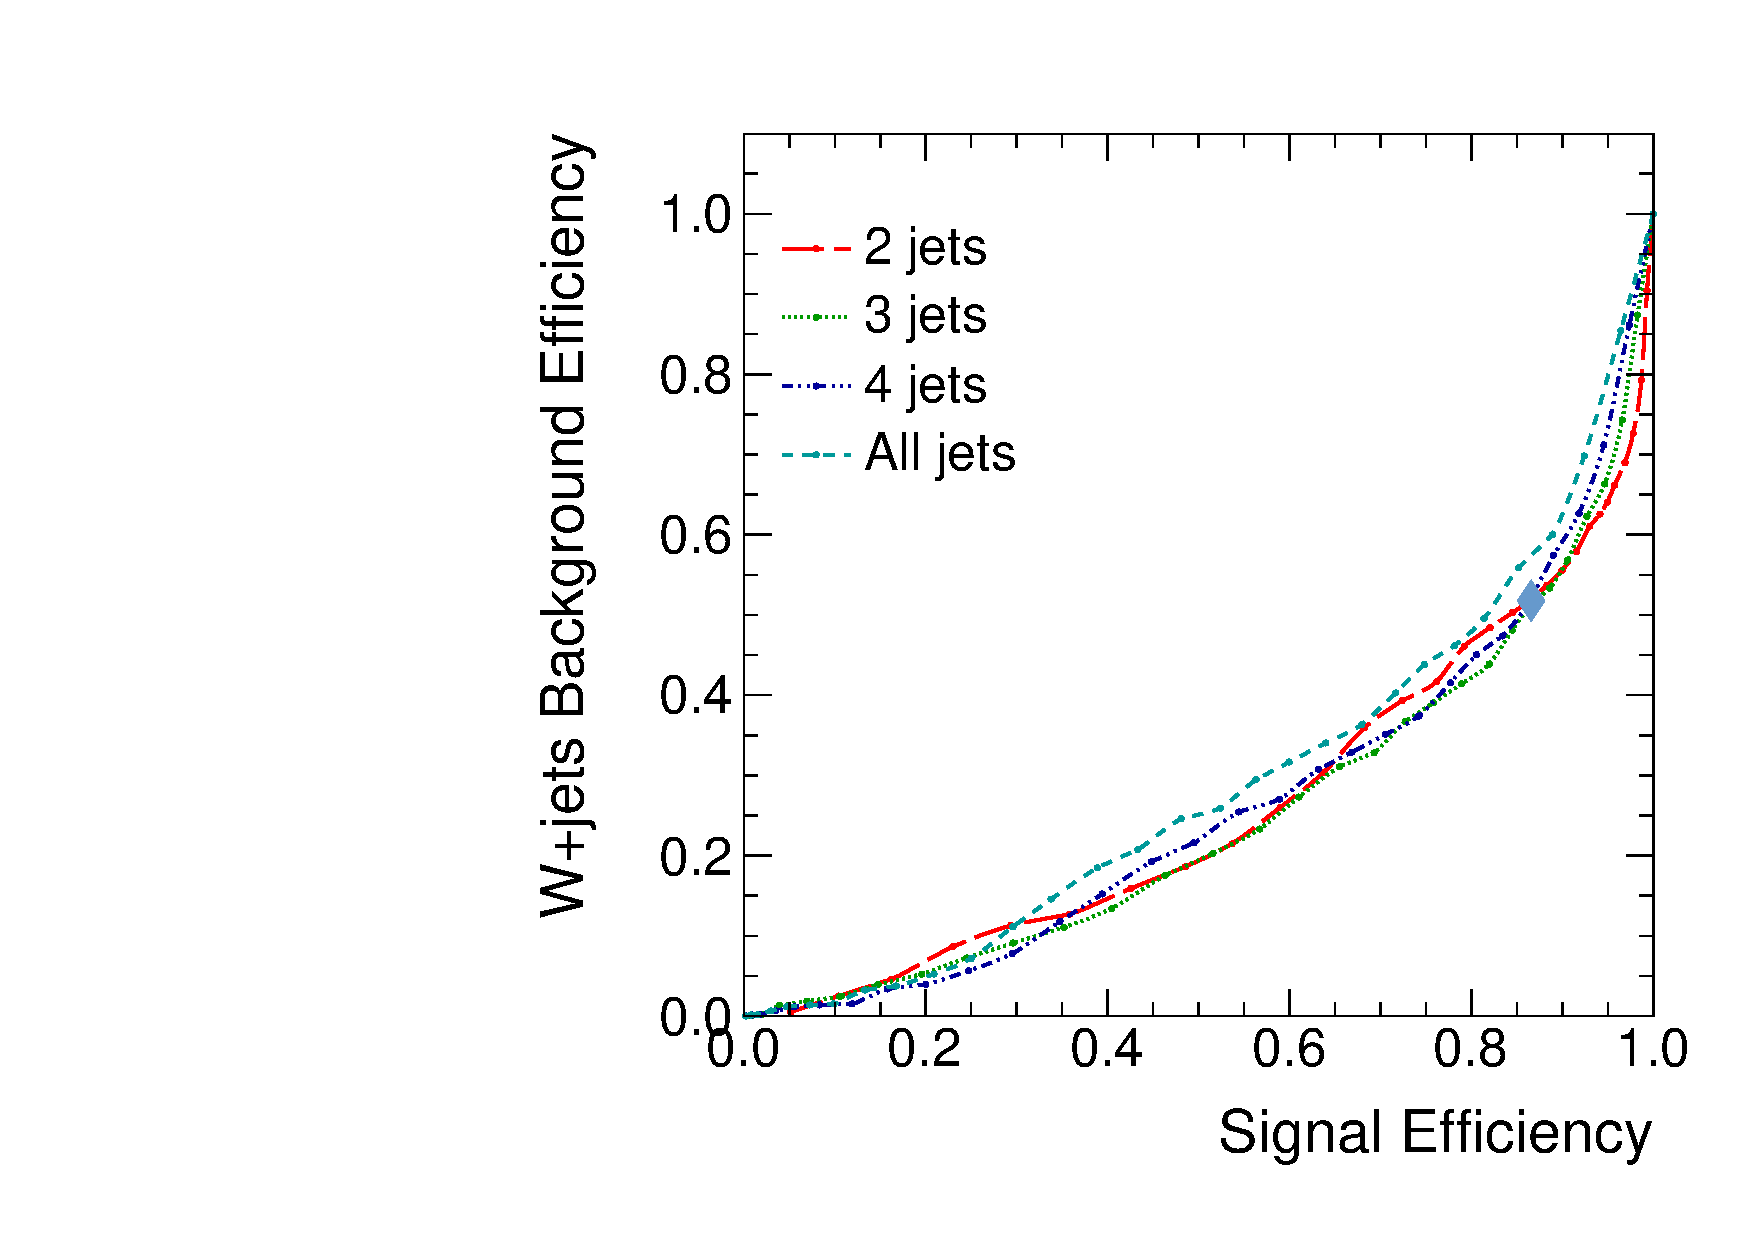
\includegraphics[width=0.32\textwidth]{figures/ttdm1_vs_wjets-semilept-roc.pdf}
  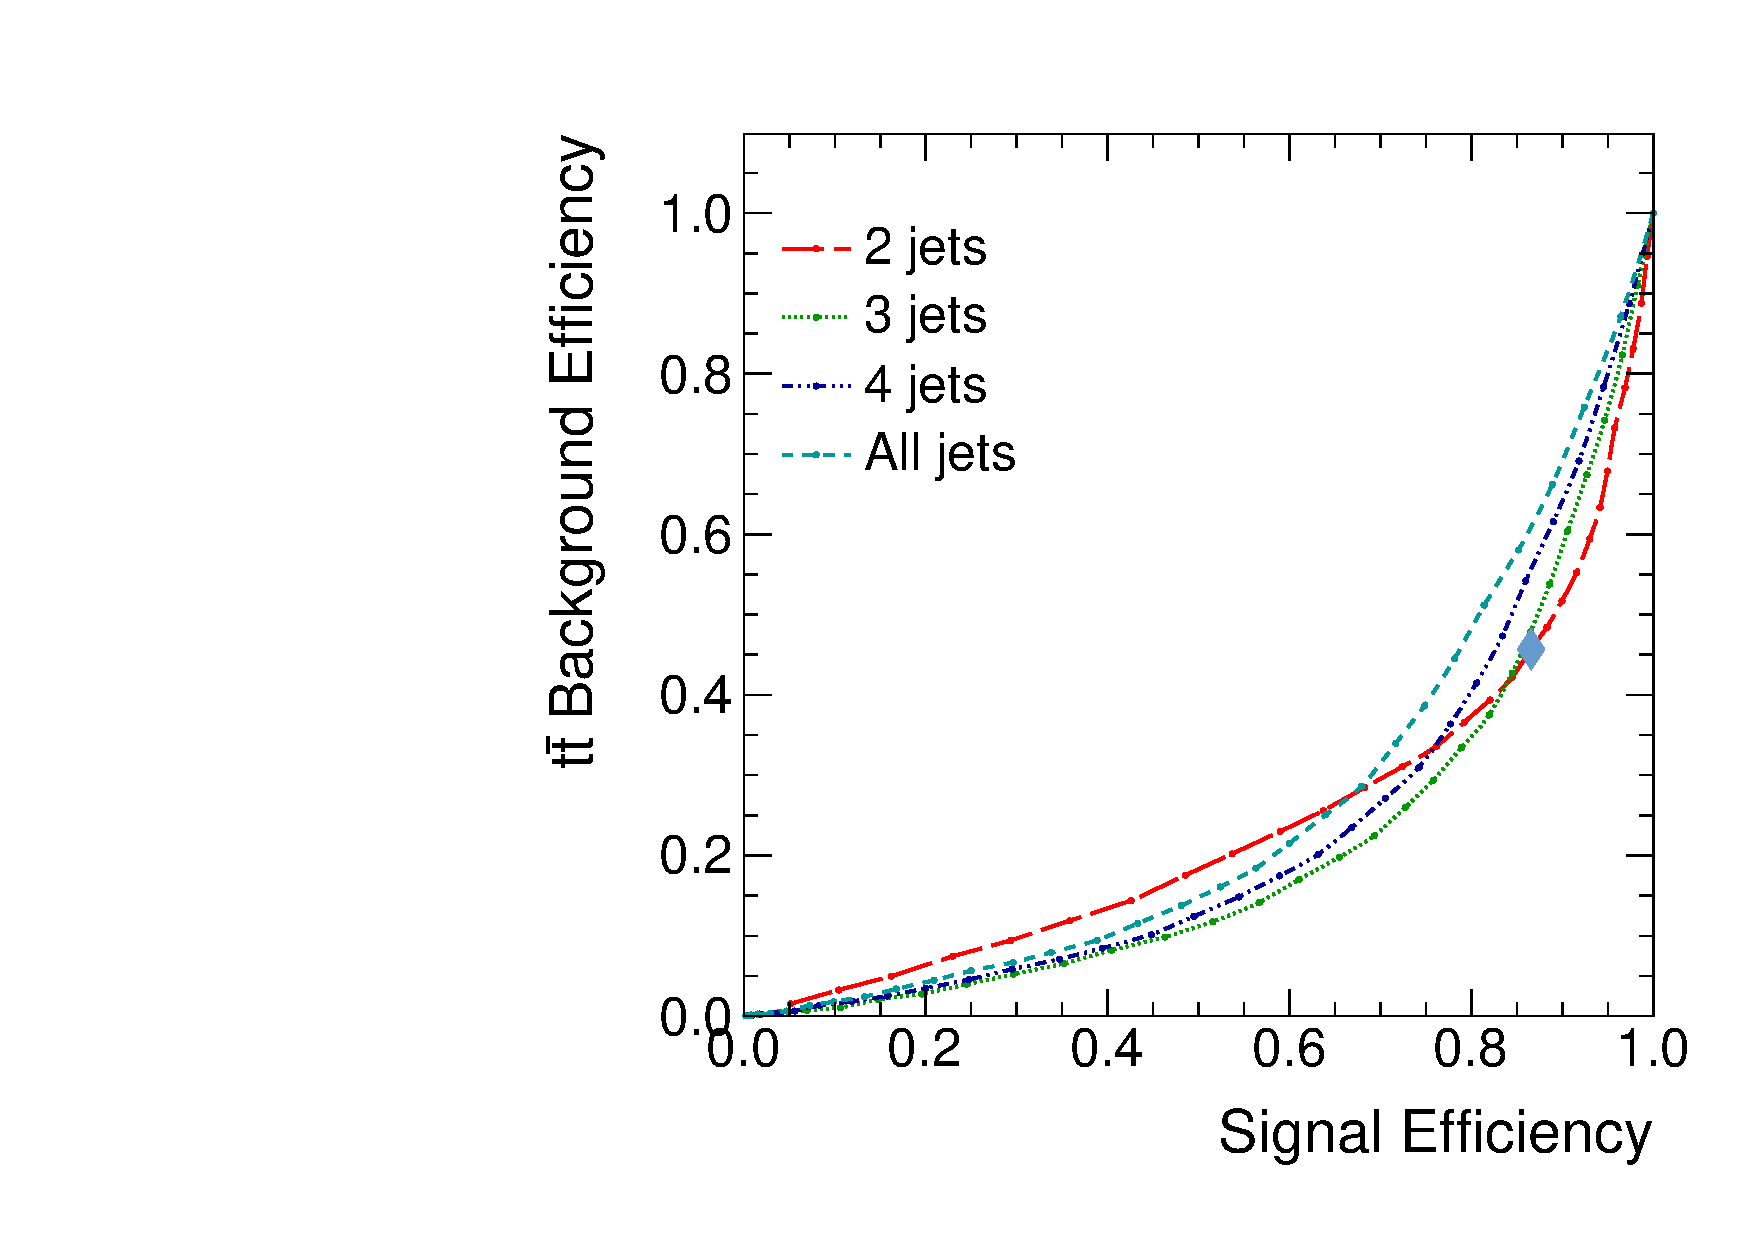
\includegraphics[width=0.32\textwidth]{figures/ttdm1_vs_ttbar-semilept-roc.pdf}
  \caption{Background versus signal efficiency curves for various $\Delta\phi$ definitions. The diamond marker indicates the operating point corresponding to the $\min_{i=1,2}\Delta\phi\left(j_i,\met\right)$ cut used in the inclusive semileptonic selection.}
  \label{fig:semilept_dphijetmet_roc}
\end{figure}
